% gjilguid2e.tex
% V2.0 released 1998 December 18
% V2.1 released 2003 October 7 -- Gregor Hutton, 
% updated the web address for the style files.

\documentclass[extra]{gji}
\usepackage{graphicx}
\usepackage{subcaption}
\usepackage{timet}
\usepackage[fleqn]{amsmath}
\usepackage{mathrsfs}
\usepackage{amssymb}
\usepackage{mathtools} 
\usepackage{bbm}
\usepackage[Symbol]{upgreek}
\usepackage{hyperref}
\hypersetup{
     colorlinks = true,
     citecolor  = blue,
     linkcolor  = blue,
     urlcolor   = blue 
}
\captionsetup{compatibility=false}
\setlength{\parindent}{9pt}
\allowdisplaybreaks
\captionsetup[subfigure]{labelformat=simple}
\renewcommand\thesubfigure{(\alph{subfigure})}

\title[Waves in 3-D Earth]
  {Efficient global wave propagation adapted to 3-D structural complexity: 
  a pseudo-spectral/spectral-element approach}
\author[K Leng et al.]
  {Kuangdai Leng$^{1, 2}$, Tarje Nissen-Meyer$^1$ and Martin van Driel$^3$\\
  $^1$ Department of Earth Sciences, University of Oxford, South Parks Road,
  Oxford \emph{OX1 3AN}, United Kingdom\\
  $^2$ Key Laboratory of Transportation Tunnel Engineering, Southwest Jiaotong University, 
  Chengdu \emph{610031}, China\\
  $^3$ Institute of Geophysics, ETH Zurich, 
  Sonneggstrasse \emph{5, 8092} Zurich, Switzerland}
\date{Received 1998 December 18; in original form 1998 November 22}
\pagerange{\pageref{firstpage}--\pageref{lastpage}}
\volume{200}
\pubyear{1998}

\let\leqslant=\leq
\newtheorem{theorem}{Theorem}[section]
\begin{document}
\label{firstpage}
\maketitle


\begin{summary}
  We present a new, computationally efficient numerical method to
  simulate global seismic wave propagation in realistic 3-D Earth models.
%   
  We characterize the azimuthal dependence of 3-D wavefields in 
  terms of Fourier series, such that the 3-D equations of motion reduce to 
  an algebraic system of coupled 2-D meridian equations, 
  which is then solved by a 2-D spectral element method (SEM).
%   
  Computational efficiency of such a hybrid method stems from 
  lateral smoothness of 3-D Earth models and axial singularity of seismic point sources, 
  which jointly confine the Fourier modes of wavefields to a few lower orders. 
%  
  We show novel benchmarks for global wave solutions in 3-D structures 
  between our method and an independent, fully discretized 3-D SEM
  with remarkable agreement.
%  
  Performance comparisons are carried out on three state-of-the-art tomography 
  models, with seismic period ranging from 34s down to 11s.
%   
  It turns out that our method has run up to two orders of magnitude faster than the 
  3-D SEM, featured by a computational advantage expanding with seismic frequency. 
\end{summary}

\begin{keywords}
  numerical solutions; computational seismology; theoretical seismology; 
  wave propagation
\end{keywords}

%%%%%%%%%%%%%%%%%%%%%%%%%%%%%%%%%%%%%%%%%%%%%%%%%%%%%%%%%%%%%%%%%%%%%%%%%%%%%%%%
\section{Introduction}
Earth structure and dynamics are largely inferred by seismology 
as the main tool for data-informed probing of Earth's interior. 
Starting from a spherically layered view, e.g., 
the PREM model \cite[]{dziewonski1981prem}, 
the last few decades have revealed consensual pictures of a 3-D
interior featured by large-scale thermal and compositional heterogeneities 
\cite[]{becker2002comparison}.
To obtain such images, one needs to compare measurements from observed and synthetic seismograms. 
As such, simulations of global seismic wave propagation in physically realistic 
Earth models have been attracting increasing interest. 
Such simulations capture the physics of seismic wavefields  
most accurately and are emerging as effective tools for 
modern seismic tomography \cite[]{tromp2005seismic, 
nolet2008breviary, rawlinson2010seismic}.

Despite a surge in both hardware and software developments,
global wavefield simulations remain computationally challenging, 
especially for tomographic inverse problems and when targeted at high frequency resolutions 
(e.g. seismic period \textless 10s) where a wealth of open geophysical 
questions harbor. The bottleneck of computing power is foiled
by an exponentially increasing number of observed broadband data
(IRIS annual report 2015, \url{iris.edu}), from which abundant
information is still excluded, such as a number of source-receiver pairs,
amplitude information, and/or high-frequency contents.
To probe deeper into the problem, let us first look at 
forward waveform modeling and then seismic tomography.

\subsection{Forward modeling}
To analyze and understand observed seismograms in terms of their source
characteristics or structure-induced propagation effects, one needs to
solve the forward problem of seismic wave propagation.

In recent decades, full 3-D numerical methods have become increasingly
commonplace, e.g.,
finite difference \cite[]{igel2002wave}, 
discontinuous Galerkin \cite[]{dumbser2006arbitrary},
and spectral element methods \cite[]{komatitsch2002spectralI, 
komatitsch2002spectralII, chaljub2007spectral, peter2011forward}.
These comprehensive methods tackle complex 3-D structures in
various geometries, and are thus to be considered ``full'' and
``exact'' so long as numerical discretization errors are kept small. 
Unfortunately, such full 3-D methods come at a persistently high 
computational cost that still obliterates any possibility to 
cover the entire recorded frequency band (e.g. 1Hz) in the
foreseeable future for actual applications, 
especially for tomographic inverse problems that involve 
thousands to millions of simulations.

Efforts to decrease computational cost have relied on hardware 
accelerators such as GPU \cite[]{komatitsch2011fluid, rietmann2012forward},
algorithmic advances such as improved time schemes 
\cite[]{rietmann2015load, ma2014low, nissen2008sem}, 
cache-optimized tensor products \cite[Chap 8,][]{deville2002high,
nissen2007sem}, and coarse-grained attenuation \cite[]{van2014optimized}.
Most of these efforts lead to a computational speedup
of 2 to 5. This is most desirable, especially in its multiplicative effect,
but does not bear ``game-changing'' qualities.

Computability can furthermore be eased by well-chosen approximations 
on the physical system. 
Global seismic data analysis, for instance, largely clusters around seismic traveltimes 
or waveforms predicted by spherically symmetric Earth models \cite[]{rawlinson2010seismic,
driel2015instaseis}.
Under this simplification, methodological and computational advances have remarkably progressed 
from ray-theoretical solutions \cite[]{jeffreys1958seismological} 
to normal-mode summation \cite[e.g., Chap 8,][]{dahlen1998theoretical},
fast full-waveform methods such as
DSM \cite[]{kawai2006complete}, GEMINI \cite[]{friederich1995complete} and 
Yspec \cite[]{al2008calculation}, 
and fast full-wavefield methods such as AxiSEM \cite[]{nissen2014axisem}, an axisymmetric SEM, and 
axisymmetric finite difference methods \cite[]{igel1995sh, toyokuni2006fdm}. 
If small deviations in the recorded waveforms from such a structural setting
are tolerable, one may revert to computing 3-D global wavefields based on
1-D averaged models \cite[e.g. PREM,][]{dziewonski1981prem}, 
which can be accomplished at the cost of a 2-D
numerical method by exploiting axisymmetry in the wave solution
\cite[]{nissen2007axisem}. 
With increasing frequency, axisymmetric methods become 
several orders of magnitude faster than full 3-D methods \cite[]{nissen2014axisem}. 
This has been viable as a basis for global tomography 
\cite[]{rawlinson2010seismic}, allowing for full-wave based calculation 
of sensitivity kernels \cite[]{colombi2012kernels} and data-matched 
high frequency resolutions \cite[e.g. 1Hz,][]{hosseini2015multifrequency}. 
Spherically symmetric Earth models, as summarized by \cite{nissen2014axisem},
can thus be viewed as a pragmatic compromise for modeling between broad
frequency ranges and reasonably realistic waveforms, so as to exploit 
a maximal amount of informative broadband data.
Other physical approximations may operate on rheology 
\cite[e.g., acoustic approximation, ][]{zhu2009elastic}
or structural complexity by means of homogenization \cite[]{capdeville2013residual}.

The computational cost of fully discretized 3-D methods is model-agnostic. 
It is then implied by the tremendous speedup of axisymmetric methods 
(e.g. AxiSEM) that those 3-D methods may lavish a large 
amount of computing power on model oversampling, not only for radial models but 
also for 3-D models with smooth, long-wavelength lateral structures.  
In this paper, we shall be concerned with bridging the gap between 
fast methods for spherically symmetric media and slow methods for
complex 3-D media by means of developing a method fully 
adapted to model complexity. 
The method is expected to be most efficient for 
Earth models that are laterally smooth relative to seismic wavelengths, 
but is to be seen as a fully convergent, general numerical wave solver. 
In this context, we shall
now examine the nature of existent tomographic models as well as their
underlying, continually developing methodologies.

\subsection{Seismic tomography}
\label{sec:tomography}
Most global tomographic models exhibit excellent agreement on the 
predominant long-wavelength features in the mantle,
see reviews of \cite{becker2002comparison} and \cite{auer2014savani}. 
For smaller-scale structures, however, those models tend to disagree to a 
greater extent, and such divergence has persisted to the present day
despite advances in data coverage and inverse techniques. 
Though we seem to face a significant challenge in finding consensus, which 
may or may not hint at a deeper issue than refined coverage or techniques,
acquisition (e.g. transportable arrays) and measurement developments 
in conjunction with more sophisticated tomographic methods
inevitably lead to more profound understanding of observations
and more reliable inference of Earth's interior.

From a measurement perspective, 
seismic tomography has been experiencing transformative progress
from ray theory \cite[]{rawlinson2010seismic} to waveform based
inversions \cite[]{tape2009adjoint, fichtner2008theoretical}. 
This is partly because, on one hand,
most modern measurements of ``traveltimes'', 
such as cross-correlation \cite[Chap 7,][]{nolet2008breviary}, 
time-frequency phase delays \cite[]{fichtner2008theoretical, 
kristekova2009time} and instantaneous phase \cite[]{bozdaug2011misfit}, 
are based upon waveforms,
and on the other hand, triplicated \cite[]{stahler2012triplicated} or 
core-diffracted phases \cite[]{bharadwaj2013enhancing, hosseini2015multifrequency} 
and noise correlations \cite[]{basini2013influence} inherently 
necessitate waveforms as well.
Therefore, fast waveform modeling across a broad frequency band
becomes increasingly important as seismologists attempt to extract  
more information from complex seismic data. 

Computational challenges stem not only from complexity in data space 
but also from that in model space, limiting the application 
of the next-generation tomographic methods.
An essential step in seismic tomography is to calculate  
Fr\'{e}chet sensitivity kernels
for particular misfit functionals, see e.g., \cite{dahlen2000frechet}
for finite-frequency traveltimes and Chap 4, \cite{nolet2008breviary}
for full wavefields. 
A fundamental principle behind the ``kernels'' is that 
structural perturbations from background models
should be sufficiently small such that the first-order
Born approximation, or a linearized relation between the perturbations of 
response and structure, can decently hold. 
Thus, starting from 3-D background models characterized by well-accepted 
long-period structures should be a reasonable and promising choice.
The last decade has witnessed the tendency toward  
tomography with kernels based on 3-D background models and waveform-based misfit
functionals, from exploration 
\cite[e.g.,][]{plessix2006review, luo2009seismic}
to continental/global scale
\cite[e.g.,][]{liu2008finite, tape2009adjoint, fichtner2008theoretical, colombi2014seismic}, 
mainly using adjoint approaches \cite[]{tarantola1988theoretical,
tromp2005seismic} built upon high performance 
SEM \cite[]{komatitsch2002spectralI, peter2011forward}.
Thanks to the self-adjointness of elastodynamics, the underlying wave solvers are
identical to those used for forward simulations, i.e., the kernels are 
constructed by convolving a wavefield emanating from a seismic source with a
receiver-originating adjoint wavefield that bears the misfit functional.
Unfortunately, the formidable cost of global wave simulations
(that need to be repeated numerous times for each waveform inversion) 
keeps high-resolution adjoint tomography far from being 
available as common practice, especially in view of data availability.

Our initial consensus on the predominance of long-wavelength 
heterogeneity in the mantle \cite[]{su1991predominance} suggests that
it is impractical (if not unwise from an inversion convergence
perspective) to introduce localized small-scale 3-D structures
into background models. 
Horizontal interfaces or sharp gradients may of course exist in the deep interior, 
yet none of our available tomographic models show evidence as can be 
deduced from the finite power spectra \cite[]{becker2002comparison},
inasmuch as tomography delivers models with heterogeneities much larger than the
wavelengths by construction.
After all, neither data coverage nor the mostly linearized inversion 
methodology can account for such strong lateral variations.
In short, the vast majority of simulations for tomographic purposes are
performed upon considerably smooth models with respect to seismic 
wavelengths. Therefore, based on its model-adaptive cost characteristic, 
our method should be more suitable than full 3-D methods 
as the underlying wave solver.   

% In addition, the model adaptivity also maximizes the
% flexibility to construct ``hypothetical'' but most relevant 3-D background models,
% further facilitating tomography by exploiting other favorable structural and 
% geometric features, as will be elaborated later.  

This paper is organized as follows. The following methodological section
provides a brief but essentially integrated overview of the method, 
including wavefield and model observations, physical motivations and 
method architecture. 
In Section~\ref{sec:theory}, we present the full theory that rebuilds the 
3-D equations of motion on a 2-D meridian domain, with emphasis placed on 
axial singularity of seismic point sources and a narrowly banded 
structure of the dimension-reduced algebraic system. Section~\ref{sec:imp} 
briefly introduces our SEM implementation of the theory, as a
generalization of the axisymmetric method AxiSEM \cite[]{nissen2014axisem}. 
In Section~\ref{sec:ben}, we benchmark the method in reference to
an independent 3-D SEM, SPECFEM3D\_GLOBE 
\cite[SPECFEM,][]{komatitsch2002spectralI, 
komatitsch2002spectralII}, considering frequency and source influences. 
It is then followed by the performance section where we compare the
efficiency of the two methods using three state-of-the-art tomographic models.
The last section summarizes the main results and features, and 
ends up with an outlook for future developments.  

%%%%%%%%%%%%%%%%%%%%%%%%%%%%%%%%%%%%%%%%%%%%%%%%%%%%%%%%%%%%%%%%%%%%%%%%%%%%%%%%
\section{Methodology}
We seek to compute the 3-D global seismic wavefield produced by a realistic 
earthquake source in an anisotropic visco-elastic 3-D Earth model. 
One may treat the problem as general as seismic wave propagation 
in a 3-D heterogeneous medium and solve it with a ``universal'' 3-D 
numerical method such as SPECFEM. 
But one may also take a shortcut by understanding the particularities 
first and using them to simplify the general wave equation at the outset, 
e.g., \cite{nissen2007axisem} for spherical symmetric Earth models.
Following this idea, we shall start from direct observations of 
wavefield snapshots in tomographic models, which may inspire some
facilitative spatial characteristics. 

%~~~~~~~~~~~~~~~~~~~~~~~~~~~~~~~~~~~~~~~~~~~~~~~~~~~~~
\subsection{Seismic wavefields in 3-D global structures}
\label{sec:snap}
For visualization purposes, we employ an earthquake source 
of monopole type, i.e.,
$M_{rr}=1$ and the other components of the moment tensor vanish,
located at a 12km's depth beneath Virginia. 
Such a source is fully axisymmetric in the source-centered coordinate system 
shown in Fig.~\ref{fig:sk}.
See \cite{nissen2007axisem} or Section~\ref{sec:moment} for a strict 
definition of monopole sources. 
To be objective, we use SPECFEM to compute the wavefields. 

Let us first consider 1-D models. Evidently, the displacement response 
should be fully axisymmetric due to the axisymmetry of both the source 
and the model, as illustrated by Fig.~\ref{fig:1deq} using PREM as a 
background model \cite[]{dziewonski1981prem}.
By contrast, the wavefield exhibits high complexity in the meridional 
slice plane orthogonal to the azimuthal direction, as shown in Fig.~\ref{fig:1dsl}. 
The reason behind this contrast will be given in Section~\ref{sec:moment}.
Since the solution is rotation invariant, i.e., 
$u\left(r,\theta,\phi; t\right)=u\left(r,\theta; t\right)$, 
the 3-D problem can be rebuilt on a 2-D meridian domain (slice plane)
spanned by $\left(r,\theta\right)$, 
and solved efficiently \cite[]{nissen2014axisem}. 

For 3-D models, the solution axisymmetry is violated by lateral 
heterogeneity, as illustrated by Fig.~\ref{fig:3deq}
using the tomographic model s40rts 
\cite[]{ritsema2011s40rts}. But, even by visual inspection, 
one may observe that the non-axisymmetric deviations are quite ``small'', 
i.e., the equatorial pattern (Fig.~\ref{fig:3deq}) looks much smoother 
than the slice pattern (Fig.~\ref{fig:3dsl}). 
Hence, from a numerical aspect, it is unnecessary to describe the azimuthal 
variations using grid points distributed as densely as required to 
describe the in-slice variations. Let us instead parameterize 
the azimuthal dependence by Fourier series, considering the azimuthal
periodicity of solution over $[0,2\pi)$, 
\begin{equation}  
  u\left(r,\theta,\phi;t\right) \simeq \sum_{|\alpha| \le N_u} 
  u^\alpha\left(r,\theta;t\right)\exp\left(\mathbbm{i}\alpha\phi\right),
  \label{eq:demo}
\end{equation}
where $N_u$ denotes the global maximum number of terms needed for an accurate 
description, $u^\alpha$ the $\alpha$-th order complex Fourier coefficient 
field\footnote{In this paper, superscripts acting \textit{directly} on 
field variables denote Fourier series indices; e.g., $\rho^2$ represents the 
second order Fourier coefficient of $\rho$, whereas the square of $\rho$, if
needed, is written as $\left(\rho\right)^2$.}, 
$t$ the time and $\mathbbm{i}=\sqrt{-1}$. 

The separation of variables in \eqref{eq:demo} is 
adapted to the dimension-dependent variability of global wavefields, that is, 
a small $N_u$ may realize an accurate description of smooth azimuthal variations, 
while the 2-D coefficient fields, $u^\alpha=u^\alpha\left(r,\theta;t\right)$, 
are capable of describing any sharp in-slice variations. 
Such an idea may date back to 1980's in a series of studies by 
\cite{alekseev1980solution, mikhailenko1984synthetic,
mikhailenko1984calculation} for layered media at a local scale, but
was never implemented for real 3-D media. 
For instance, Fig.~\ref{fig:four} shows the Fourier approximations at
the equatorial great circle, where the wavefield in Fig.~\ref{fig:3deq} 
experiences the largest azimuthal variability during the snapshot moment. 
It is shown that a Fourier series with $N_u=40$ visually yields
an exact description, while full 3-D discretization along the great circle
in SPECFEM involves 4096 (256$\times$4$\times$4) Gauss-Lobatto-Legendre (GLL) 
points at the considered dominant period 17s. 

Fourier characterizations such as \eqref{eq:demo} involves global expansion of 
functions over the $\phi$-dimension, and thus fall into the category of 
pseudo-spectral methods, which can be equivalently interpreted by means of 
cardinal functions \cite[Chap 5,][]{boyd2001spectral}.
For instance, the cardinal version of Equation~\eqref{eq:demo} reads
\begin{equation}
  u\left(r,\theta,\phi;t\right)=\sum_{\beta=0}^{2N_u} 
  u\left(r,\theta,\phi_\beta;t\right)C_\beta\left(\phi\right),\quad 
  \phi_\beta=\frac{2\pi \beta}{2N_u+1},
  \label{eq:card}
\end{equation}
where $C_\beta\left(\phi\right)$ are shifted sinc functions (cardinal functions
associated with Fourier series) such that 
$C_\beta\left(\phi_\gamma\right)=\delta_{\beta\gamma}$.   
Points at the same $\phi_\beta$ assemble what we call slices. 
We do not use cardinal functions directly in this paper. 
But, since they bridge the two field representation methods respectively  
by means of basis functions and grid points, 
they may facilitate the understanding of fundamental concepts 
(e.g., mode coupling in Section~\ref{sec:strong}) and comparisons
to fully discretized 3-D methods. For instance, a good approximation
of Fig.~\ref{fig:3deq} requires 41 complex terms in the 
Fourier series, or, interpreted as cardinal functions, 
81 slices evenly spaced by $\sim$4.4\degr around the axis, 
which are much fewer than the grid points required by the 
3-D discretization.     

\begin{figure*}
  \centering
  \begin{minipage}{0.4\textwidth}
    \centering
    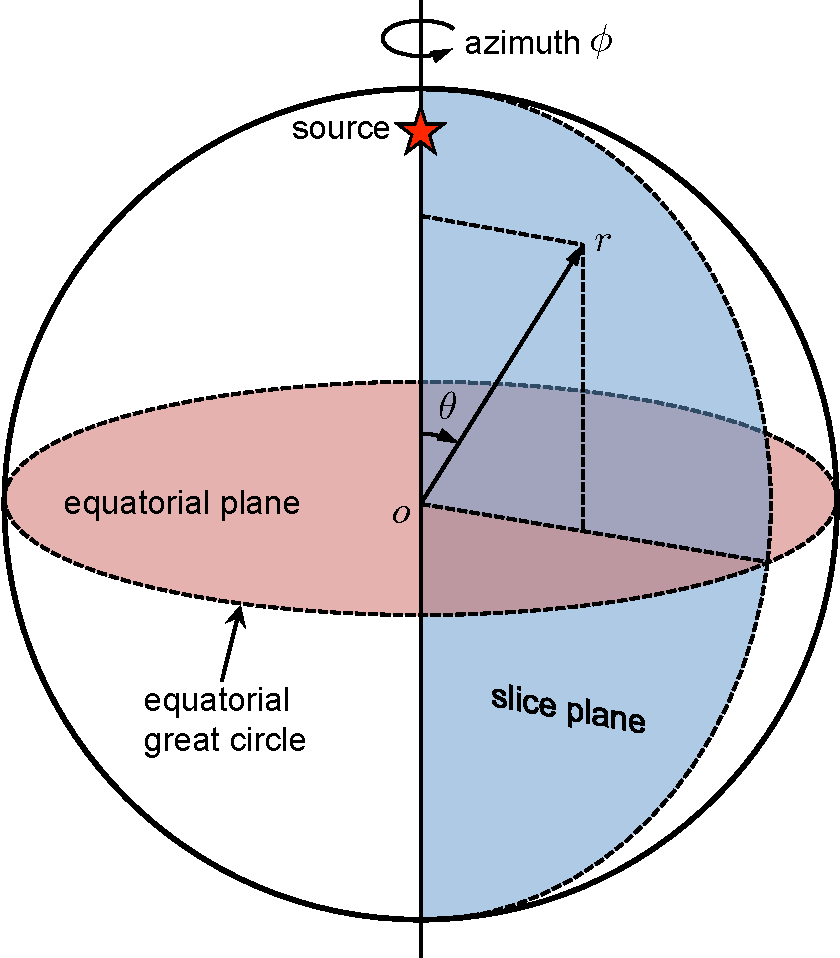
\includegraphics[width=.9\textwidth]{fig/snapshot/sketch.pdf} 
    \subcaption{sketch}
    \label{fig:sk}
  \end{minipage}%
  \begin{minipage}{0.6\textwidth}
    \begin{minipage}{.585\textwidth}
      \centering
      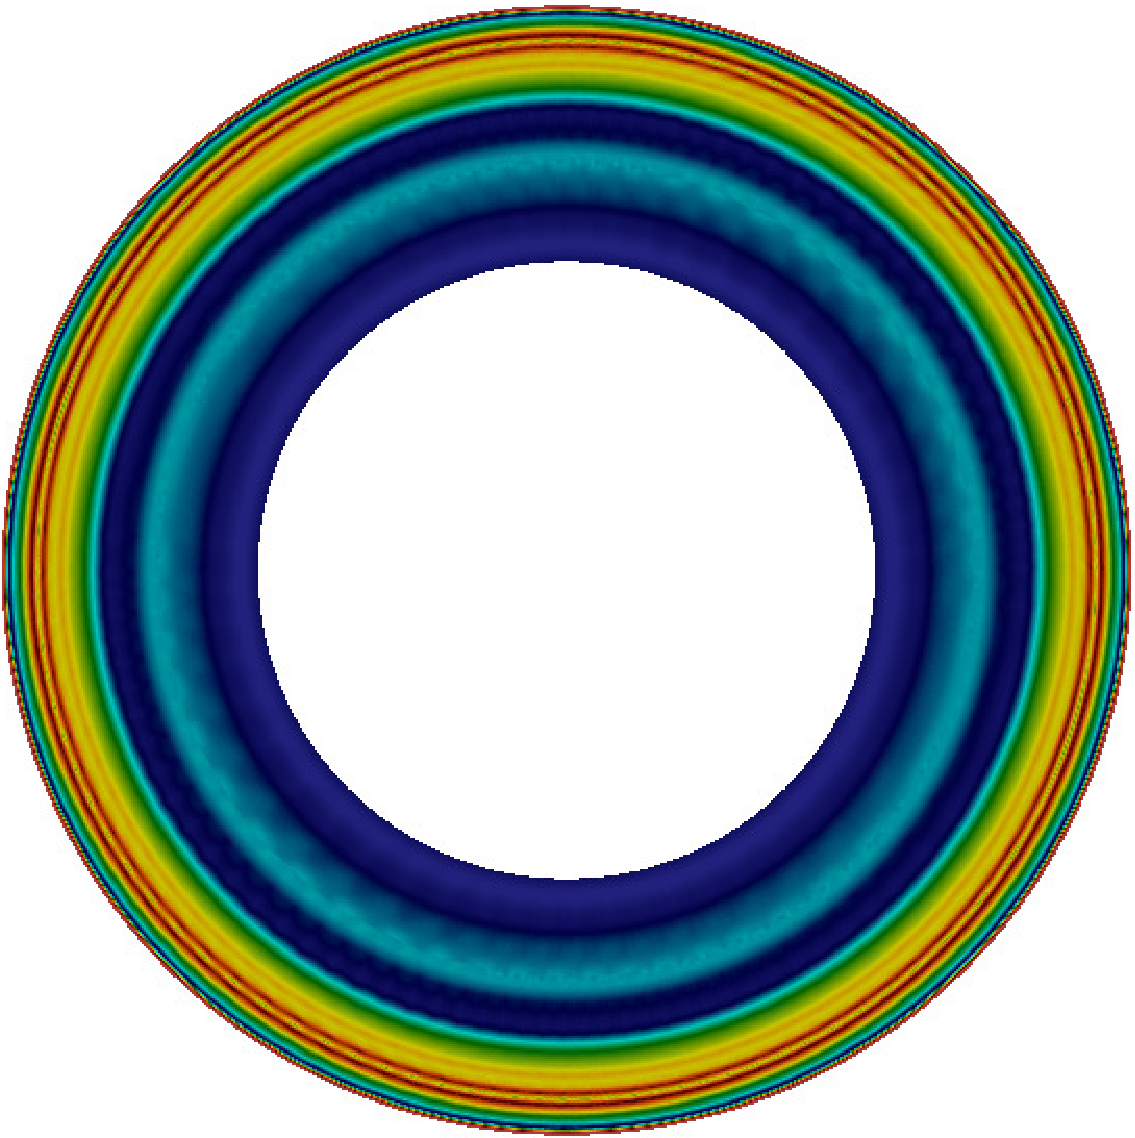
\includegraphics[height=.85\textwidth]{fig/snapshot/1d-phi.pdf}
      \subcaption{1-D equatorial}
      \label{fig:1deq}  
    \end{minipage}
    \begin{minipage}{.39\textwidth}
      \centering
      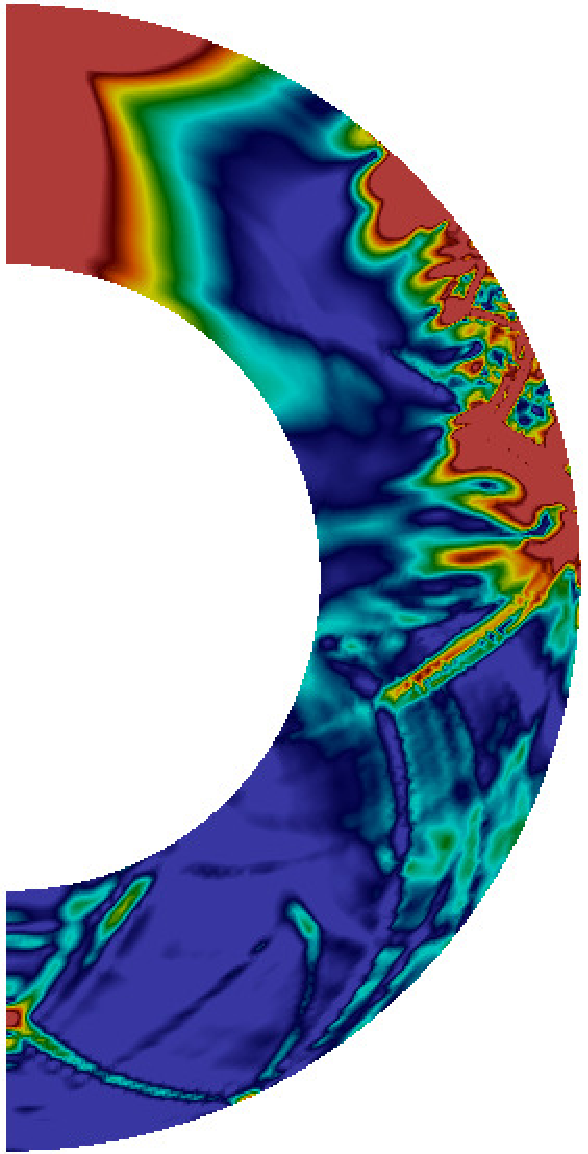
\includegraphics[height=1.275\textwidth]{fig/snapshot/1d-slice.pdf}
      \subcaption{1-D slice}
      \label{fig:1dsl}    
    \end{minipage}\\
    \begin{minipage}{.585\textwidth}
      \centering
      \vspace{1em}
      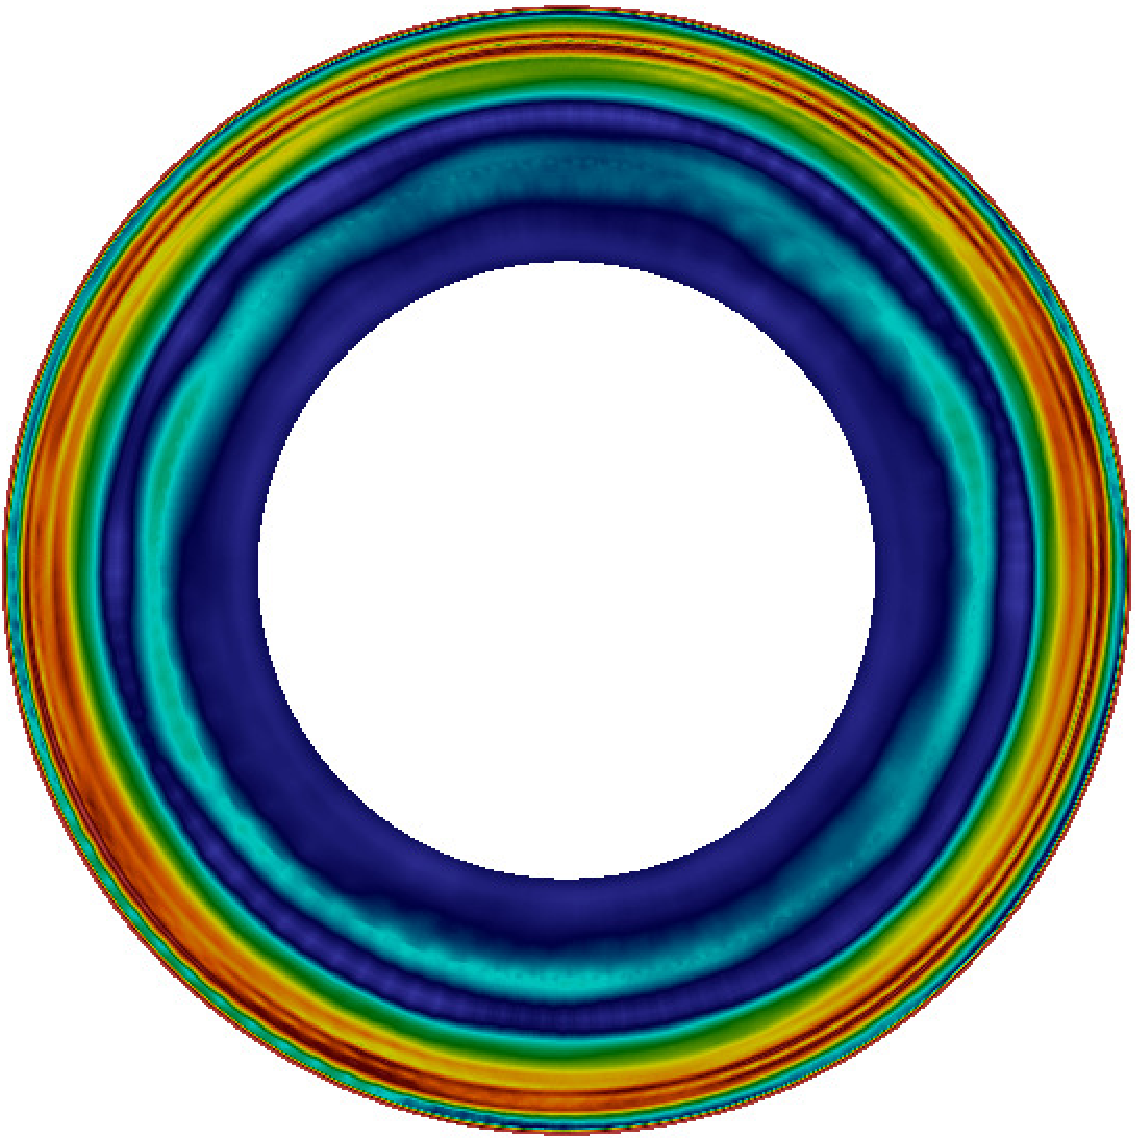
\includegraphics[height=.85\textwidth]{fig/snapshot/3d-phi.pdf}
      \subcaption{3-D equatorial}
      \label{fig:3deq}  
    \end{minipage}
    \begin{minipage}{.39\textwidth}
      \centering
      \vspace{1em}
      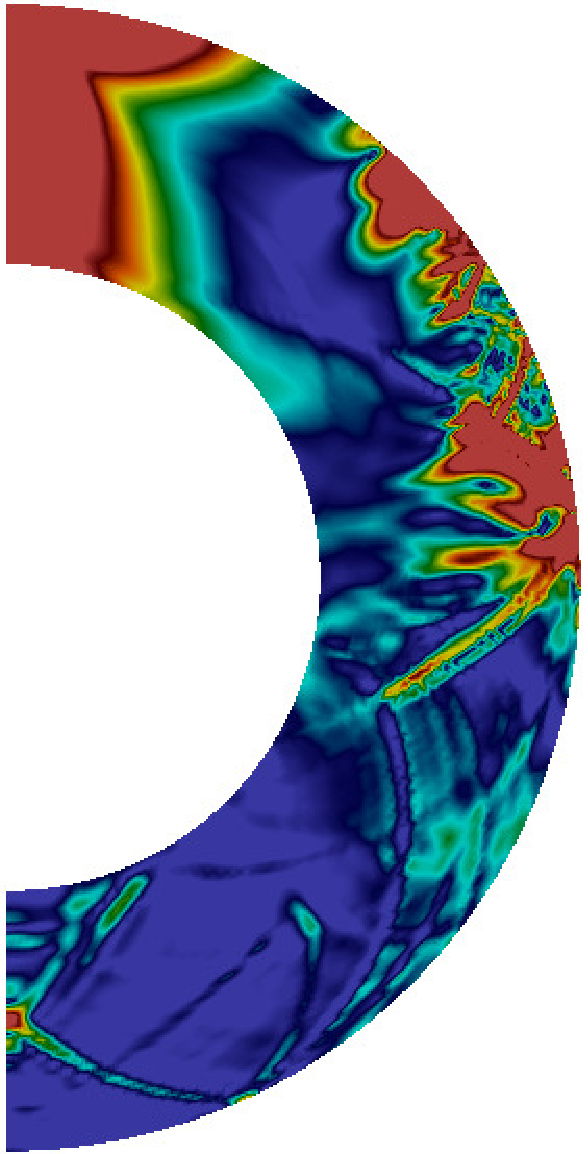
\includegraphics[height=1.275\textwidth]{fig/snapshot/3d-slice.pdf}
      \subcaption{3-D slice}
      \label{fig:3dsl}    
    \end{minipage}
  \end{minipage}%
  \caption{Wavefield snapshots in 1-D model 
  PREM and 3-D model s40rts due to a monopole source, 
  computed by SPECFEM at a dominant period of 17s. 
  The snapshots are taken at $\sim$1430s after source origin 
  and the color function shows displacement norm. 
  The core regions are not plotted because displacement calculation
  in the fluid core is not implemented in SPECFEM. 
  (a) shows a sketch of source-centered coordinate system and 
  positions of the equatorial and slice planes. 
  (b)-(e) show the snapshots on the two planes across the two models, respectively.}
  \label{fig:snapshot}
\end{figure*}

\begin{figure*}
  \centering
  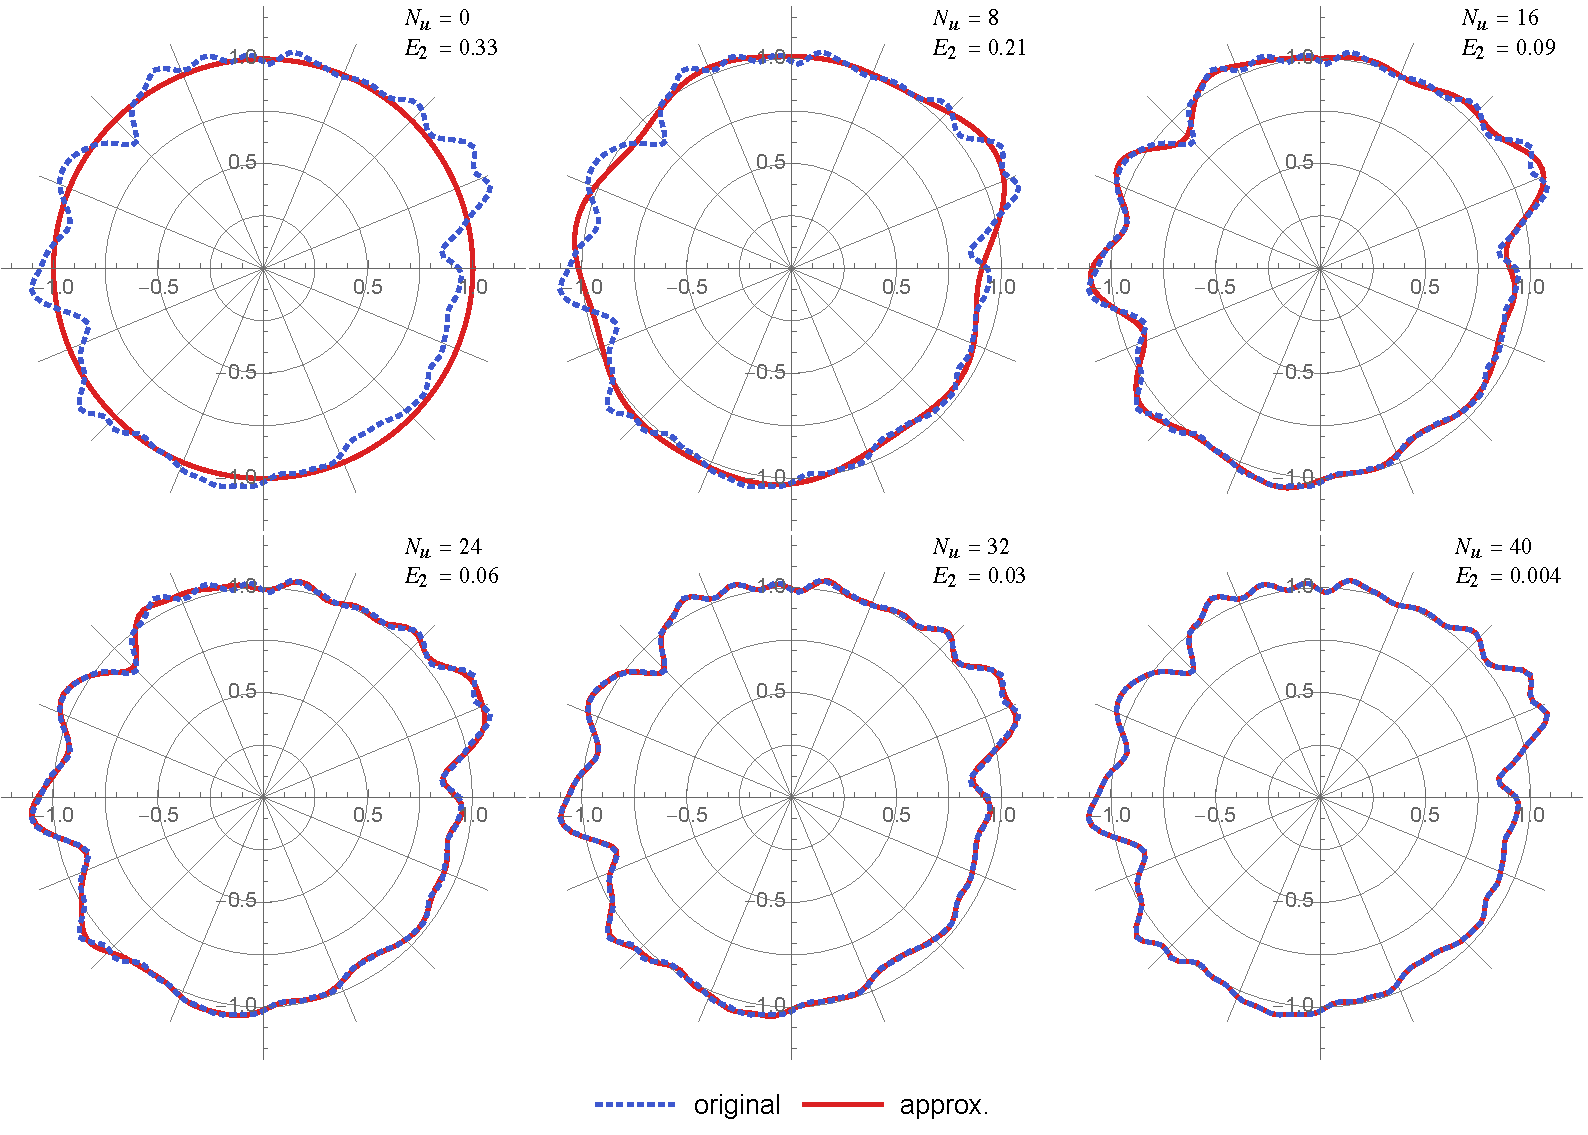
\includegraphics[width=.9\textwidth]{fig/equator/fourier.pdf}
  \caption{Fourier series approximations of displacement norms 
  on the Gauss-Lobatto-Legendre (GLL) points distributed along the outer edge of Fig.~\ref{fig:3deq},
  or the equatorial great circle indicated in Fig.~\ref{fig:sk}. 
  $N_u$ represents the number of terms in the Fourier series 
  and $E_2$ the $L^2$ norm of fitting error. We use  
  Discrete Fourier Transform (DFT) to compute Fourier coefficients, 
  and then inverse DFT to compute approximated distributions 
  after truncating the Fourier series at different $N_u$'s.} 
  \label{fig:four}
\end{figure*}

\subsection{Spectral properties of 3-D models}
Two factors contribute to the azimuthal smoothness (small $N_u$) of 
a global seismic wavefield: axial singularity of a seismic point source 
and lateral smoothness of global tomographic models.  
In a source-centered coordinate system, the Fourier expansion 
of a seismic moment tensor only contains the first three terms 
($\alpha=0,\pm1,\pm2$), owing to the coordinate singularity 
of the axis, as explained in Section~\ref{sec:moment}.
For 1-D Earth models, these three terms respectively
excite monopole, dipole and quadrupole radiation patterns
\cite[]{nissen2007axisem, van2014seismic}, which means $N_u=2$ throughout 
the entire domain. In the above numerical example, the Fourier expansion of
the moment tensor only contains the zeroth order term $M_{rr}$, 
so only the monopole (rotation invariant) radiation pattern is excited 
and thus $N_u=0$.

Theoretically, $N_u$ may become infinitely large for an arbitrary 3-D model 
due to lateral wave scattering. However, in the case of smooth 3-D structures, 
the lateral scattering effects are so weak that  
the wavefield tend to maintain smooth in the azimuthal direction, as
illustrated by Fig.~\ref{fig:snapshot}. 
So the question arises as to whether the Earth's mantle is 
smooth enough for these ideas to stand. 
The answer seems to be affirmative because
the predominance of long-wavelength heterogeneity in the mantle 
\cite[]{su1991predominance} has been well agreed among
most of the recent tomographic models based on different data 
sets and inversion techniques \cite[]{becker2002comparison}.
To confirm the answer, we shall now analyze the Fourier spectra of 
three models, s362ani \cite[]{kustowski2008s362ani}, 
s20rts \cite[]{ritsema1999s20rts} and 
s40rts \cite[]{ritsema2011s40rts}.

Consider the shear velocity perturbation $\delta v_{\text{s}}\left(r,\theta,\phi\right)$ 
($\delta v_{\text{sh}}$ for s362ani) normalized to the respective background model.  
Similar to \eqref{eq:demo}, we expand it in Fourier series as
\begin{equation}
  \delta v_{\text{s}}\left(r,\theta,\phi\right)=\sum_{|\gamma| \le n_v} 
  \delta v_{\text{s}}^\gamma\left(r,\theta\right)\exp\left(\mathbbm{i}\gamma\phi\right),
  \label{eq:fourv}
\end{equation}
where the coefficients $\delta v_{\text{s}}^\gamma$ are computed as
\begin{equation}
  \delta v_{\text{s}}^\gamma\left(r,\theta\right) = \frac{1}{2\pi}\int_{-\pi}^{\pi}
  \delta v_{\text{s}}\left(r,\theta,\phi\right)\exp\left(-\mathbbm{i}\gamma\phi\right)
  \text{d}\phi,
  \label{eq:invfourv}
\end{equation}
and $n_v$ denotes the Fourier spectral order required for a good approximation. 
Note that $n_v$ should be a field in the 2-D meridian domain, 
$n_v=n_v\left(r,\theta\right)$,
quantifying the local lateral smoothness of the model. 
Meanwhile, the maximum value of $n_v$ over the domain, denoted $N_v$, 
\begin{equation}
  N_v=\max_{r\in[0,R_{\text{earth}}],\ \theta\in[0,\pi]}n_v\left(r,\theta\right),
\end{equation} 
may serve as a global quantification. 
The spectral power associated with \eqref{eq:invfourv} is defined as
\begin{equation}
  \sigma_{\text{s}}^\gamma\left(r,\theta\right)=\frac{1}{\gamma+1} 
  \left|\delta v_{\text{s}}^\gamma\left(r,\theta\right) \right|^2.
  \label{eq:spow}
\end{equation}
Following \cite{becker2002comparison}, we normalize the spectral power by 
$\gamma+1$ to emphasize the wavelength dependence of heterogeneity. 

The conventional definition of a power spectrum is based on 
spherical harmonics expansion
\cite[]{su1991predominance, becker2002comparison} 
or, in a few cases, on Fourier expansion over a sphere-to-square map
\cite[]{chevrot1998spectrum}. In both cases, the spectral power spatially 
depends on depth only. In this paper, we need to define the power spectra
upon Fourier expansion over $\phi$, so the spectral 
power is a function of both $r$ and $\theta$, as indicated by \eqref{eq:spow}. 
It is also stressed that, because our Fourier expansion must be performed under 
the source-centered coordinate system, both the power spectrum and the field
of $n_v$ depend on the source location. Nevertheless, the global maximum 
order $N_v$ is source invariant, as it equals to the maximum degree 
$l_\text{max}$ of the corresponding spherical harmonics expansion. 
For instance, $N_v=20\ \text{and}\ 40$ 
respectively for s20rts and s40rts, parameterized horizontally 
by spherical harmonics, and $N_v=22$ for s362ani, parameterized by cubic 
splines both horizontally and vertically but with an equivalent lateral 
resolution of $l_\text{max}\approx 22$.

Given the model and a source, we first rotate the system such that 
the source lies on or beneath the north pole \cite[]{nissen2007axisem}. 
Then we compute $\delta v_{\text{s}}^\gamma$ by \eqref{eq:invfourv} and 
$\sigma_{\text{s}}^\gamma$ by \eqref{eq:spow}, for $\gamma=0,1,\dots$. 
Eventually, $n_v$ can be determined pointwise such that 
$\sigma_{\text{s}}^\gamma$ becomes negligibly small 
($<10^{-4}\sigma_{\text{s}}^0$) when $\gamma>n_v$. 
The results are shown in Fig.~\ref{fig:spectra}. As indicated by 
Fig.~\ref{fig:s3nv}-\ref{fig:s4nv}, the values of $N_v$ are as expected, 
i.e., $N_v=l_\text{max}$. The fields of $n_v$ are source dependent, but the 
governing pattern holds that $n_v\approx N_v\sin{\theta}$, divergence
from which reflects the nonuniformity of vertical resolution: e.g., a 
comparison between Fig.~\ref{fig:s3nv} and \ref{fig:s2nv} suggests that
s20rts has a more uniform vertical resolution while s362ani places more 
emphasis on the upper most mantle. Fig.~\ref{fig:s3pow}-\ref{fig:s4pow}
manifest concentrated spectral power on long wavelength modes with 
orders lower than 8, independent of source location.
In summary, small $N_v$'s as well as long-wavelength-focused power spectra 
verify the lateral smoothness of the tomographic models and thus 
imply the viability and efficiency of the Fourier spectral method.  

\begin{figure*}
  \centering
  \begin{minipage}{0.4\textwidth}
    \centering
    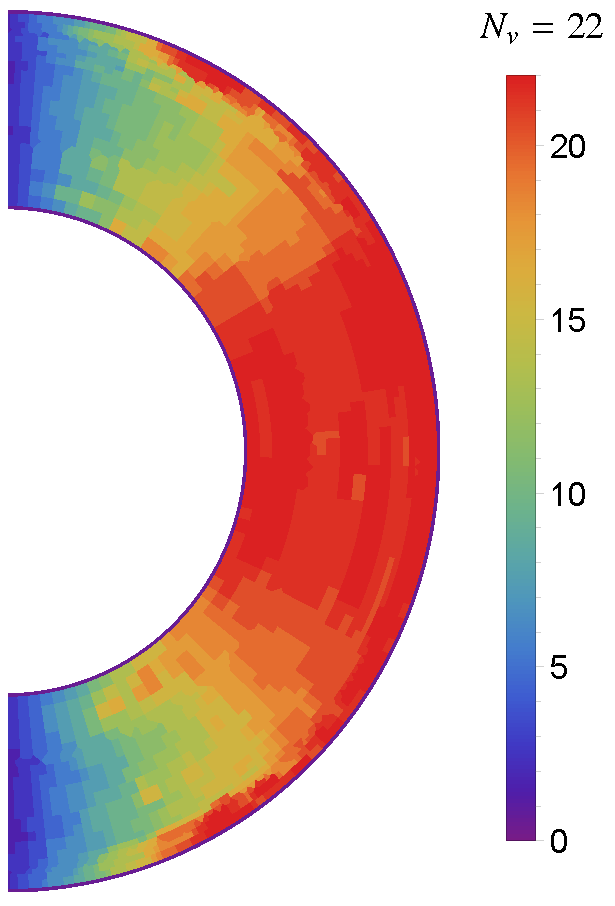
\includegraphics[height=.9\textwidth]{fig/model/s3nv.pdf} 
    \subcaption{$n_v$ of s362ani}
    \label{fig:s3nv}\par \medskip \vfill
    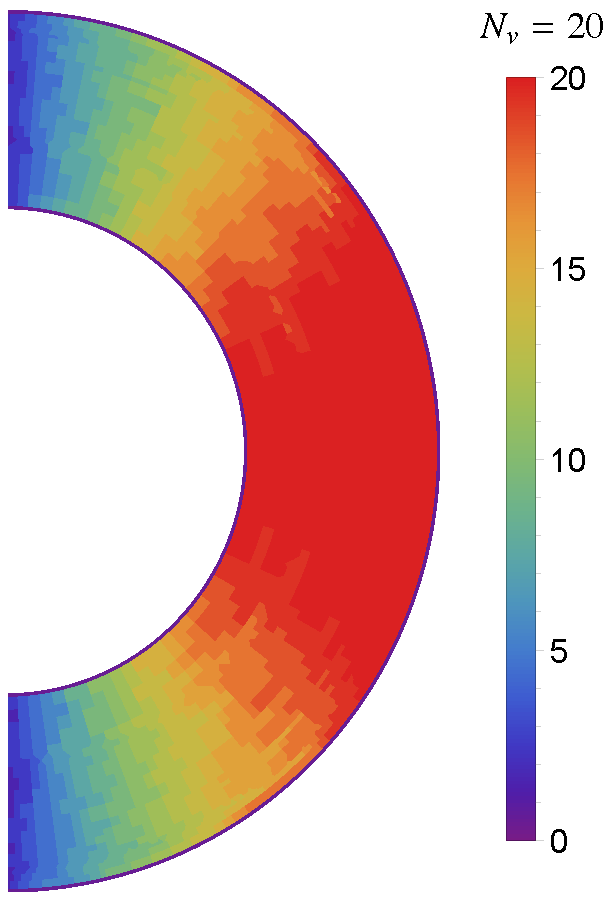
\includegraphics[height=.9\textwidth]{fig/model/s2nv.pdf} 
    \subcaption{$n_v$ of s20rts}
    \label{fig:s2nv}\par \medskip \vfill
    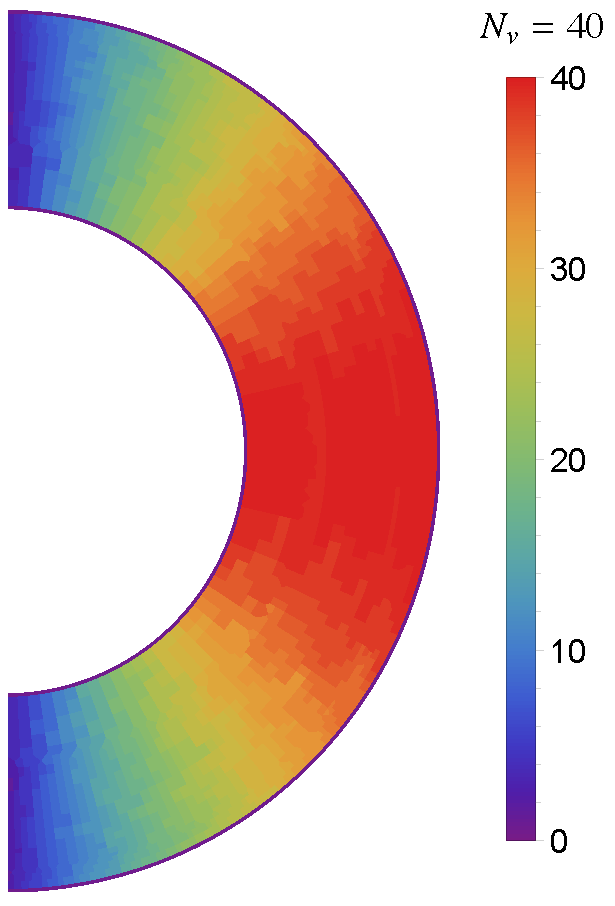
\includegraphics[height=.9\textwidth]{fig/model/s4nv.pdf} 
    \subcaption{$n_v$ of s40rts}
    \label{fig:s4nv}\par \medskip \vfill
  \end{minipage}%
  \begin{minipage}{0.6\textwidth}
    \centering
    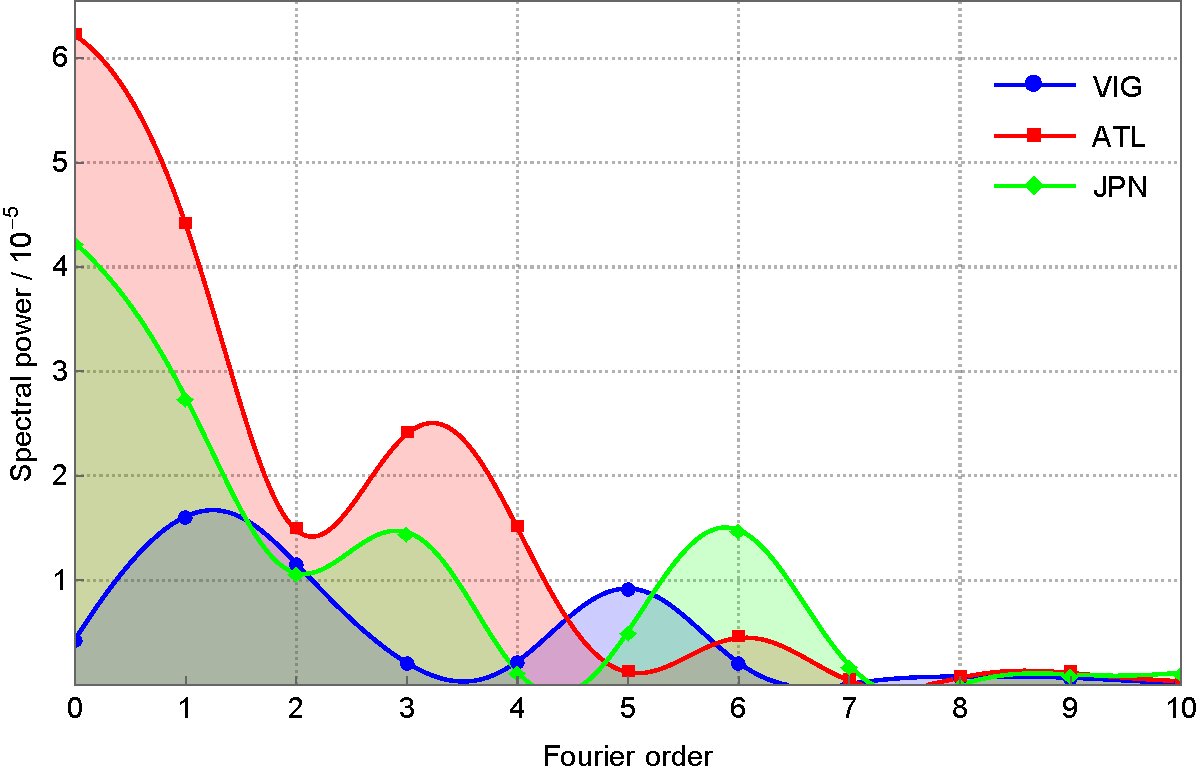
\includegraphics[height=.6\textwidth]{fig/model/s3pow.pdf} 
    \subcaption{spectral power of s362ani}
    \label{fig:s3pow}\par \medskip \vfill
    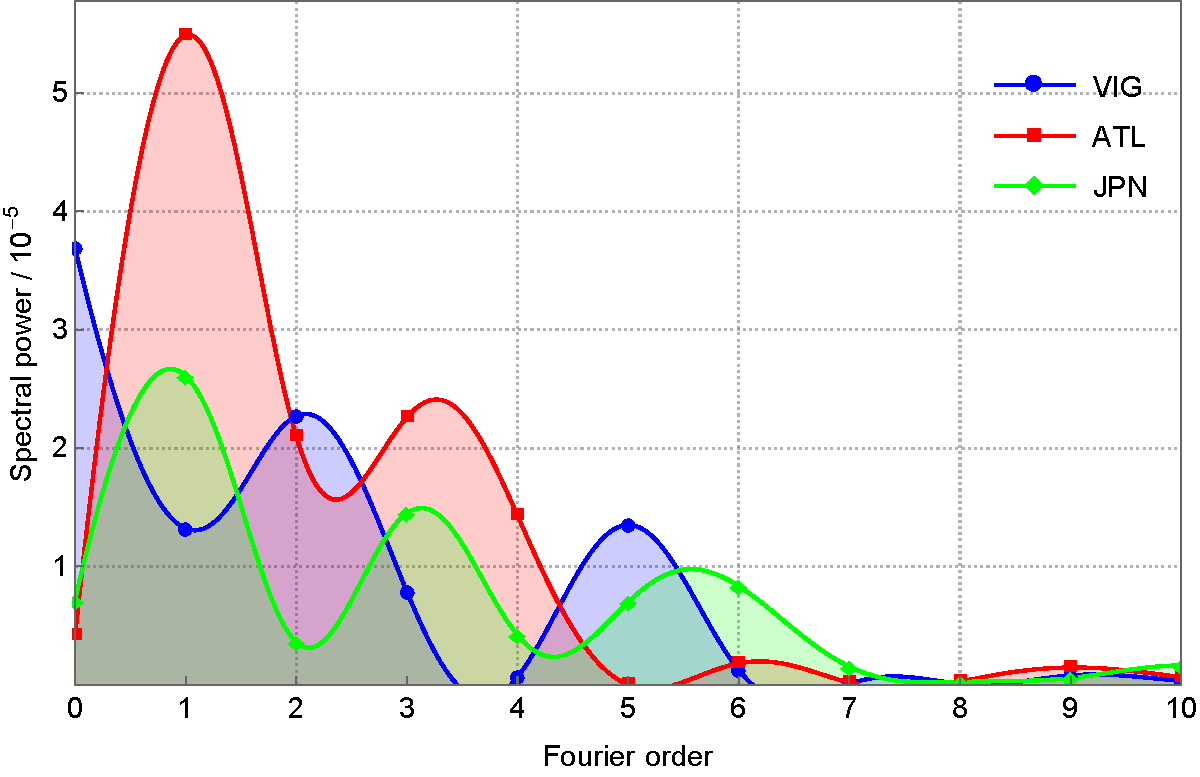
\includegraphics[height=.6\textwidth]{fig/model/s2pow.pdf} 
    \subcaption{spectral power of s20rts}
    \label{fig:s2pow}\par \medskip \vfill
    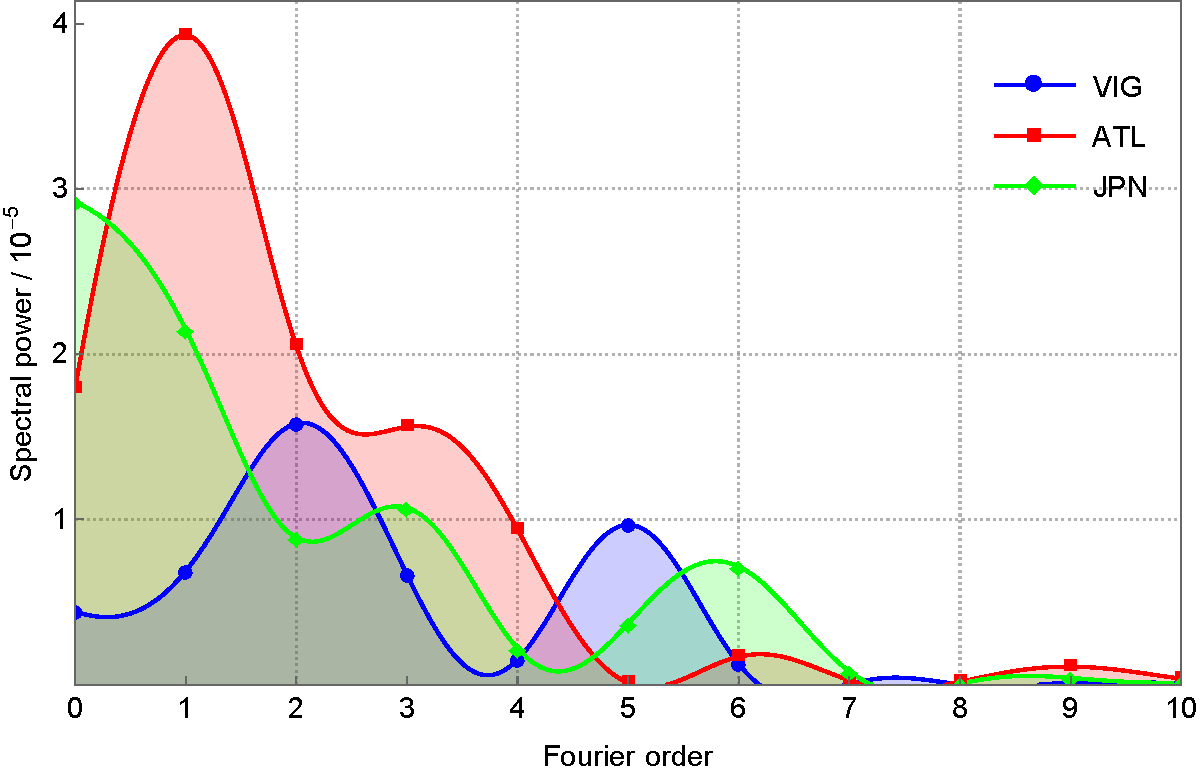
\includegraphics[height=.6\textwidth]{fig/model/s4pow.pdf} 
    \subcaption{spectral power of s40rts}
    \label{fig:s4pow}\par \medskip \vfill
  \end{minipage}%
  \caption{The $n_v$ fields and power spectra of three tomographic models.
  In (a)-(c), $n_v$ is determined such that $\sigma_{\text{s}}^\gamma$ 
  becomes negligibly small ($<10^{-4}\sigma_{\text{s}}^0$) when 
  $\gamma>n_v$ and $N_v$ the maximum $n_v$
  over the 2-D domain; 
  the source is located at VIR (37.91\degr N, 77.93\degr W, Virginia).
  (d)-(f) shows the power spectra at the point
  $\left(r,\theta\right)=\left(6291\text{km},90\degr\right)$, based on different source
  locations. Only the first 11 orders are plotted in view of vanishing 
  higher order values. Similar patterns can be found for other points 
  in the 2-D domain. 
  The source locations in (d)-(f) include: VIR (
  37.91\degr N, 77.93\degr W, Virginia), ATL (35.38\degr S, 
  16.40\degr W, southern mid-Atlantic ridge) and JPN (27.94\degr N, 
  140.56\degr E, Bonin Islands, Japan).}
  \label{fig:spectra}
\end{figure*}

\subsection{Method architecture}
\label{sec:idea}
Based on the above inspections of seismic wavefields upon 3-D Earth models, 
we propose a hybrid numerical method combining spectral element method and
pseudo-spectral method with Fourier-type basis functions. 
Here we outline the basic ideas and main features of our method.

Let the equations of motion be loosely written as 
\begin{equation}
  \mathscr{L}u=f,
  \label{eq:eomloose}
\end{equation}
where the operator $\mathscr{L}$, $\mathscr{L}=\mathscr{L}\left(r,\theta,\phi\right)$, 
is determined by the model's density and velocity fields, and $u$ and $f$
denote the time-dependent displacement and source term fields, respectively,
$u=u\left(r,\theta,\phi;t\right)$ and $f=f\left(r,\theta,\phi;t\right)$. 
We characterize the azimuthal dependences of functions
by Fourier series, see \eqref{eq:demo}, and 
\begin{align}
  & f\left(r,\theta,\phi;t\right)=\sum_{|\beta| \le N_f} 
  f^\beta\left(r,\theta;t\right)\exp\left(\mathbbm{i}\beta\phi\right),
  \label{eq:demof}\\[.5em]
  & \mathscr{L}\left(r,\theta,\phi\right)=\sum_{|\gamma| \le N_v} 
  \mathscr{L}^\gamma\left(r,\theta\right)\exp\left(\mathbbm{i}\gamma\phi\right).  
  \label{eq:demoL}
\end{align}
Note that we use ``$\simeq$'' for \eqref{eq:demo} but ``$=$'' for 
\eqref{eq:demof} and \eqref{eq:demoL} because the former is an 
assumption that holds in an asymptotic sense as $N_u\rightarrow\infty$,
whereas the latter two are exactly known a priori.  
The value of $N_f$ in \eqref{eq:demof} has been determined for all 
commonly used source types in seismology, e.g., 
2 for point source moment tensors, 
1 for point forces (used to compute the Fr\'echet kernels, 
see \cite{nissen2007axisem}) and 0 for explosions. 
Also note that $N_\rho$ does not appear in \eqref{eq:demoL} because we 
assume the density field to be smoother than the velocity field, i.e., 
$N_\rho \le N_v$, as is always the case in typical tomographic models. 

Instead of directly solving $u$ from $\mathscr{L}$ and $f$ in the 3-D
domain $\left(r,\theta,\phi\right)$, we attempt to solve the coefficients $u^\alpha$ from 
$\mathscr{L}^\gamma$ and $f^\beta$ in the 2-D meridian domain $\left(r,\theta\right)$. 
The general architecture of the method is shown in Fig.~\ref{fig:framework}. A 
critical step is to establish the relationship between $u^\alpha$ and
$\left(\mathscr{L}^\gamma,f^\beta\right)$, i.e., the dimension-reduced
equations of motion, as will be accomplished in Section~\ref{sec:theory}.

\begin{figure}
\setlength{\unitlength}{.0047\textwidth} 
\centering 
\begin{picture}(100,60) 
  \multiput(0,48)(4,0){25}{\line(1,0){3}}
  \multiput(0,34)(4,0){25}{\line(1,0){3}}
  \multiput(0,22)(4,0){25}{\line(1,0){3}}
  \multiput(0,8)(4,0){25}{\line(1,0){3}}
  \multiput(22,0)(0,4){15}{\line(0,1){3}}
  \multiput(43,0)(0,4){15}{\line(0,1){3}}
  \multiput(90,0)(0,4){15}{\line(0,1){3}}
  \multiput(70,0)(0,4){15}{\line(0,1){3}}
  
  \put(39,41){\line(1,0){36.5}}
  \put(39,40.5){\line(1,0){36.5}}
  \put(76,40.75){\vector(1,0){1}}
  \put(40,15){\vector(1,0){37}}
  \put(32.5,37){\vector(0,-1){18}}
  \put(80,19){\vector(0,1){18}}
  
  \put(28,40){{\fontsize{8pt}{1pt}\selectfont $\mathscr{L},f$}}
  \put(79,40){{\fontsize{8pt}{1pt}\selectfont $u$}}
  \put(50,43){{\fontsize{8pt}{1pt}\selectfont 3-D SEM}}
  \put(1,40){{\fontsize{8pt}{1pt}\selectfont 3-D domain}}
  \put(27,14){{\fontsize{8pt}{1pt}\selectfont $\mathscr{L}^\gamma,f^\beta$}}
  \put(79,14){{\fontsize{8pt}{1pt}\selectfont $u^\alpha$}}
  \put(50,17){{\fontsize{8pt}{1pt}\selectfont 2-D SEM}}
  \put(1,14){{\fontsize{8pt}{1pt}\selectfont 2-D domain}}
  \put(25,29){{\fontsize{8pt}{1pt}\selectfont FFT}}
  \put(25,25){{\fontsize{8pt}{1pt}\selectfont in $\phi$}}
  \put(82,29){{\fontsize{8pt}{1pt}\selectfont FFT}}
  \put(82,25){{\fontsize{8pt}{1pt}\selectfont in $\phi$}}
  \put(27,53){{\fontsize{8pt}{1pt}\selectfont knowns}}
  \put(73,53){{\fontsize{8pt}{1pt}\selectfont unknowns}}
\end{picture}
\caption{Architecture of the pseudo-spectral/spectral-element method. 
The double-lined arrow represents the workflow taken by full 3-D SEM, 
while our method follows the single-lined arrows. The Fast Fourier Transform (FFT)
on the left happens before time loop while the FFT on the right is required
only at the receivers, both of which take negligible computing time.} 
\label{fig:framework} 
\end{figure}  

Let us have a glance at the cost issue.
Let $\omega$ denote the dominant frequency of a simulation, or the highest 
frequency resolvable by the mesh. 
Combining theoretical (Section~\ref{sec:strong}) and numerical 
(Section~\ref{sec:benfreq} and \ref{sec:perf}) analysis, we shall demonstrate 
a cost of $O\left(N_v^q\omega^3\right)$ for our method, where 
$q$ is a positive real constant greater than 1.
First, the prefactor $N_v^q$ suggests that the cost of our method is 
model-dependent, distinct from full 3-D methods. 
Second, for a specific model, 
the cost of the method scales with $\omega^3$,
in comparison to $\omega^4$ for full 3-D methods,
which means our method should become \textit{increasingly} 
advantageous as $\omega$ increases and thus preferable for high 
frequency applications.  

%%%%%%%%%%%%%%%%%%%%%%%%%%%%%%%%%%%%%%%%%%%%%%%%%%%%%%%%%%%%%%%%%%%%%%%%%%%%%%%%
\section{Theory}
\label{sec:theory}
In this section, we derive the dimension-reduced equations of motion
on a 2-D meridian domain and investigate their computational characteristics.
For brevity, we shall exclude the fluid core and present the complete 
formulation for solid-fluid Earth models in Appendix~\ref{sec:fluid}.
Viscoelasticity based on standard linear solid model can be introduced 
straightforwardly following \cite{van2014optimized} and will not be
repeated here.    

%~~~~~~~~~~~~~~~~~~~~~~~~~~~~~~~~~~~~~~~~~~~~~~~~~~~~~
\subsection{Equations of motion in 3-D}
Consider an anisotropic elastic Earth model with spherical volume $\Omega$
and surface $\partial\Omega$. A point within $\Omega$ is referred
to by its position $\mathbf{r}$, and the unit outward normal
to $\partial\Omega$ is denoted $\hat{\mathbf{n}}$. 
Let $\mathbf{u}\left(\mathbf{r};t\right)$
and $\mathbf{f}\left(\mathbf{r};t\right)$ denote the time-dependent
fields of displacement and body force, respectively, 
and $\rho\left(\mathbf{r}\right)$
and $\mathbf{C}\left(\mathbf{r}\right)$ the fields of density and
fourth-order stiffness tensor, respectively. The 
time-dependent equations of motion may be written as
\begin{align}
  & \mathscr{L}\mathbf{u}=\mathbf{f},\ \text{in}\ \Omega,
  \label{eq:eom3d}\\[.5em]
  & \mathscr{B}\mathbf{u}=\mathbf{0},\ \text{on}\ \partial\Omega,
  \label{eq:surf3d}
\end{align}
where the operators are defined as
\begin{align}
  & \mathscr{L}\mathbf{u} \coloneqq \rho\ddot{\mathbf{u}}-
  \nabla\cdot\left(\mathbf{C}:\nabla\mathbf{u}\right),\\[.5em]
  & \mathscr{B}\mathbf{u} \coloneqq \hat{\mathbf{n}}\cdot
  \left(\mathbf{C}:\nabla\mathbf{u}\right),
\end{align}
with $\ddot{\mathbf{u}}$ standing for the second-order time 
derivative of $\mathbf{u}$.

The homogenous Neumann boundary condition \eqref{eq:surf3d} can be
efficiently handled by the following weak form 
\begin{equation}
  \langle \rho\ddot{\mathbf{u}},\mathbf{w}\rangle_{\Omega}+
  a_{\Omega}\left(\mathbf{u},\mathbf{w}\right)=\langle 
  \mathbf{f},\mathbf{w}\rangle_{\Omega}
  ,\ \forall\mathbf{w}\ \text{in}\ \Omega,
  \label{eq:3dweak}
\end{equation}
where $\mathbf{w}$, $\mathbf{w}=\mathbf{w}\left(\mathbf{r}\right)$, denotes an
arbitrary test function (it can be arbitrary only because no Dirichlet
boundary condition is present on the surface), and the inner product and 
bilinear form in $\Omega$ are defined respectively as
\begin{align}
  & \langle \mathbf{u},\mathbf{w}\rangle _{\Omega} \coloneqq
  \int_{\Omega}\mathbf{u}\cdot\mathbf{w}\,\text{d}^{3}\mathbf{r},\label{eq:3din}\\[.5em]
  & a_{\Omega}\left(\mathbf{u},\mathbf{w}\right) \coloneqq
  \int_{\Omega}\left(\nabla\mathbf{u}\right):\mathbf{C}:\left(\nabla\mathbf{w}\right)\text{d}^{3}\mathbf{r}.
  \label{eq:3dbi}
\end{align}

%~~~~~~~~~~~~~~~~~~~~~~~~~~~~~~~~~~~~~~~~~~~~~~~~~~~~~
\subsection{Axisymmetric geometry}
The dimension reduction demands axisymmetric geometry
of the Earth model, which means the 3-D domain $\Omega$
is invariant by rotation around an axis. 
If ellipticity is to be taken into account, the
axis must be chosen in coincidence with the Earth's
axis of rotation; otherwise, any axis across the center is acceptable. 
We denote the 2-D meridian domain of $\Omega$ by $D$,
as it is D-shaped. The boundary of $D$ contains two parts, the meridian
of $\partial\Omega$, denoted $\partial D$, and the axis of rotation
that does not have a 3-D counterpart, denoted $A$, as shown in 
Fig.~\ref{fig:crd}.

We shall employ a system of cylindrical coordinates $\left(s,\phi,z\right)$
or $\left(x_1,x_2,x_3\right)$, which is related to the geocentric spherical 
coordinates $\left(r,\theta,\phi\right)$ by
\begin{equation}
  s=r\sin\theta,\ z=r\cos\theta.
\end{equation}
We shall work under a unit cylindrical basis, denoted  
$\left(\hat{\mathbf{s}},\hat{\mathbf{\upphi}},\hat{\mathbf{z}}\right)$
or $\left(\hat{\mathbf{g}}_{1},\hat{\mathbf{g}}_{2},\hat{\mathbf{g}}_{3}\right)$, 
which can be linked to the constant Cartesian basis 
$\left(\hat{\mathbf{e}}_{1},\hat{\mathbf{e}}_{2},\hat{\mathbf{e}}_{3}\right)$ by
\begin{equation}
  \begin{cases}
    \hat{\mathbf{s}}=\hat{\mathbf{g}}_1=\hat{\mathbf{e}}_{1}\cos\phi 
    + \hat{\mathbf{e}}_{2}\sin\phi, \\
    \hat{\mathbf{\upphi}}=\hat{\mathbf{g}}_2=-\hat{\mathbf{e}}_{1}\sin\phi 
    + \hat{\mathbf{e}}_{2}\cos\phi, \\
    \hat{\mathbf{z}}=\hat{\mathbf{g}}_3=\hat{\mathbf{e}}_3.
  \end{cases}
\end{equation}
The gradient operator under such a frame can be written as
$\nabla=\hat{\mathbf{s}}\partial_{s}+
\frac{1}{s}\hat{\mathbf{\upphi}}\partial_{\phi}+
\hat{\mathbf{z}}\partial_{z}$.
Because $\partial_{\phi}\hat{\mathbf{s}}=\hat{\mathbf{\upphi}}$ and 
$\partial_{\phi}\hat{\mathbf{\upphi}}=-\hat{\mathbf{s}}$,
the gradient of a generic vector $\mathbf{v}$, 
$\mathbf{v}=v_{j}\hat{\mathbf{g}}_{j}$, can be shown to read
\begin{equation}
\nabla\mathbf{v}=\left[v_{j,i}+\left(\frac{1}{s}-1\right)\delta_{i2}v_{j,2}
-\frac{1}{s}\delta_{i2}\epsilon_{3jk}v_{k}\right]
\hat{\mathbf{g}}_{i}\hat{\mathbf{g}}_{j},
\label{eq:grad}
\end{equation}
where $\delta_{ij}$ denotes the Kronecker delta, $\epsilon_{ijk}$ the
Levi-Civita symbol and $v_{j,k}$ an abbreviation of $\partial_{x_k}v_j$.
The above index notation is non-standard (compared to covariant and
contravariant formulations) but effectively shortens tensorial
equations in the weighted Sobolev space measured by $s\,\text{d}s\,\text{d}z$ 
\cite[Chap 2,][]{bernardi1999spectral}. 
It is also obvious that the unit outward
normal to $\partial D$ is always perpendicular to $\hat{\mathbf{\upphi}}$,
i.e., $\hat{n}_{2}\equiv0$.

The axisymmetric geometry of $\Omega$ directly leads to the following integral
equality, serving as a key to reduce the azimuthal dimension, 
i.e., for any functions $g(\phi)$ and $h(s,z)$, 
\begin{equation}
\int_{\Omega}g(\phi)h(s,z)s\,\text{d}s \text{d}\phi \text{d}z=
\int_{-\pi}^{\pi}g(\phi)\,\text{d}\phi\int_{D}h(s,z)s\,\text{d}s\text{d}z.
\label{eq:ieq}
\end{equation}

\begin{figure}
  \centering
  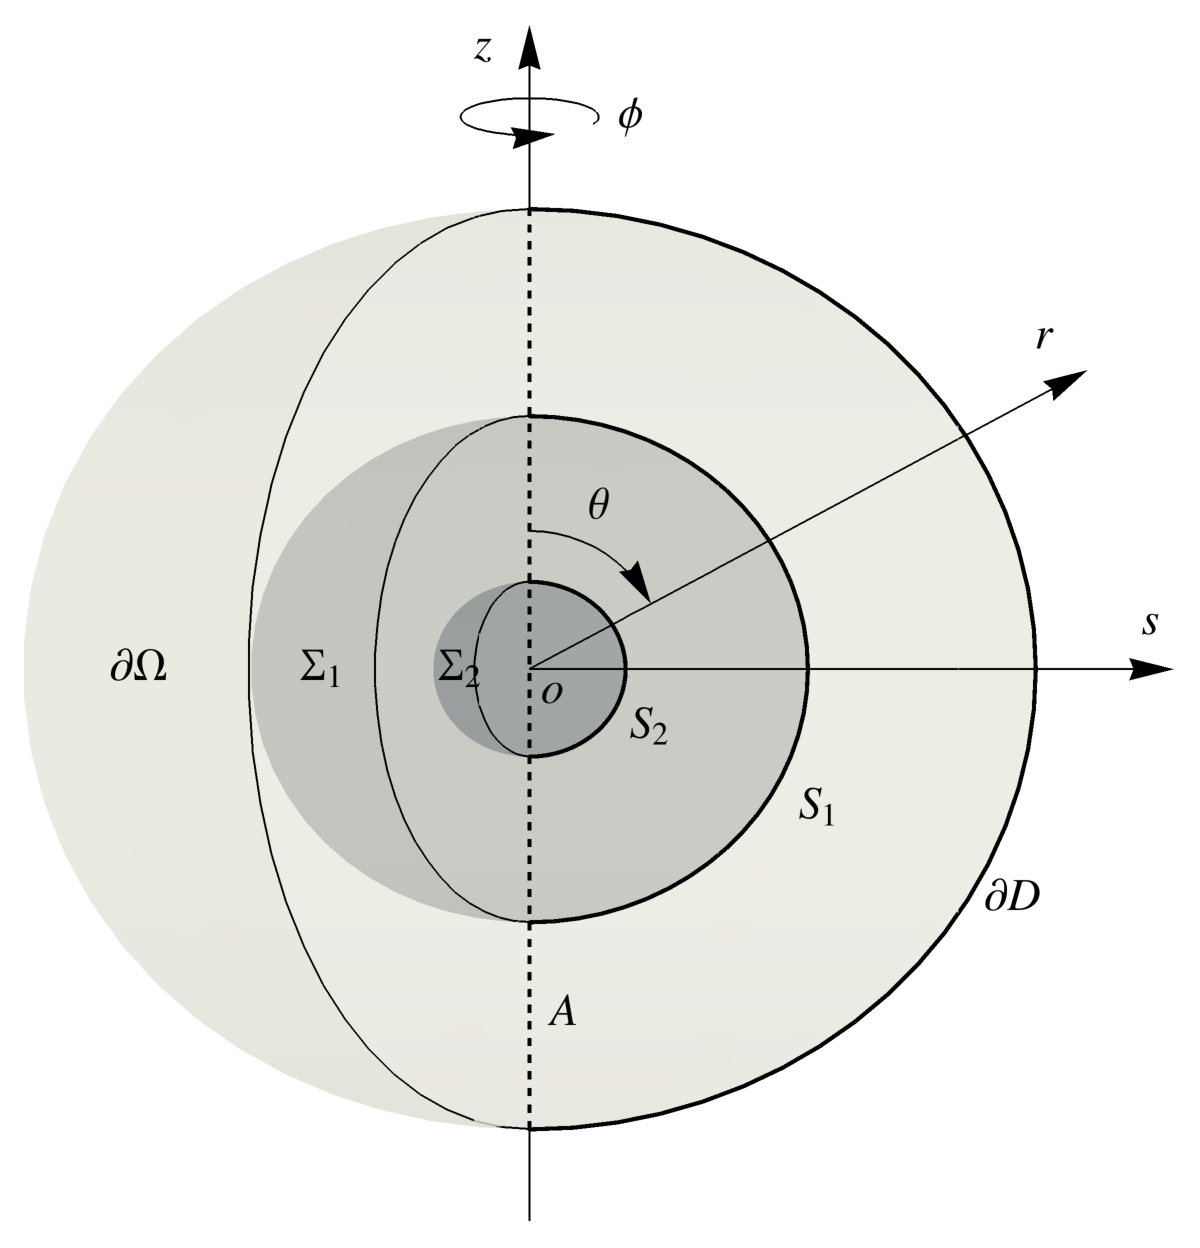
\includegraphics[width=.45\textwidth]{fig/theory/crd.pdf}
  \caption{Sketch of an Earth model with axisymmetric geometry. 
  The right-hand side shows the 2-D meridian domain $D$ with 
  physical boundaries $\partial D\cup S_i$ (thick curves) and 
  axial boundary $A$ (dashed thick line). $D$ is rotated about 
  the $z$-axis to generate the 3-D domain $\Omega$ with boundaries 
  $\partial\Omega\cup\Sigma_i$, as shown on the left-hand
  side. Here we denote the 3-D solid-fluid boundaries and 
  their 2-D meridians by $\Sigma_i$ and $S_i$, respectively, 
  which are not included in this section but later referred to in
  Appendix~\ref{sec:fluid}.}
\label{fig:crd}
\end{figure}

%~~~~~~~~~~~~~~~~~~~~~~~~~~~~~~~~~~~~~~~~~~~~~~~~~~~~~
\subsection{Dimension-reduced weak form}
Following the basic ideas in Section~\ref{sec:idea}, we characterize 
the azimuthal dependences of functions in terms of Fourier series,
i.e.%
\footnote{In this paper, Einstein summation convention applies to 
spatial indices such as $ijkl$ but not to Fourier indices such as
$\alpha\beta\gamma$.},
\begin{align}
  & \mathbf{u}=\hat{\mathbf{g}}_{i}\left(\phi\right) u_i\!\left(s,\phi,z;t\right) 
  \simeq \hat{\mathbf{g}}_{i}\left(\phi\right) \!\sum_{|\alpha|\le n_u} \!
  u_i^\alpha\!\left(s,z;t\right)\Psi^\alpha\left(\phi\right),
  \label{eq:u_four}\\[.5em]
  & \mathbf{f}=\hat{\mathbf{g}}_{i}\left(\phi\right) f_i\left(s,\phi,z;t\right) 
  = \hat{\mathbf{g}}_{i}\left(\phi\right) \!\sum_{|\alpha|\le n_f}\! 
  f_i^\alpha\left(s,z;t\right)\Psi^\alpha\left(\phi\right),
  \label{eq:f_four}\\[.5em]
  & \mathbf{w}=\hat{\mathbf{g}}_{i}\left(\phi\right) w_i\left(s,\phi,z\right) 
  = \hat{\mathbf{g}}_{i}\left(\phi\right) \sum_{|\beta|\le n_u} 
  w_i^\beta\left(s,z\right)\Psi^\beta\left(\phi\right),
  \label{eq:w_four}
\end{align}
where $\Psi^\alpha\left(\phi\right), \alpha=-n_u,\dots,n_u$ denote the Fourier modes, 
\begin{equation}
  \Psi^\alpha\left(\phi\right)\coloneqq\exp\left(\mathbbm{i}\alpha\phi\right),\ \mathbbm{i}=\sqrt{-1},
\end{equation}
which form an orthogonal set of basis functions,
\begin{equation}
  \int_{-\pi}^{\pi}\Psi^\alpha\left(\phi\right)\Psi^{-\beta}\left(\phi\right)\text{d}\phi=
  2\pi\delta_{\alpha\beta}.
  \label{eq:orth}
\end{equation}
Note that in \eqref{eq:w_four}, we construct the test space to coincide 
with the solution space by limiting $|\beta|\le n_u$, as necessitated by
the uniqueness of solution. Derivation of the source term
coefficients $f_i^\alpha$ will be elaborated in Section~\ref{sec:moment}.

The Fourier spectral order of solution, $n_u$, is a vital parameter 
because it defines the wavefield resolution in the $\phi$
direction and thus governs the computational cost. 
The azimuthal complexity of a wavefield is position dependent, 
e.g., near-axis regions demand much fewer orders than
far away from the axis. Hence, it is reasonable to assign 
$n_u$ locally, i.e., $n_u=n_u\left(s,z\right)$. The scheme to determine 
$n_u\left(s,z\right)$ will be elaborated in Section~\ref{sec:imp}. In the 
rest of the section, $n_u$ is treated as a constant, or one may
understand it as the global maximum order $N_u$. 
Such a notational simplification
does not affect generality of the theory. 

Substituted with \eqref{eq:u_four}, the displacement gradient 
\eqref{eq:grad} yields the following Fourier series form
\begin{equation}
  \nabla\mathbf{u}\simeq\hat{\mathbf{g}}_{i}\hat{\mathbf{g}}_{j}
  \sum_{|\alpha|\le n_u}u_{j;i}^\alpha\left(s,z;t\right) \Psi^\alpha\left(\phi\right),
  \label{eq:grad_u}
\end{equation}
where we define 
\begin{equation}
  u_{j;i}^\alpha \coloneqq u_{j,i}^\alpha+
  \frac{1}{s}\Gamma_{ijk}^\alpha u_k^\alpha,\quad 
  \Gamma_{ijk}^\alpha \coloneqq  
  \delta_{i2}\left(\mathbbm{i}\alpha\delta_{jk}-\epsilon_{3jk}\right),
  \label{eq:gamma}
\end{equation}
in view of that $u_{j,2}^\alpha \equiv 0$.
Here the role of $\Gamma_{ijk}^{\alpha}$ is quite similar to Christoffel
symbols in covariant and contravariant derivatives. 
Likewise, for the test function $\mathbf{w}$, we have
\begin{equation}
  \nabla\mathbf{w}=\hat{\mathbf{g}}_{i}\hat{\mathbf{g}}_{j}
  \sum_{|\beta|\le n_u}w_{j;i}^\beta\left(s,z\right) \Psi^\beta\left(\phi\right).
  \label{eq:grad_w}
\end{equation}

Substituting \eqref{eq:u_four}-\eqref{eq:w_four}, \eqref{eq:grad_u} and 
\eqref{eq:grad_w} into the 3-D weak form \eqref{eq:3dweak}, and 
applying the integral equality \eqref{eq:ieq} as well as the orthogonality condition
\eqref{eq:orth}, we eventually establish the weak form in the 2-D meridian 
domain $D$, with the $\phi$-dimension reduced (see 
Appendix~\ref{sec:dweak} for detailed derivation),
\begin{equation}
  \begin{alignedat}{1}
    & \sum_{|\alpha|\le n_u} \left[ 
    \left\langle \rho^{-\left(\alpha+\beta\right)}
    \ddot{\mathbf{u}}^\alpha,\mathbf{w}^\beta \right\rangle _{D}
    + a_D^{-\left(\alpha+\beta\right)}
    \left(\mathbf{u}^\alpha,\mathbf{w}^\beta\right)\right] \\&= 
    \left\langle \mathbf{f}^{-\beta},\mathbf{w}^\beta \right\rangle _{D},\quad
    \forall \mathbf{w}^\beta\ \text{in}\ D, \quad 
    \forall \beta\in \{-n_u,\dots,n_u\},
  \end{alignedat}
\label{eq:2dweak}
\end{equation}
where the inner product and bilinear form in $D$, in relation to 
\eqref{eq:3din} and \eqref{eq:3dbi}, are defined respectively as 
\begin{align}
  & \left\langle \mathbf{u}^\alpha,\mathbf{w}^\beta\right\rangle _{D}
  \coloneqq \int_D u_i^\alpha w_i^\beta s\,\text{d}s\text{d}z, \\[.5em]
  & a_D^\gamma \left(\mathbf{u}^\alpha,\mathbf{w}^\beta\right)\coloneqq
  \int_D u_{i;j}^\alpha C_{ijkl}^\gamma w_{k;l}^\beta s\,\text{d}s\text{d}z.
  \label{eq:bi}
\end{align}
The parameters involved in \eqref{eq:2dweak},
$\rho^\gamma$ and $C_{ijkl}^\gamma$, are respectively
the $\gamma$-th order Fourier coefficients of $\rho$ and $C_{ijkl}$, i.e.,
\begin{align}
  & \rho^\gamma\left(s,z\right)=
  \frac{1}{2\pi}\int_{-\pi}^{\pi}\rho\left(s,\phi,z\right)\Psi^{-\gamma}\left(\phi\right)\text{d}\phi,
  \label{eq:four_rho} \\[.5em]
  & C_{ijkl}^\gamma\left(s,z\right)=
  \frac{1}{2\pi}\int_{-\pi}^{\pi}C_{ijkl}\left(s,\phi,z\right)\Psi^{-\gamma}\left(\phi\right)\text{d}\phi,
  \label{eq:four_c}
\end{align}
or, inversely,
\begin{align}
  & \rho\left(s,\phi,z\right)=\sum_{|\gamma|\le n_\rho} 
  \rho^\gamma\left(s,z\right) \Psi^{\gamma}\left(\phi\right),
  \label{eq:ifour_rho} \\[.5em]
  & C_{ijkl}\left(s,\phi,z\right)=\sum_{|\gamma|\le n_c} 
  C_{ijkl}^\gamma\left(s,z\right) \Psi^{\gamma}\left(\phi\right).
  \label{eq:ifour_c}
\end{align}
where $n_\rho$ and $n_c$ are the maximum Fourier expansion orders 
required for an accurate description of the model, defined pointwise like $n_u$.
Apparently, for each term in \eqref{eq:2dweak}, summation of the 
superscripts always makes 0, as a result of 
the orthogonality condition \eqref{eq:orth}.

With $\beta$ evaluated between $[-n_u,n_u]$, Equation~\eqref{eq:2dweak} yields
$2n_u+1$ coupled weak forms to constrain the $2n_u+1$ Fourier coefficients 
$\mathbf{u}^\alpha$. We shall discuss the implementation of a 2-D SEM to solve
\eqref{eq:2dweak} in Section~\ref{sec:imp}. 
The structure of the dimension-reduced system is discussed in 
Section~\ref{sec:strong}, based on a more intuitive strong form
equivalent to \eqref{eq:2dweak}.   

\subsection{Axial boundary conditions}
Special attention must be paid to the axis $A$􏰁, a boundary of the 2-D 
computational domain $D$ that does not have a physical counterpart 
in the 3-D Earth model. The \textit{essential} boundary conditions on
$A$ are of Dirichlet type, which must be imposed on \eqref{eq:2dweak} 
explicitly to ensure the well-posedness of the Galerkin problem. 

If the functional form of the solution is analytically known, one may
derive the axial conditions directly by evaluating the asymptotic
behavior of the solution as $s\rightarrow0$ or $\theta\rightarrow0$, e.g., 
\cite{nissen2007axisem} from the normal-mode solution of 1-D models. 
We cannot follow this path because no analytical solution has been reported 
for 3-D models. Alternatively, one may impose the axial conditions such 
that the potential energy of the system is bounded, e.g.,
\cite{lopez1998efficient} and \cite{fournier2005fourier}. 
In fact, because the wavefield is globally continuous (except on 
solid-fluid boundaries), the boundedness of 
the potential energy is equivalent to the local boundedness of the 
displacement gradient, i.e., straight from \eqref{eq:gamma},
\begin{equation}
  \left(\mathbbm{i}\alpha\delta_{jk}-\epsilon_{3jk}\right) u_k^\alpha=0,\ j=1,2,3\quad,
  \label{eq:axbd}
\end{equation}
or 
\begin{equation}
  \begin{cases}
    u_s^0=u_\phi^0=0, & \alpha=0; \\
    u_s^1+\mathbbm{i}u_\phi^1=0,\ u_z^1=0, & \alpha=1; \\
    u_s^\alpha=u_\phi^\alpha=u_z^\alpha=0, & \alpha\ge2.
  \end{cases}
  \label{eq:mask}
\end{equation}
The result turns out to be identical to 1-D models \cite[]{nissen2007axisem}. 
Applying L'H\^opital's rule to \eqref{eq:gamma}, the displacement gradient 
at the axis turns into
\begin{equation}
  u_{j;i}^\alpha = u_{j,i}^\alpha+
  \Gamma_{ijk}^\alpha u_{k,1}^\alpha.
  \label{eq:axigrad_u}
\end{equation} 
  
%~~~~~~~~~~~~~~~~~~~~~~~~~~~~~~~~~~~~~~~~~~~~~~~~~~~~~
\subsection{Seismic moment tensor}
\label{sec:moment}
Now we evaluate the source term with respect to  
a time-dependent point source moment tensor $\mathbf{M}\left(t\right)$, 
positioned at $\mathbf{r}=\mathbf{r}_\text{s}$.  
The corresponding body force field can be written as
\begin{equation}
  \mathbf{f}\left(\mathbf{r};t\right)=
  -\mathbf{M}\left(t\right)\cdot\nabla\delta\left(\mathbf{r}-
  \mathbf{r}_{\text{s}}\right),
  \label{eq:f3d}
\end{equation}
where $\delta$ represents the Dirac-delta distribution. 
The right-hand side of the 3-D weak form \eqref{eq:3dweak} 
can then be written as
\begin{equation}
  \langle \mathbf{f},\mathbf{w}\rangle_{\Omega}=
  \mathbf{M}:  \nabla\mathbf{w}\left(\mathbf{r}_{\text{s}}\right).
  \label{eq:right3d}
\end{equation}

Note that for a point source, $\mathbf{M}$ in \eqref{eq:f3d} or 
\eqref{eq:right3d} is position-independent. 
Thus, its cylindrical components, $M_{ij}$, should depend on the $\phi$-coordinate, 
as the cylindrical basis vectors $\hat{\mathbf{g}}_{i}$ are $\phi$-dependent. 
To start from constant components, we first
represent $\mathbf{M}$ in the Cartesian coordinate system,
\begin{equation}
  \mathbf{M}=\hat{M}_{ij}\hat{\mathbf{e}}_{i}\hat{\mathbf{e}}_{j}.
\end{equation}
The cylindrical components $M_{ij}\left(\phi\right)$ can be linked to the constant 
Cartesian components $\hat{M}_{ij}$ 
by a rotation matrix $\mathbf{Q}\left(\phi\right)$, i.e.,
\begin{equation}
  \mathbf{M}=M_{ij}\hat{\mathbf{g}}_{i}\hat{\mathbf{g}}_{j},\quad 
  M_{ij}\left(\phi\right)=Q^\text{T}_{ik}\left(\phi\right)\hat{M}_{kl}Q_{lj}\left(\phi\right), 
  \label{eq:mij}
\end{equation}
where
\begin{equation}
  Q_{ij}\left(\phi\right) \coloneqq \hat{\mathbf{e}}_{i}\cdot\hat{\mathbf{g}}_{j} =
  \begin{bmatrix}
    \cos\phi & \sin\phi & 0 \\
    -\sin\phi & \cos\phi & 0 \\
    0 & 0 & 1
  \end{bmatrix}.
\end{equation}

Because the source azimuth $\phi_\text{s}$ becomes indeterminate on the axis, 
we consider axial and non-axial sources separately. 

\subsubsection{General sources}  
\label{sec:offaxis}
Substituted with \eqref{eq:mij} and \eqref{eq:grad_w}, 
\eqref{eq:right3d} yields 
\begin{equation}
  \langle \mathbf{f},\mathbf{w}\rangle_{\Omega}=
  M_{ij}\left(\phi_\text{s}\right)
  \sum_{|\beta|\le n_u} w_{i;j}^\beta\left(s_\text{s},z_\text{s}\right) 
  \Psi^\beta\left(\phi_\text{s}\right).
  \label{eq:na3d}
\end{equation}
As known from Appendix~\ref{sec:dweak}, the right-hand side of the 2-D weak 
form \eqref{eq:2dweak} can be derived from \eqref{eq:na3d} simply by 
scaling it with $\left(2\pi\right)^{-1}$ and dropping the summation over $\beta$, i.e., 
\begin{equation}
  \left\langle \mathbf{f}^{-\beta},\mathbf{w}^\beta \right\rangle _{D}=
  \frac{1}{2\pi}
  M_{ij}\left(\phi_\text{s}\right)
  w_{i;j}^\beta\left(s_\text{s},z_\text{s}\right) \Psi^\beta\left(\phi_\text{s}\right).
  \label{eq:na2d} 
\end{equation}
Without loss of generality, we assume $\phi_\text{s}=0$, and the above 
equation is simplified as
\begin{equation}
  \left\langle \mathbf{f}^{-\beta},\mathbf{w}^\beta \right\rangle _{D}=
  \frac{1}{2\pi}
  \hat{M}_{ij} w_{i;j}^\beta\left(s_\text{s},z_\text{s}\right). 
  \label{eq:na2da} 
\end{equation}

Equation~\eqref{eq:na2da} exposes an unfavorable fact that 
the reduced 2-D source term does not decay as $\beta$ increases. 
This is quite understandable because
the Dirac-delta distribution $\delta\left(\phi-\phi_\text{s}\right)$ involved in 
the 3-D source term has a white Fourier spectrum.
Therefore, no matter how large we choose the order $n_u$, we cannot 
model the source exactly, which causes uncontrollable errors that 
almost kill the numerical advantage of the pseudo-spectral methodology. 
Therefore, our method is currently inadequate for off-axis sources.

\subsubsection{Axial sources}
If the source is located on the axis, \eqref{eq:na2d} does not make sense
because $\phi_\text{s}$ becomes indeterminate when $s_\text{s}=0$. 
The axial source terms may be derived in various ways,
among which the simplest is from an asymptotic perspective.
Because the source can be imagined approaching 
to the axis from all azimuths, the axial source term 
should equal to the integration of \eqref{eq:na2d}
with respect to $\phi_\text{s}$ scaled by $\left(2\pi\right)^{-1}$, i.e., 
\begin{equation}
  \left\langle \mathbf{f}^{-\beta},\mathbf{w}^\beta \right\rangle _{D}
  = \frac{1}{2\pi}
  \hat{M}_{ij} \Lambda_{ijkl}^\beta w_{k;l}^\beta\left(0,z_\text{s}\right),
  \label{eq:ax2d} 
\end{equation}
where $\Lambda_{ijkl}^\beta$ is a constant fourth order tensor given by 
\begin{equation}
  \Lambda_{ijkl}^\beta=\frac{1}{2\pi}\int_{-\pi}^{\pi}
  Q_{ik}\left(\phi_\text{s}\right) Q_{jl}\left(\phi_\text{s}\right)
  \Psi^\beta\left(\phi_\text{s}\right) \text{d}\phi_\text{s}.
\end{equation}
Clearly, since $\mathbf{Q}$ only involves $\Psi^0$ and $\Psi^{\pm1}$,
in view of the orthogonality condition \eqref{eq:orth}, $\Lambda_{ijkl}^\beta$
should vanish if $|\beta|>2$. Thus, the seismic moment tensor can be 
\textit{exactly} described in the 2-D domain as long as $n_u\ge2$.  

With $\Lambda_{ijkl}^\beta$ evaluated respectively for $\beta=0,1,2$ and 
$w_{k;l}^\beta$ substituted by the axial formulation of displacement 
gradient \eqref{eq:axigrad_u}, the axial source term
\eqref{eq:ax2d} can be finally simplified as 
\begin{itemize}
  \item Monopole term ($\beta=0$):
  \begin{equation} 
    2\pi \left\langle \mathbf{f}^{0},\mathbf{w}^0 \right\rangle _{D}=
    \left(\hat{M}_{xx}+\hat{M}_{yy}\right)w_{s,s}^0+\hat{M}_{zz}w_{z,z}^0
    \label{eq:mono}
  \end{equation}
  \item Dipole term ($\beta=1$):
  \begin{equation} 
    2\pi \left\langle \mathbf{f}^{-1},\mathbf{w}^1 \right\rangle _{D}=
    \frac{\hat{M}_{xz}-\mathbbm{i}\hat{M}_{yz}}{2} 
    \left(w_{s,z}^1+\mathbbm{i}w_{\phi,z}^1\right)
    \label{eq:di}
  \end{equation}
  \item Quadrupole term ($\beta=2$):
  \begin{equation} 
    2\pi \left\langle \mathbf{f}^{-2},\mathbf{w}^2 \right\rangle _{D}=
    \left(\!\frac{\hat{M}_{yy}-\hat{M}_{xx}}{2}\!+\!\mathbbm{i}\hat{M}_{xy}\!\right) 
    \left(w_{s,s}^2+\mathbbm{i}w_{\phi,s}^2\right)
    \label{eq:quad}
  \end{equation}
\end{itemize}
In \eqref{eq:mono}-\eqref{eq:quad}, all $w_{k,l}^\beta$'s are evaluated at 
the source location $\left(0,z_\text{s}\right)$. 
The above results are equivalent to the trigonometric formulations of 
\cite{nissen2007axisem}.
As expected, \eqref{eq:mono}-\eqref{eq:quad} may also be expressed in terms of 
$\mathbf{f}$, i.e.,
\begin{itemize}
  \item Monopole term ($\beta=0$):
  \begin{equation} 
    -2\pi 
    \begin{bmatrix}
      f_s^0\\f_\phi^0\\f_z^0
    \end{bmatrix}
    =
    \begin{bmatrix}
      \left(\hat{M}_{xx}+\hat{M}_{yy}\right)\delta'\left(s\right)\delta\left(z-z_\text{s}\right)\\
      0\\
      \hat{M}_{zz}\delta\left(s\right)\delta'\left(z-z_\text{s}\right)
    \end{bmatrix}
    \label{eq:fmono}
  \end{equation}
  \item Dipole term ($\beta=1$):
  \begin{equation} 
    -2\pi 
    \begin{bmatrix}
      f_s^{-1}\\f_\phi^{-1}\\f_z^{-1}
    \end{bmatrix}
    =
    \frac{\hat{M}_{xz}-\mathbbm{i}\hat{M}_{yz}}{2}
    \delta\left(s\right)\delta'\left(z-z_\text{s}\right)
    \begin{bmatrix}
      1\\\mathbbm{i}\\0
    \end{bmatrix}
    \label{eq:fdi}
  \end{equation}
  \item Quadrupole term ($\beta=2$):
  \begin{equation} 
    -2\pi 
    \begin{bmatrix}
       f_s^{-2}\\f_\phi^{-2}\\f_z^{-2}
    \end{bmatrix}
    =
    \left(\!\frac{\hat{M}_{yy}-\hat{M}_{xx}}{2}\!+\!\mathbbm{i}\hat{M}_{xy}\!\right)
    \!\delta'\!\left(s\right) \delta\!\left(z\!-\!z_\text{s}\right)
    \!\begin{bmatrix}
      1\\\mathbbm{i}\\0
    \end{bmatrix}
    \label{eq:fquad}
  \end{equation}
\end{itemize}
where $\delta'$ denotes the ``derivative'' of Dirac-delta distribution. 
It is noteworthy that $\delta$ and $\delta'$ appear in $\mathbf{f}$ 
\textit{only} along the in-slice directions, $s$ and $z$, 
which essentially explains why the wavefields can be smooth in the 
azimuthal direction (e.g. Fig.~\ref{fig:1deq} and Fig.~\ref{fig:3deq})
while experiencing rather high in-slice complexity
(e.g. Fig.~\ref{fig:1dsl} and Fig.~\ref{fig:3dsl}). 

The source terms for $\beta=0,1,2$ are classified as monopole, 
dipole and quadrupole, respectively, based on 
their induced radiation patterns within an infinitesimal neighborhood 
of the source point. Such radiation patterns may be termed 
\textit{source patterns}, as they are intrinsic (model-independent) 
source properties determined by the moment tensor, 
similar to focal mechanisms, as summarized in Fig.~\ref{fig:source}. 
The global radiation patterns strictly follow 
the source patterns of the same angular order \cite[]{nissen2007axisem}
for 1-D models, but deviate from them for 3-D models to some degree.

\begin{figure}
  \centering
  \begin{minipage}{0.48\textwidth}
    \setlength{\unitlength}{.0055\textwidth}  
    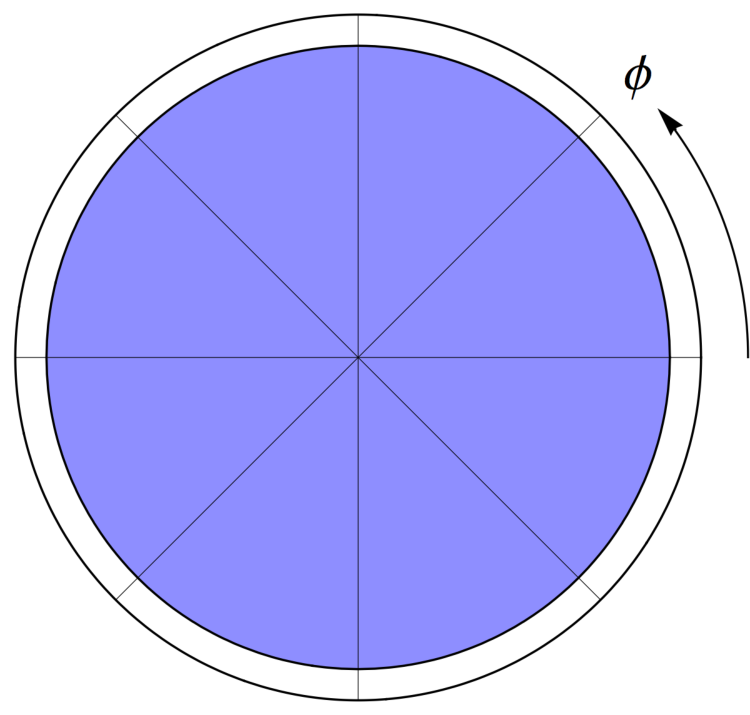
\includegraphics[width=.43\textwidth]{fig/source/mono.pdf}
    \begin{picture}(90,80)
      \put(10,57){{\fontsize{8pt}{1pt}\selectfont Monopole ($\beta=0$)}}
      \put(10,44){{\fontsize{8pt}{1pt}\selectfont Moment tensor elements}}
      \put(10,35){{\fontsize{8pt}{1pt}\selectfont $\hat{M}_{xx}+\hat{M}_{yy},\ \hat{M}_{zz}$}} 
      \put(10,22){{\fontsize{8pt}{1pt}\selectfont Source pattern}}
      \put(10,13){{\fontsize{8pt}{1pt}\selectfont $u_i\sim f\left(s,z\right)$}}
    \end{picture}
  \end{minipage}\\%
  \begin{minipage}{0.48\textwidth}
    \setlength{\unitlength}{.0055\textwidth}  
    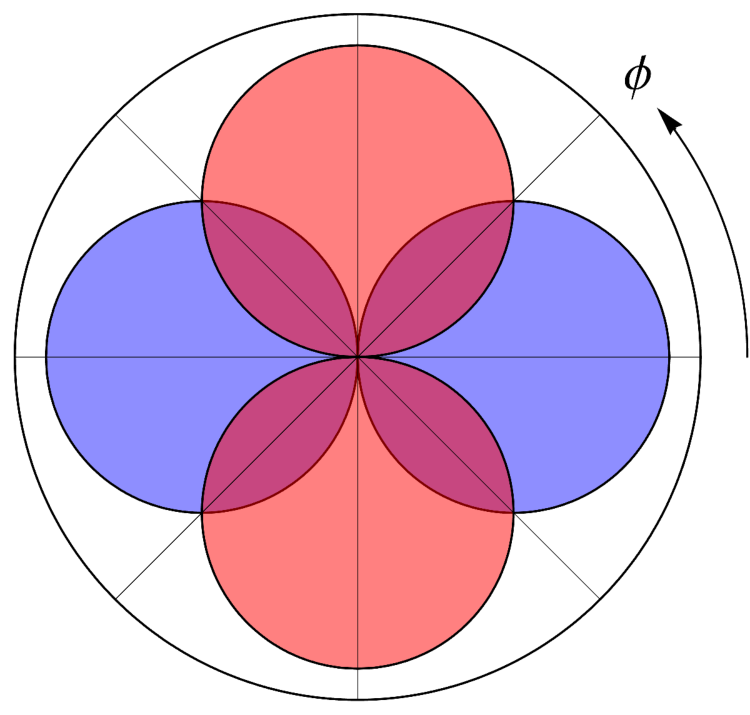
\includegraphics[width=.43\textwidth]{fig/source/di.pdf}
    \begin{picture}(90,80)
      \put(10,57){{\fontsize{8pt}{1pt}\selectfont Dipole ($\beta=\pm1$)}}
      \put(10,44){{\fontsize{8pt}{1pt}\selectfont Moment tensor elements}}
      \put(10,35){{\fontsize{8pt}{1pt}\selectfont $\hat{M}_{xz}-\mathbbm{i}\hat{M}_{yz}$}} 
      \put(10,22){{\fontsize{8pt}{1pt}\selectfont Source pattern}}
      \put(10,13){{\fontsize{8pt}{1pt}\selectfont $u_i\sim f\left(s,z\right)\cos\phi+g\left(s,z\right)\sin\phi$}}
    \end{picture}
  \end{minipage}\\%
  \begin{minipage}{0.48\textwidth}
    \setlength{\unitlength}{.0055\textwidth}  
    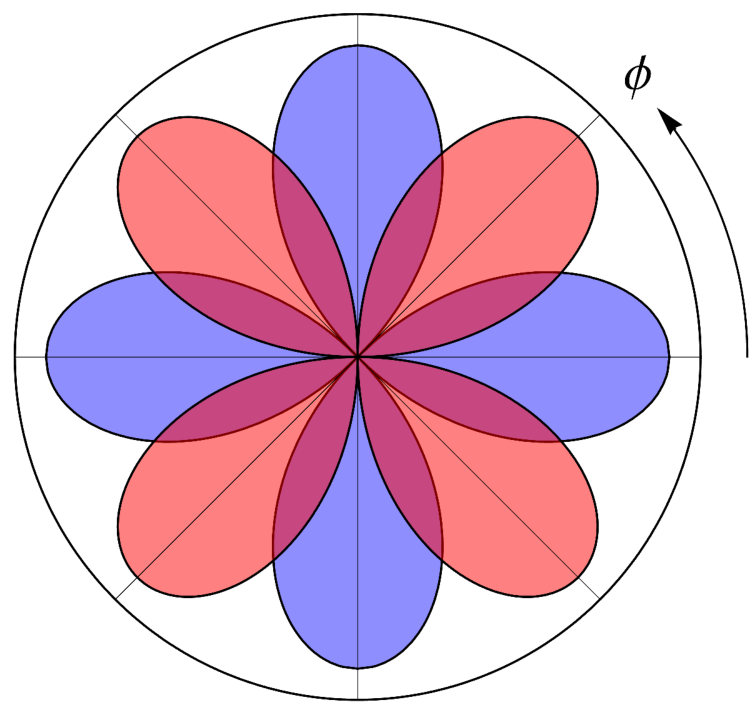
\includegraphics[width=.43\textwidth]{fig/source/quad.pdf}
    \begin{picture}(90,80)
      \put(10,57){{\fontsize{8pt}{1pt}\selectfont Quadrupole ($\beta=\pm2$)}}
      \put(10,44){{\fontsize{8pt}{1pt}\selectfont Moment tensor elements}}
      \put(10,35){{\fontsize{8pt}{1pt}\selectfont $\hat{M}_{yy}-\hat{M}_{xx}+2\mathbbm{i}\hat{M}_{xy}$}} 
      \put(10,22){{\fontsize{8pt}{1pt}\selectfont Source pattern}}
      \put(10,13){{\fontsize{8pt}{1pt}\selectfont $u_i\sim f\left(s,z\right)\cos 2\phi+g\left(s,z\right)\sin 2\phi$}}
    \end{picture}
  \end{minipage}
  \caption{Source patterns of an axial seismic moment tensor, 
  changed from \cite{nissen2014axisem}. 
  There are four distinct source patterns,
  two monopole (top), one dipole (middle) and one quadrupole. 
  For 1-D models, the source patterns also represent 
  the global radiation patterns.}
  \label{fig:source}
\end{figure}

%~~~~~~~~~~~~~~~~~~~~~~~~~~~~~~~~~~~~~~~~~~~~~~~~~~~~~
\subsection{Strong form and mode coupling}
\label{sec:strong}
The weak form \eqref{eq:2dweak} is efficient in handling the stress-free 
surface and convenient for SEM implementation, but the inherent structure 
of the dimension-reduced system is better revealed by an equivalent
strong form, as discussed below.

Applying the divergence theorem to \eqref{eq:2dweak}, recalling that 
$\hat{n}_{2}\equiv0$ and $u_{j,2}^\alpha \equiv 0$, we obtain the 
reduced strong form in correspondence to 
\eqref{eq:eom3d} and \eqref{eq:surf3d}, i.e.,
$\forall \beta\in \{-n_u,\dots,n_u\}$,
\begin{align}
  & \sum_{|\alpha|\le n_u}
  \mathscr{L}^{-\left(\alpha+\beta\right)}\mathbf{u}^\alpha=\mathbf{f}^{-\beta},
  \ \text{in}\ D,
  \label{eq:eom2d}\\[.5em]
  & \sum_{|\alpha|\le n_u}
  \mathscr{B}^{-\left(\alpha+\beta\right)}\mathbf{u}^\alpha=\mathbf{0},
  \ \text{on}\ \partial D,
  \label{eq:surf2d}
\end{align}
where the source terms $\mathbf{f}^{-\beta}$ are given by 
\eqref{eq:fmono}-\eqref{eq:fquad} for seismic moment tensors
and the reduced 2-D operators are defined as
\begin{align}
  & \mathscr{L}^{\gamma}\mathbf{u}^\alpha \coloneqq 
  \hat{\mathbf{g}}_i \left[
  \rho^\gamma \ddot{u}_i^\alpha-
  \left(C^\gamma_{ijkl} u_{k;l}^\alpha\right) _{;j}
  \right],
  \\[.5em]
  & \mathscr{B}^{\gamma}\mathbf{u}^\alpha \coloneqq 
  \hat{\mathbf{g}}_i \left[
  \hat{n}_j\left(C^\gamma_{ijkl} u_{k;l}^\alpha\right)
  \right].
\end{align}
Note that the surface tractions do not vanish on the axis $A$, but they do not  
have to be prescribed explicitly in \eqref{eq:surf2d} because $A$ is a Dirichlet 
boundary conditioned by \eqref{eq:axbd}.

Indeed, \eqref{eq:eom2d} defines a linear system of 2-D hyperbolic PDEs with 
a Hermitian \textit{Toeplitz} \cite[Chap 4,][]{golub2012matrix}
operator matrix of size $\left(2n_u+1\right)^2$, 
for instance, when $n_u=3$, 
\begin{equation}
  {\footnotesize
  \setlength{\arraycolsep}{3pt}
  \begin{bmatrix}\mathscr{L}^{0} & \mathscr{L}^{-1} & \mathscr{L}^{-2} & \mathscr{L}^{-3} & \mathscr{L}^{-4}& \mathscr{L}^{-5} & \mathscr{L}^{-6}\\
  \mathscr{L}^{1} & \mathscr{L}^{0} & \mathscr{L}^{-1} & \mathscr{L}^{-2} & \mathscr{L}^{-3}& \mathscr{L}^{-4} & \mathscr{L}^{-5}\\
  \mathscr{L}^{2} & \mathscr{L}^{1} & \mathscr{L}^{0} & \mathscr{L}^{-1} & \mathscr{L}^{-2}& \mathscr{L}^{-3} & \mathscr{L}^{-4}\\
  \mathscr{L}^{3} & \mathscr{L}^{2} & \mathscr{L}^{1} & \mathscr{L}^{0} & \mathscr{L}^{-1}& \mathscr{L}^{-2} & \mathscr{L}^{-3}\\
  \mathscr{L}^{4} & \mathscr{L}^{3} & \mathscr{L}^{2} & \mathscr{L}^{1} & \mathscr{L}^{0}& \mathscr{L}^{-1} & \mathscr{L}^{-2}\\
  \mathscr{L}^{5} & \mathscr{L}^{4} & \mathscr{L}^{3} & \mathscr{L}^{2} & \mathscr{L}^{1}& \mathscr{L}^{0} & \mathscr{L}^{-1}\\
  \mathscr{L}^{6} & \mathscr{L}^{5} & \mathscr{L}^{4} & \mathscr{L}^{3} & \mathscr{L}^{2}& \mathscr{L}^{1} & \mathscr{L}^{0}
  \end{bmatrix}\begin{bmatrix}
  \mathbf{u}^{-3}\\
  \mathbf{u}^{-2}\\
  \mathbf{u}^{-1}\\
  \mathbf{u}^{0}\\
  \mathbf{u}^{1}\\
  \mathbf{u}^{2}\\
  \mathbf{u}^{3}
  \end{bmatrix}=\begin{bmatrix}
  \mathbf{0}\\
  \mathbf{f}^{-2}\\
  \mathbf{f}^{-1}\\
  \mathbf{f}^{0}\\
  \mathbf{f}^{1}\\
  \mathbf{f}^{2}\\
  \mathbf{0}
  \end{bmatrix}}.
  \label{eq:full5}
\end{equation}
On the right-hand side, $\mathbf{f}^{-3}=\mathbf{f}^{3}=\mathbf{0}$,
because $n_f=2$ for a seismic moment tensor.
The non-diagonality of the operator matrix indicates the coupling of 
the Fourier modes. From the viewpoint of cardinal functions, the non-diagonal
operators ``scatter'' the wave energy from one slice to another.  
Such mode-coupling effects deserve utmost
care because it could deny the viability of the method if the 
computational cost surged with $n_u$.

For given resolution, let $N$ denote the number of grid points 
in a full 3-D mesh on the ring circle where $n_u$ is counted, 
e.g., both at the equatorial great circle.   
We have illustrated in Section~\ref{sec:snap} that $n_u \ll N$
for typical tomographic models, 
our initial motivation for the pseudo-spectral characterization. 
Nonetheless, \eqref{eq:eom2d} or \eqref{eq:full5} seems to suggest a 
computational complexity of $O\left(n_u^2\right)$ for the azimuthal dimension, 
in contrast to $O\left(N\right)$ for full 3-D methods. 
Fortunately, this is untrue for two reasons.

A well-known fact about a Toeplitz matrix $[\mathbf{T}]_{n\times n}$ 
is that the multiplication $[\mathbf{T}]_{n\times n}\{\mathbf{v}\}_n$ 
takes $O\left(n\log n\right)$ rather than $O\left(n^2\right)$ \cite[Chap 4,][]{golub2012matrix}. 
Thus, the azimuthal cost of the method can be reduced to 
$O\left(n_u\log n_u\right)$, i.e., the general cost of a pseudo-spectral method
subject to spatially-varying coefficients \cite[Chap 9,][]{boyd2001spectral}.
However, it still remains somewhat dissatisfactory 
because we desire $O\left(n_u\right)$ to ensure the advantage. 

What is not included in \eqref{eq:eom2d} is model complexity. 
Recalling \eqref{eq:ifour_rho} and \eqref{eq:ifour_c}, 
we note that $\rho^\gamma=0$ for $\gamma>n_\rho$ and 
$C_{ijkl}^\gamma=0$ for $\gamma>n_c$.
Therefore, the operator matrix is not only Hermitian Toeplitz 
but also banded, with a bandwidth of $\max\left(2n_c+1,2n_\rho+1\right)$. 
Based on our knowledge of Earth's nature, we assume $n_c\ge n_\rho$, 
and \eqref{eq:eom2d} turns into
\begin{equation}
  \sum_{\substack{|\alpha|\le n_u\\|\alpha+\beta|\le n_c}}
  \mathscr{L}^{-\left(\alpha+\beta\right)}\mathbf{u}^\alpha=\mathbf{f}^{-\beta},
  \ \text{in}\ D.
  \label{eq:band2d}
\end{equation}
For instance, when $n_c=1$, the example \eqref{eq:full5} reads
\begin{equation}
  {\footnotesize
  \setlength{\arraycolsep}{3pt}
  \begin{bmatrix}
  \mathscr{L}^{0} & \mathscr{L}^{-1} & 0 & 0 & 0 & 0 & 0\\
  \mathscr{L}^{1} & \mathscr{L}^{0} & \mathscr{L}^{-1} & 0 & 0 & 0 & 0\\
  0 & \mathscr{L}^{1} & \mathscr{L}^{0} & \mathscr{L}^{-1} & 0 & 0 & 0\\
  0 & 0 & \mathscr{L}^{1} & \mathscr{L}^{0} & \mathscr{L}^{-1} & 0 & 0\\
  0 & 0 & 0 & \mathscr{L}^{1} & \mathscr{L}^{0} & \mathscr{L}^{-1} & 0\\
  0 & 0 & 0 & 0 & \mathscr{L}^{1} & \mathscr{L}^{0} & \mathscr{L}^{-1}\\
  0 & 0 & 0 & 0 & 0 & \mathscr{L}^{1} & \mathscr{L}^{0}\\
  \end{bmatrix}\begin{bmatrix}
  \mathbf{u}^{-3}\\
  \mathbf{u}^{-2}\\
  \mathbf{u}^{-1}\\
  \mathbf{u}^{0}\\
  \mathbf{u}^{1}\\
  \mathbf{u}^{2}\\
  \mathbf{u}^{3}
  \end{bmatrix}=\begin{bmatrix}
  \mathbf{0}\\
  \mathbf{f}^{-2}\\
  \mathbf{f}^{-1}\\
  \mathbf{f}^{0}\\
  \mathbf{f}^{1}\\
  \mathbf{f}^{2}\\
  \mathbf{0}
  \end{bmatrix}}.
  \label{eq:band5}
\end{equation}
Apparently, the azimuthal cost further reduces to $O\left(n_c n_u\right)$ 
as long as $n_u \ge n_c$. In other words, the cost scales with $n_u$ 
for a specific model ($n_c=\text{const}$).
The condition $n_u \ge n_c$ can be easily achieved because $n_c$ has proved to
be small for typical tomographic models, as shown in Fig.~\ref{fig:spectra}. 

The banded structure also suggests a model-dependent computational cost. 
For models with smooth lateral variations (small $n_c$),  
the cost can be greatly lowered by a narrow bandwidth (weak mode coupling),
as well as its induced low complexity in the wavefield (small $n_u$).
We shall get back to this significant feature in more detail in 
Section~\ref{sec:adapt}, based on the computational costs observed from 
actual simulations.

%~~~~~~~~~~~~~~~~~~~~~~~~~~~~~~~~~~~~~~~~~~~~~~~~~~~~~
\subsection{Special case: 1-D models}
\label{sec:1d}
For spherically symmetric models, $n_c=n_\rho=0$, and the weak form \eqref{eq:2dweak} 
degenerates to
\begin{equation}
  \begin{alignedat}{1}
    & \left\langle \rho^{0}
    \ddot{\mathbf{u}}^{-\beta},\mathbf{w}^\beta \right\rangle _{D}
    + a_D^0
    \left(\mathbf{u}^{-\beta},\mathbf{w}^\beta\right)\\&= 
    \left\langle \mathbf{f}^{-\beta},\mathbf{w}^\beta \right\rangle _{D},\quad
    \forall \mathbf{w}^\beta\ \text{in}\ D, \quad 
    \beta=0,1,2
  \end{alignedat}\quad,
  \label{eq:1d}
\end{equation}
and the strong form \eqref{eq:eom2d} to 
\begin{equation}
  \mathscr{L}^0\mathbf{u}^{-\beta}=\mathbf{f}^{-\beta}, 
  \quad \text{in}\ D, \quad \beta=0,1,2.
\end{equation}
Evidently, the modes are fully decoupled in the 1-D case. 
Because the source term $\mathbf{f}^\beta$ vanishes for $\beta>2$,
as proved in Section~\ref{sec:moment}, we only need to consider 
the zeroth, first and second order modes, or the monopole, dipole 
and quadrupole radiation patterns, as shown in Fig.~\ref{fig:source}.
The weak form \eqref{eq:1d} epitomizes the results of 
\cite{nissen2007axisem} that lay the theoretical foundations
for the axisymmetric code AxiSEM \cite[]{nissen2014axisem}.


%%%%%%%%%%%%%%%%%%%%%%%%%%%%%%%%%%%%%%%%%%%%%%%%%%%%%%%%%%%%%%%%%%%%%%%%%%%%%%%%
\section{Implementation}
\label{sec:imp}
In this section, we briefly introduce the SEM implementation of the above
theory. Basically, we work by extending the 2-D spectral element code 
AxiSEM \cite[]{nissen2014axisem}, which has been established, tested
and improved via successive efforts of \cite{nissen2007sem, nissen2008sem,
van2014seismic, van2014optimized}. 
Most of the basic constituents remain unchanged for the 3-D extension,
such as spatial discretization, derivative and quadrature, and time-marching schemes.
Our 3-D implementation is named AxiSEM\_3D. 

\subsection{Spectral element discretization}
As shown in Fig.~\ref{fig:mesh}, the 2-D meridian domain is discretized 
by a finite element mesh, each element mapped onto a reference square 
on which all spatial operations take place. 
We use different types of geometric mapping 
($s=s\left(\xi,\eta\right)$ and $z=z\left(\xi,\eta\right)$)
for different regions of the mesh, such that the surface curvature can be
honored analytically \cite[]{nissen2007sem}.
Given the element shape, we can compute the elemental Jacobian
\begin{equation}
  \mathcal{J}\left(\xi,\eta\right)=\frac{\partial\left(s,z\right)}{\partial\left(\xi,\eta\right)}=\det 
  \begin{bmatrix}
    \partial_\xi s & \partial_\eta s \\
    \partial_\xi z & \partial_\eta z \\
  \end{bmatrix}.
  \label{eq:jacob}
\end{equation}
A generic function $f\left(s,z\right)$ on an element $D_\text{e}$ maps onto the 
reference square by $f\left(\xi,\eta\right)=f\left(s\left(\xi,\eta\right),z\left(\xi,\eta\right)\right)$, which is
approximated by the following piecewise interpolation,
\begin{equation}
  f\left(\xi,\eta\right)=f\left(s\left(\xi,\eta\right),z\left(\xi,\eta\right)\right) \approx 
  \sum_{\mathtt{p},\mathtt{q}=0}^{\mathtt{N}}
  f_{\mathtt{p}\mathtt{q}} l_{\mathtt{p}}^{\mathtt{N}}\left(\xi\right) 
  l_{\mathtt{q}}^{\mathtt{N}}\left(\eta\right),
\end{equation} 
where $f_{\mathtt{p}\mathtt{q}}$ is the value on the Gauss-Lobatto-Legendre
(GLL) point $\left(\xi_\mathtt{p},\eta_\mathtt{q}\right)$,
i.e., $f_{\mathtt{p}\mathtt{q}} = f\left(\xi_\mathtt{p},\eta_\mathtt{q}\right)$,
and $l_{\mathtt{p}}^{\mathtt{N}}$
the $\mathtt{p}$-th Lagrange interpolating function of polynomial order
$\mathtt{N}$, such that 
$l_{\mathtt{p}}^{\mathtt{N}}\left(\xi_\mathtt{q}\right)=
l_{\mathtt{p}}^{\mathtt{N}}\left(\eta_\mathtt{q}\right)=\delta_{\mathtt{p}\mathtt{q}}$ 
(diagonal mass matrix). 
Spatial derivatives of $f\left(s\left(\xi,\eta\right),z\left(\xi,\eta\right)\right)$ can then be computed as 
\begin{align}
 & \frac{\partial f}{\partial s} \approx 
 \sum_{\mathtt{p},\mathtt{q}=0}^{\mathtt{N}}
 \!\left[\frac{\partial z}{\partial \eta} 
 \frac{\partial l_{\mathtt{p}}^{\mathtt{N}}\left(\xi\right)}{\partial \xi}
 l_{\mathtt{q}}^{\mathtt{N}}\left(\eta\right)-  
 \frac{\partial z}{\partial \xi} 
 l_{\mathtt{p}}^{\mathtt{N}}\left(\eta\right)
 \frac{\partial l_{\mathtt{q}}^{\mathtt{N}}\left(\eta\right)}{\partial \eta}
 \right]\!f_{\mathtt{p}\mathtt{q}}\mathcal{J}^{-1},\label{eq:der}\\[.5em]
 & \frac{\partial f}{\partial z} \approx 
 \sum_{\mathtt{p},\mathtt{q}=0}^{\mathtt{N}}
 \!\left[\frac{\partial s}{\partial \xi} 
 l_{\mathtt{p}}^{\mathtt{N}}\left(\eta\right)
 \frac{\partial l_{\mathtt{q}}^{\mathtt{N}}\left(\eta\right)}{\partial \eta}
 -\frac{\partial s}{\partial \eta} 
 \frac{\partial l_{\mathtt{p}}^{\mathtt{N}}\left(\xi\right)}{\partial \xi}
 l_{\mathtt{q}}^{\mathtt{N}}\left(\eta\right)
 \right]\!f_{\mathtt{p}\mathtt{q}}\mathcal{J}^{-1}.\label{eq:der2}
\end{align}
The integral of $f\left(s\left(\xi,\eta\right),z\left(\xi,\eta\right)\right)$ over the element 
$D_\text{e}$ can be realized by the GLL quadrature
\begin{equation}
  \int_{D_\text{e}}f\left(s,z\right)s\,\text{d}s\text{d}z\approx 
  \sum_{\mathtt{p},\mathtt{q}=0}^{\mathtt{N}}
  \sigma_{\mathtt{p}}^{\mathtt{N}} \sigma_{\mathtt{q}}^{\mathtt{N}}
  s\left(\xi_\mathtt{p},\eta_\mathtt{q}\right) f_{\mathtt{p}\mathtt{q}}
  \mathcal{J}\left(\xi_\mathtt{p},\eta_\mathtt{q}\right),
  \label{eq:int}
\end{equation} 
where the weights are determined by 
$\sigma_{\mathtt{p,q}}^{\mathtt{N}}=
\int_{-1}^1 l_{\mathtt{p,q}}^{\mathtt{N}}\left(\xi\right)\text{d}\xi$.  
Note that \eqref{eq:der}-\eqref{eq:int} have to be modified to 
Gauss-Lobatto-Jacobi forms for the axial 
elements \cite[]{nissen2007sem} to handle the singularity $s=0$.

Equations \eqref{eq:jacob}-\eqref{eq:int} fulfill
the requirements for the spatial discretization of the 
dimension-reduced weak form \eqref{eq:2dweak}. 
For instance, the discretization of the stiffness term \eqref{eq:bi} 
follows the steps below:
\begin{enumerate}
  \item given the Fourier coefficients of displacement 
  $u_i^\alpha$, $-n_u\le\alpha\le n_u$, 
  on the GLL points of element $D_\text{e}$, compute the deformation gradient 
  $u_{i;j}^\alpha$ by \eqref{eq:gamma},
  where the derivatives $u_{i,j}^\alpha$ are evaluated 
  by \eqref{eq:der} and \eqref{eq:der2}; 
  \item compute the Fourier coefficients of stress pointwise, i.e., $\sigma_{kl}^\beta=
  \sum_{|\alpha|\le n_u}C_{ijkl}^{-\left(\alpha+\beta\right)} u_{i;j}^\alpha$, 
  for all $\beta=-n_u,\dots, n_u$; Mode coupling takes place in this step;
  \item similar to (i), compute the deformation gradient (denoted $\varsigma_{kl}^\beta$) with respect to 
  a discretized delta function $w_k^\beta$ that equals to 1 in the $x$-direction  
  ($x=s,\phi,z$) at a GLL point $P$ and vanishes otherwise; 
  \item compute the contraction $\sigma_{kl}^\beta \varsigma_{kl}^\beta$ pointwise
  and then its elemental integral by means of the quadrature \eqref{eq:int}; 
  The result yields the $\beta$-th order Fourier coefficient of the
  stiffness term in the $x$-direction at the GLL point $P$,
  contributed by element $D_\text{e}$; 
  \item assemble the elemental stiffness terms at shared GLL points to compute
  the global stiffness terms.
\end{enumerate}
In practice, the above process can be facilitated by a variety of 
properties and techniques, such as the sparsity of $C_{ijkl}$,
Hermitian of the reduced system and pre-computable terms. 

For the complete implementation, we refer the reader to \cite{nissen2007sem} 
(isotropic media) or \cite{van2014seismic} (anisotropic media),
where the implementation of \eqref{eq:1d}, i.e.,
the degenerated form of \eqref{eq:2dweak} for 1-D Earth models,
is elaborated. The 3-D generalizations are purely algebraic, basically
nothing but adding an outer loop of Fourier spectral orders when evaluating the
field variables. Such simplicity largely relies on
an explicit time scheme (and thus a diagonal mass matrix) that preserves 
the fundamental framework.  

\begin{figure}
  \centering
  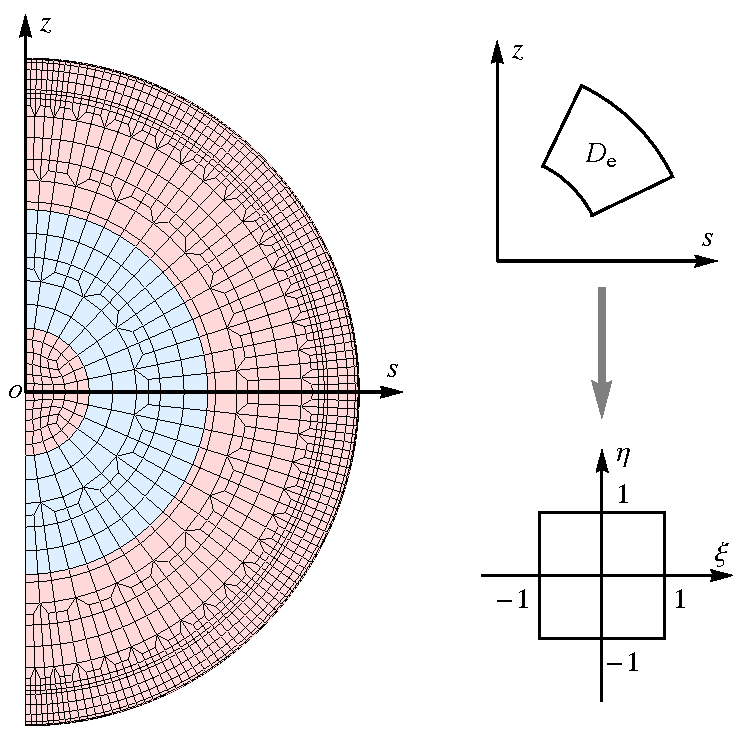
\includegraphics[width=.43\textwidth]{fig/mesh/mesh.pdf}
  \caption{Mesh architecture and geometric mapping. 
  In this example, the 2-D meridian domain $D$ is discretized by
  a mesh with 128 elements on the outer surface, the equal
  of $\mathtt{NEX}$ = 64 in SPECFEM (see \cite{carrington2008high} 
  for details of the SPECFEM parameter $\mathtt{NEX}$).
  Each element is mapped onto a reference square spanning 
  $-1\le \xi,\eta \le 1$, 
  on which all spatial operations take place.} 
  \label{fig:mesh}
\end{figure}

\subsection{Fourier spectral order of solution}
The most important issue of the 3-D extension is how to construct the field  
$n_u=n_u\left(s,z\right)$, namely, the maximum expansion order prescribed pointwise on
the Fourier characterization of solution, see \eqref{eq:u_four}. 
Apparently, $n_u\left(s,z\right)$ should increase with the local
azimuthal complexity of the wavefield, which is unknown before simulation. 
An optimized $n_u\left(s,z\right)$ may be determined via several trial 
simulations at some low frequency. However, one has to repeat 
the procedure once the model or the source location changes.
Hence, such a strategy appears impractical from a user's perspective.

Here we propose an empirical equation to determine 
a semi-optimized $n_u\left(s,z\right)$ dependent on position only, based on
a large number of low-frequency simulations using different tomography 
models and source locations. The empirical equation reads
\begin{equation}
  n_u=\max\left(\lceil n_u^\text{ref} F_s F_\theta F_d\rceil, n_u^\text{min}\right),
  \label{eq:nu}
\end{equation}
where $n_u^\text{ref}$ and $n_u^\text{min}$ denote respectively 
a basic reference value and the global minimum value, the only
two parameters from users, whereas $F_s$, $F_\theta$ and $F_d$
are three scale factors acting on $n_u^\text{ref}$ 
for different purposes, and the brackets $\lceil\ \rceil$ mean rounding 
up to the next integer.
Factor $F_s$ simply reflects the fact that points away from the axis 
should demand higher orders (more slices) than those close to the axis 
(note that $n_u\equiv 1$ on the axis, see \eqref{eq:mask}),  
\begin{equation}
  F_s=F_s\left(s\right)=\frac{s}{R_\text{earth}}.
  \label{eq:fs}
\end{equation}
Factor $F_\theta$ increases $n_u$ by the epicentral distance $\theta$,
since the further the waves travel, the more 3-D structures they ``see'',
\begin{equation}
  F_\theta=F_\theta\left(\theta\right)=
  \begin{dcases}
    1,&\theta\le\frac{\pi}{4};\\
    1+4\left(\frac{4\theta-\pi}{3\pi}\right)^3,&
    \frac{\pi}{4}<\theta\le\pi.
  \end{dcases}
  \label{eq:ft}
\end{equation}
Lastly, factor $F_d$ enhances the resolution of surface waves, 
\begin{equation}
  F_d=F_d\left(d\right)=
  \begin{dcases}
    2, & d \le d_{0}; \\
    4-2\frac{d}{d_{0}}, 
    &d_{0}<d\le1.5d_{0};\\
    1,& d > 1.5 d_{0},
  \end{dcases}
  \label{eq:fd}
\end{equation}
where $d$ denotes the depth, $d=R_\text{earth}-r$,
and $d_{0}$ a characteristic depth specifying 
the enhanced range, which must be considerably
greater than the penetration depth of the longest wavelength 
of interest. For a safe play, we choose $d_{0}=200\text{km}$.
Note that such enhancement will not increase the computational
cost much because it only affects a small fraction of elements. 
It is numerically found that one may set $F_d=1$ for deep 
earthquakes.

The constants in \eqref{eq:fs}-\eqref{eq:fd} may be adjusted 
for specific applications, e.g., doubling $F_d$ for a higher 
surface wave resolution. But, in general, one can simply
increase/decrease $n_u^\text{ref}$ for better accuracy/performance.

Fig.~\ref{fig:nu} shows examples of \eqref{eq:nu} where 
$n_u^\text{ref}=24$ and $n_u^\text{min}=8$, 
with and without surface wave enhancement. 
Mapping Fig.~\ref{fig:nu} onto Fig.~\ref{fig:mesh}, we obtain
the corresponding $n_u$ fields defined on a discretized mesh.
Note that $n_u$ is an indicator of computational cost,
which means the elemental cost should vary from element to element.
Before propagating waves, we may pre-examine the distributions of number of elements 
with respect to their Fourier spectral orders, e.g. Fig.~\ref{fig:count}, from which 
the relative performance for different choices of $n_u\left(s,z\right)$
 can be roughly estimated.
For instance, Fig.~\ref{fig:count} indicates that the surface wave 
enhancement by \eqref{eq:fd} primarily doubles the order of  
$\sim$20\% elements, and thus is less likely to produce a cost surge.

\begin{figure}
  \centering
  \begin{minipage}{0.22\textwidth}
    \centering
    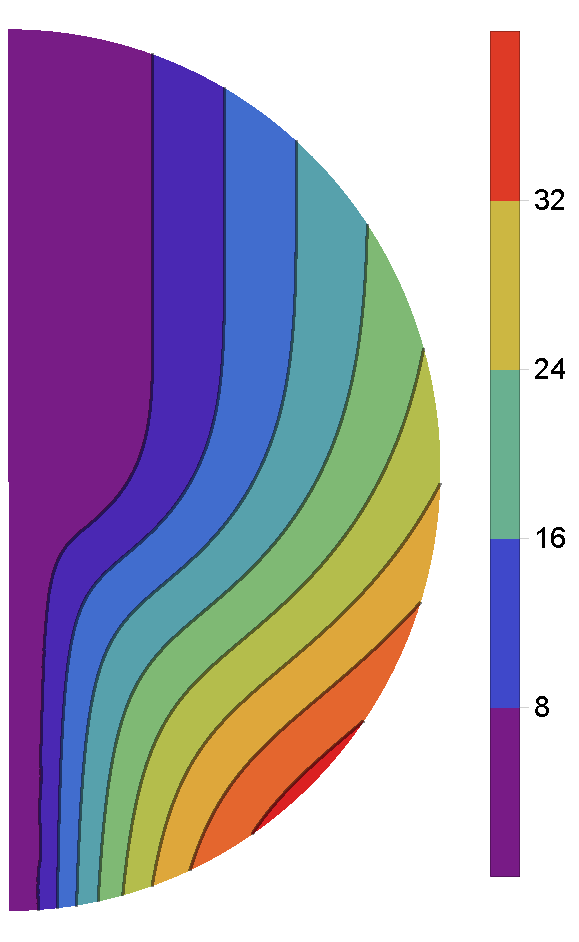
\includegraphics[width=\textwidth]{fig/nu24/ns.pdf}
    \subcaption{surface wave not enhanced}
  \end{minipage}\quad\quad\ %
  \begin{minipage}{0.22\textwidth}
    \centering
    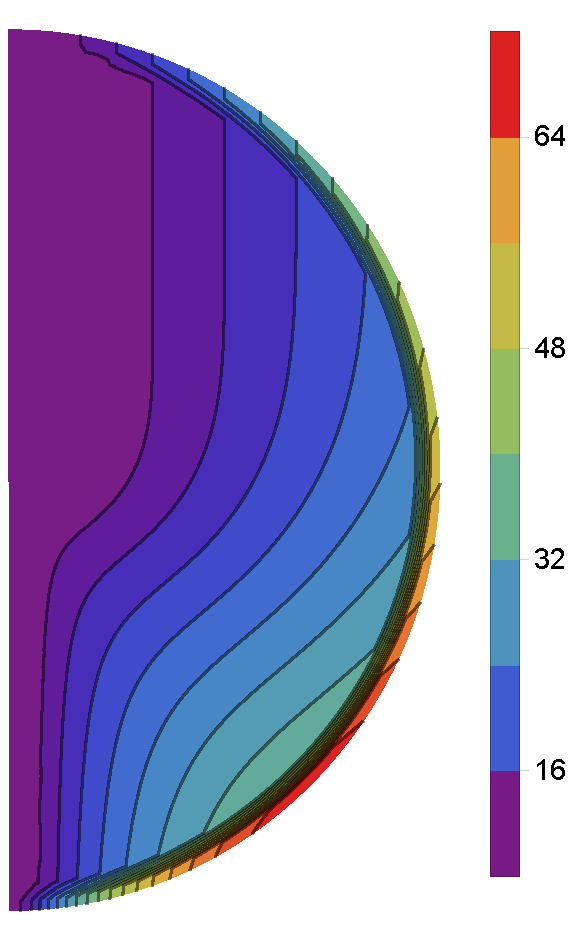
\includegraphics[width=\textwidth]{fig/nu24/ys.pdf}
    \subcaption{surface wave enhanced}
  \end{minipage}
  \caption{Examples of $n_u\left(s,z\right)$ fields, computed by 
  \eqref{eq:nu} with $n_u^\text{ref}=24$ and $n_u^\text{min}=8$. 
  The maximum value appears near $\theta=135\degr$ on the surface,
  a combined effect of $F_s$ and $F_\theta$. For deep earthquakes or 
  the cases where surface waves are not of interest, one may use (a); 
  otherwise, (b) should be employed to enhance surface wave resolution.
  Integer rounding ($\lceil\ \rceil$) is ignored in 
  the plots for a clearer view.} 
  \label{fig:nu}
\end{figure}

\begin{figure}
  \centering
  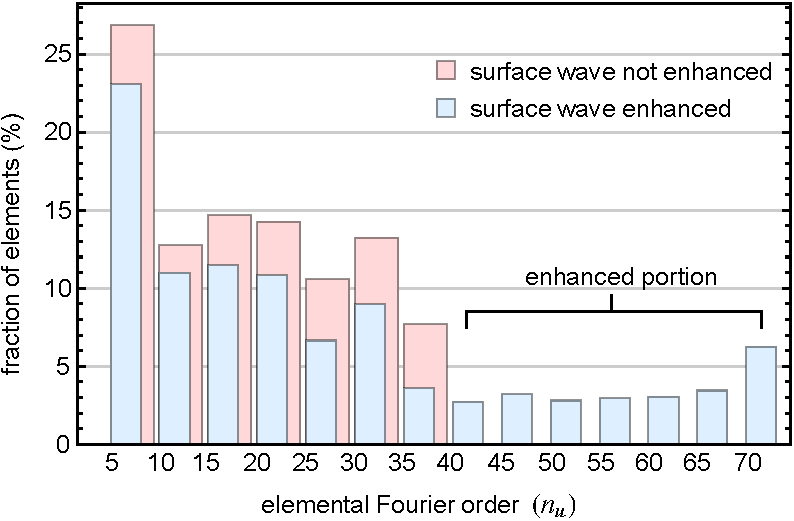
\includegraphics[width=.46\textwidth]{fig/elecnt/elecnt.pdf}
  \caption{Examples of element distributions with respect to elemental 
  Fourier spectral order. The statistics are based on the two $n_u$ fields shown in Fig.~\ref{fig:nu},
  with and without surface wave enhancement, which are mapped onto the mesh
  shown in Fig.~\ref{fig:mesh}. 
  The surface wave enhancement primarily doubles the order of  
  $\sim$20\% elements.} 
  \label{fig:count}
\end{figure}

\subsection{Stability}
Numerical stability could be another problem around the 3-D extension.
The stability of the axisymmetric method has been 
comprehensively considered for 1-D Earth models, 
\cite[]{nissen2008sem}, with special attention paid to the thin 
crustal layers, the internal discontinuities and the fluid outer core.
When extended to 3-D, the stability conditions generally become harsher.
Though the complete theory has remained an open question for 
general 3-D media \cite[]{gottlieb2001spectral}, we benefit 
from the smoothness of lateral heterogeneity, especially 
the absence of horizontal discontinuities,
allowing us to follow the 1-D conditions exactly
\cite[]{gottlieb2001spectral, gottlieb1981stability}. Numerical
applications show that time intervals determined by 1-D 
reference models still work well for 3-D tomographic models.
Note that time-stepping also serves as a small source of computational 
advantage, because the Courant number can be slightly larger 
in 2-D than in 3-D \cite[]{komatitsch1998spectral}.
 
 
%%%%%%%%%%%%%%%%%%%%%%%%%%%%%%%%%%%%%%%%%%%%%%%%%%%%%%%%%%%%%%%%%%%%%%%%%%%%%%%%
\section{Validation}
\label{sec:ben}
In this section, we benchmark AxiSEM\_3D in reference to 
a full 3-D SEM called SPECFEM3D\_GLOBE 
\cite[SPECFEM,][]{komatitsch2002spectralI,komatitsch2002spectralII}. 
We use the global tomographic model s362ani \cite[]{kustowski2008s362ani}
for validation, considering anisotropy \cite[]{van2014seismic}
and attenuation \cite[]{van2014optimized} but, for the time being,
ignoring 3-D crustal structures and internal topography at depths 
$\sim$410km and $\sim$660km. 
We shall discuss 3-D crusts and internal topography in Section~\ref{sec:geo}. 
Notably, this section could be a novel cross-validation, 
as to the best of our knowledge SPECFEM has been
the only published code to compute global seismic wavefields in 
3-D tomographic models.  

To ensure global coverage, we distribute a fictitious network of receivers 
evenly on the surface in the source-centered coordinate system, 
spaced by 15\degr in the $\theta$-direction (epicentral distance) and 
45\degr in the $\phi$-direction (azimuth), containing 88 receivers in total. 
An example is shown in Fig.~\ref{fig:rec}.

\begin{figure}
  \centering 
  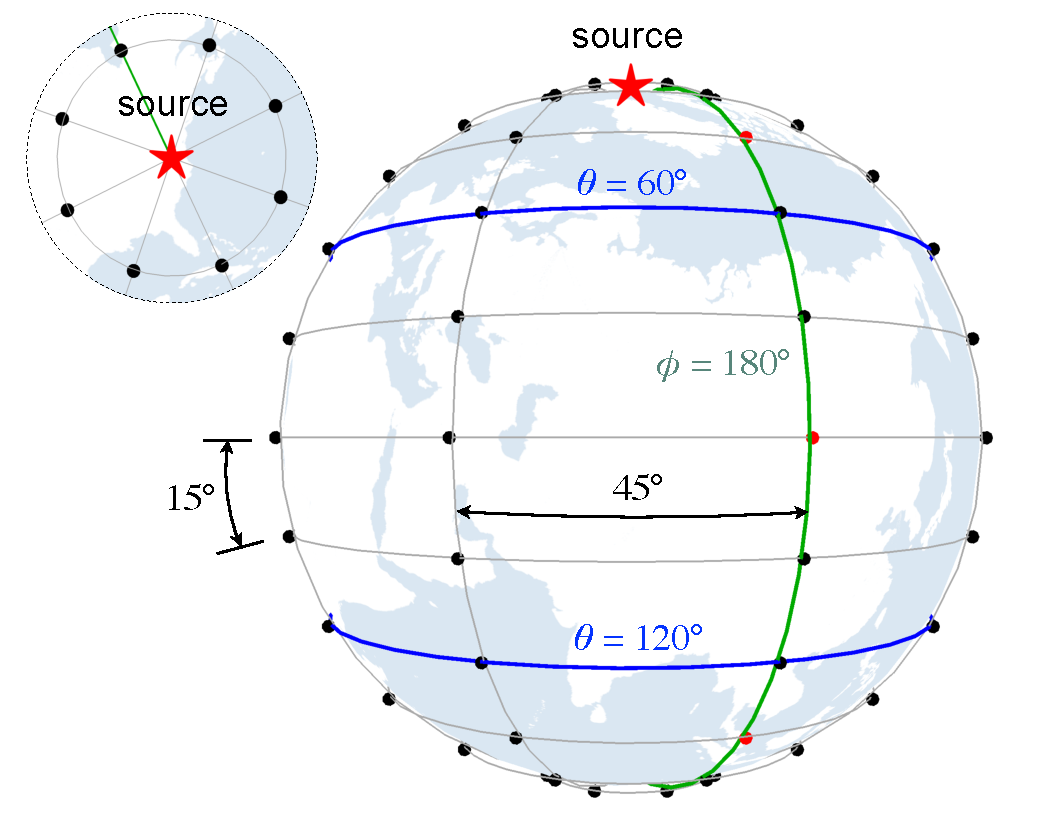
\includegraphics[width=.44\textwidth]{fig/rec/recev.pdf} 
  \caption{Source-centered receiver network. The source location 
  is VIR (37.91\degr N, 77.93\degr W, Virginia). 
  The colored dots and curves indicate the receivers 
  whose seismograms will be displayed later in this section
  to visualize benchmark results. We will focus on the meridian $\phi=180\degr$
  because most of its receivers are located on continents and the misfits 
  at this azimuth tend to be comparatively large. } 
  \label{fig:rec}
\end{figure}

The accuracy is quantified in terms of time-frequency misfits
\cite[TF-misfits,][]{kristekova2009time}. 
For each pair of synthetics (SPECFEM vs. AxiSEM\_3D), 
we compute the globally normalized 
envelope and phase misfits ($\mathtt{EM}$ and $\mathtt{PM}$) 
on three windows, the body wave governed window $[0,t_\text{surf}]$,
the surface wave governed window $[t_\text{surf},t_\text{max}]$ and 
the full-length window $[0,t_\text{max}]$, 
where $t_\text{surf}$ denotes an 
approximate travel time of the first surface wave arrival
and $t_\text{max}$ the length of the time series. 
We do not treat P-wave and S-wave separately because the accuracy
difference turns out to be insignificant.

Before accuracy judgement, an additional modification is applied to 
the TF-misfits. We compute synthetics for the corresponding
1-D reference model using both SPECFEM and AxiSEM 
\cite[the mature 1-D version,][]{nissen2014axisem} 
and then compute the 1-D misfits. 
We subtract the 1-D misfits from the 3-D ones, based on the fact
that the Fourier spectral theory holds exact for 1-D models, 
i.e., \eqref{eq:1d} is fully equivalent to \eqref{eq:3dweak}, 
and thus these 1-D misfits should result from purely numerical issues, 
such as distinct meshing schemes, source and receiver mislocations, and 
accumulative round-off errors.  
Indeed, the 1-D phase misfits turn out invariably small (\textless 2\%), 
but the envelope misfits might be comparatively large (up to 10\%)
on rare occasions for unidentified reasons. 

The results are deemed acceptable if the following three criteria are 
satisfied simultaneously: 
\begin{itemize}
  \item the global averages of the modified misfits over the receivers, 
  both envelope and phase, should not exceed 5\%;
  \item the local modified misfits should not exceed 10\% 
  (note that 10\% is a critical value below which the goodness-of-fit may be 
  verbally classified as ``excellent'' for a comparison of synthetics to data
  \cite[]{kristekova2009time, anderson2004quantitative});
  \item and the local raw 3-D misfits should not exceed 20\%.  
\end{itemize}
The above criteria apply to all the three displacement components 
(radial, transverse and vertical) on all the three predefined windows.
The choice of the threshold values largely relies on a reasonable  
link between quantitative misfits and visible waveform differences. 
The values themselves are not significant as long as the method proves convergent. 

We stress that this section should be recognized as cross-validation 
rather than answer checking, as SPECFEM has remained unbenchmarked 
for 3-D Earth models ever before. 
On the whole, SPECFEM and AxiSEM\_3D well validate each other, 
notwithstanding some larger local misfits due to diverse numerical reasons. 
Beware that such misfits may stem from \textit{either} side.
For instance, we have observed large envelope and phase misfits
for surface waves at low frequencies 
(seismic period \textgreater 34s or $\mathtt{NEX}$ \textless 128), 
which possibly result from the poorly honored surface curvature in SPECFEM.

%~~~~~~~~~~~~~~~~~~~~~~~~~~~~~~~~~~~~~~~~~~~~~~~~~~~~~
\subsection{Convergence of Fourier spectral solution}
\label{sec:benconv}
Let us consider a typical forward problem, with the source located
beneath Virginia (37.91\degr N, 77.93\degr W) at a depth of 12km, and the 
dominant seismic period, denoted $T_0$, targeted at 17s ($\mathtt{NEX}$ = 256).  
We first need to determine 
$n_u\left(s,z\right)$ properly, basically a trade-off between accuracy and cost.  
Here we employ the empirical equation \eqref{eq:nu},
with $n_u^\text{min}$ fixed at 8, and $n_u^\text{ref}$ increased 
from 8 to 40 to manifest the convergence behavior of the 
Fourier spectral solution.

Fig.~\ref{fig:empml} shows waveform comparisons at three receivers located
respectively at the distances of 45\degr, 90\degr and 135\degr 
(the three red dots in Fig.~\ref{fig:rec}). The convergence of solution 
is visual, as the misfits monotonically decrease with $n_u^\text{ref}$ 
and substantially keep constant at small values after $n_u^\text{ref}$
reaches 24. It is also shown that body waves converge faster than 
surface waves, and some of the body wave phases (mainly direct arrivals) 
are well-fitted even when the 1-D reference model is used in AxiSEM\_3D. 
Fig.~\ref{fig:empm} exhibits the convergence behavior at a global level.
Quantitatively, the accuracy criteria are satisfied when $n_u^\text{ref}=24$.

\begin{figure*}
  \centering 
  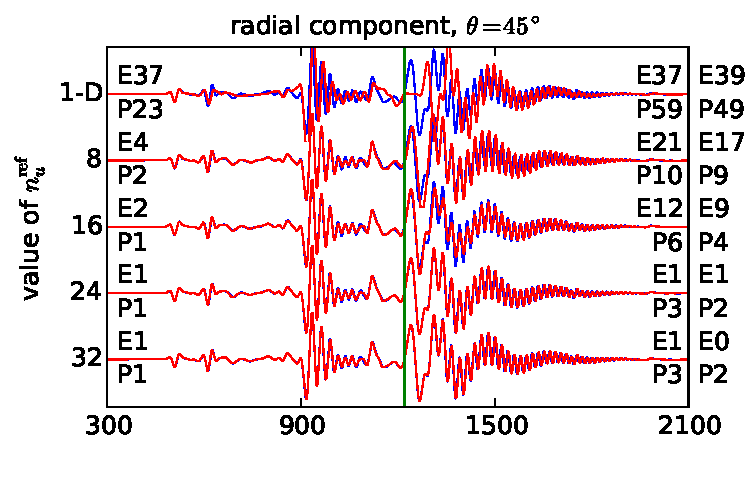
\includegraphics[width=.35\textwidth]{fig/conv_seism/VIR_s3_17_45xxx_R.pdf}\hspace{-15pt}
  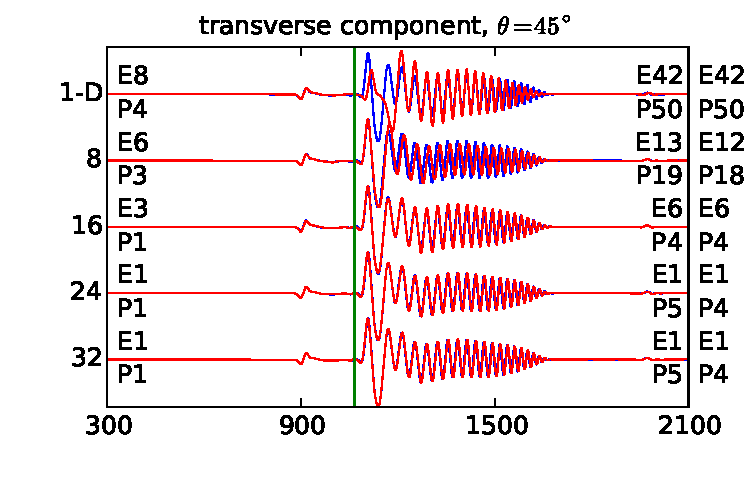
\includegraphics[width=.35\textwidth]{fig/conv_seism/VIR_s3_17_45xxx_T.pdf}\hspace{-15pt}
  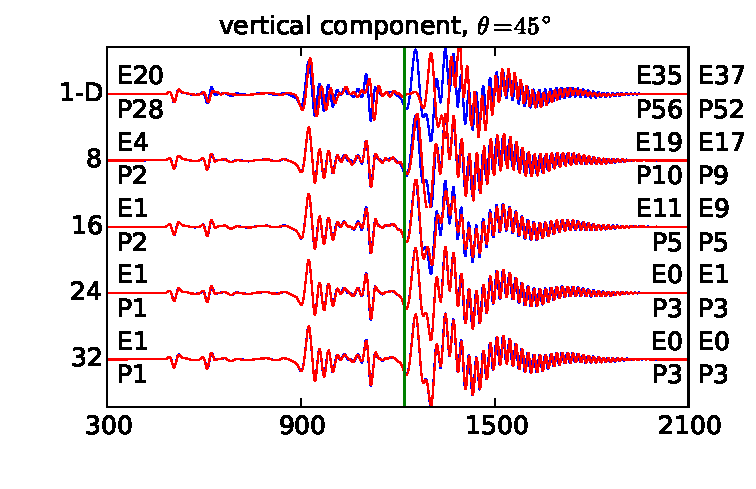
\includegraphics[width=.35\textwidth]{fig/conv_seism/VIR_s3_17_45xxx_Z.pdf}\vspace{-10pt}
  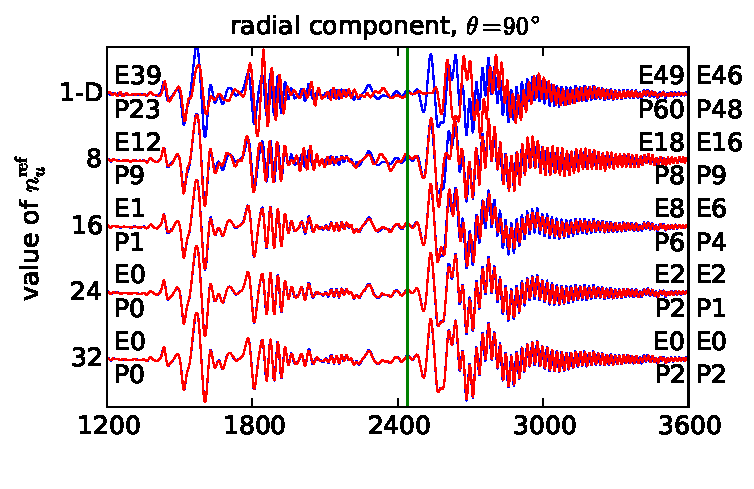
\includegraphics[width=.35\textwidth]{fig/conv_seism/VIR_s3_17_90xxx_R.pdf}\hspace{-15pt}
  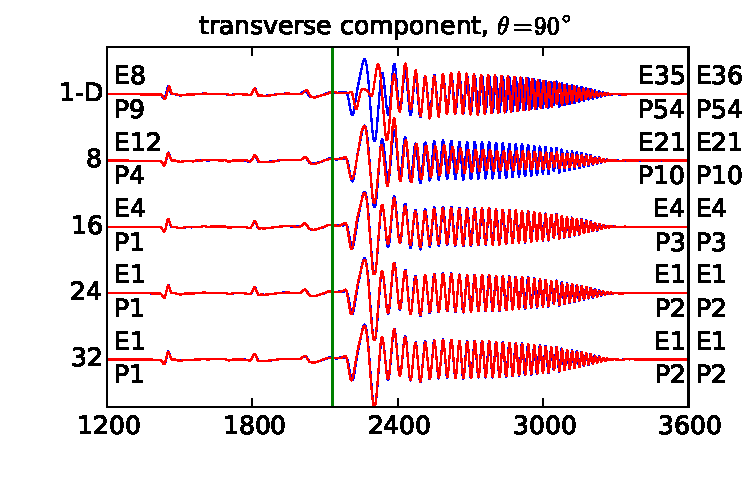
\includegraphics[width=.35\textwidth]{fig/conv_seism/VIR_s3_17_90xxx_T.pdf}\hspace{-15pt}
  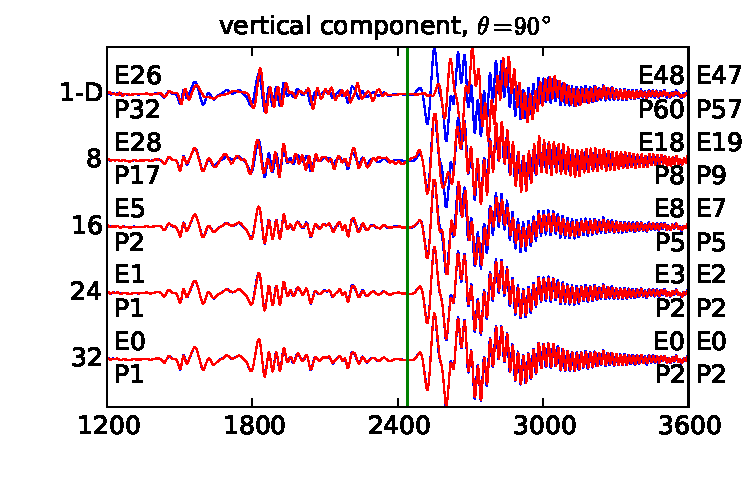
\includegraphics[width=.35\textwidth]{fig/conv_seism/VIR_s3_17_90xxx_Z.pdf}\vspace{-10pt}
  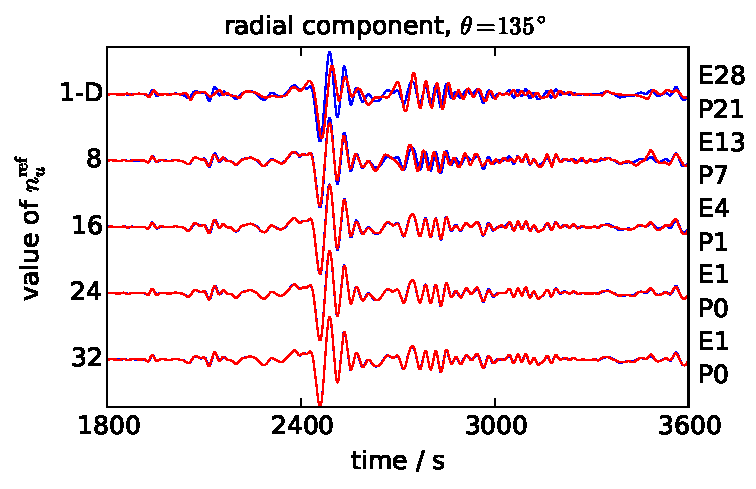
\includegraphics[width=.35\textwidth]{fig/conv_seism/VIR_s3_17_135xxx_R.pdf}\hspace{-15pt}
  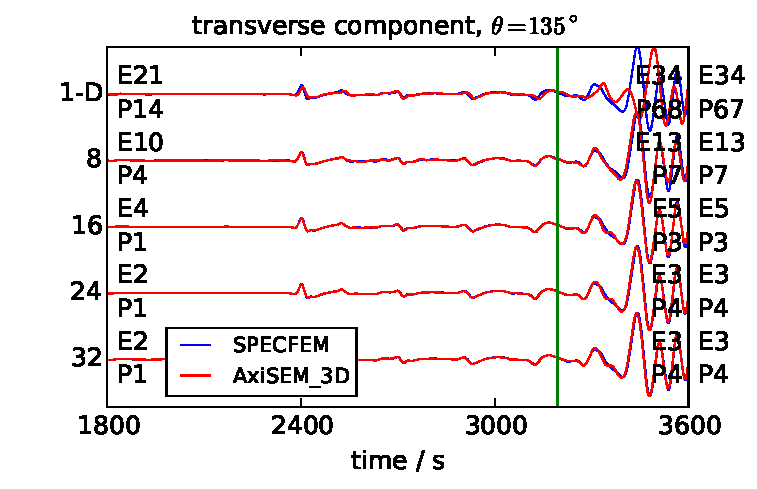
\includegraphics[width=.35\textwidth]{fig/conv_seism/VIR_s3_17_135xxx_T.pdf}\hspace{-15pt}
  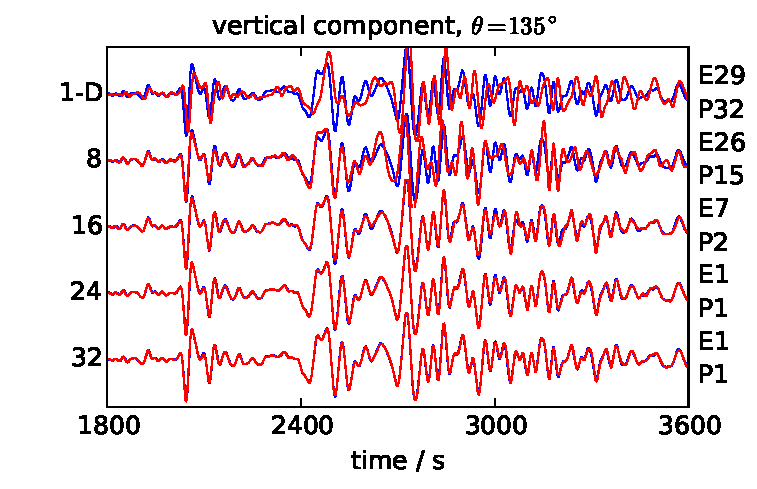
\includegraphics[width=.35\textwidth]{fig/conv_seism/VIR_s3_17_135xxx_Z.pdf}\vspace{-5pt}
  \caption{Comparisons of synthetic seismograms computed by SPECFEM and AxiSEM\_3D,
  as an illustration of convergence behavior of the Fourier spectral solution. 
  Simulation parameters: model = s362ani, $T_0\approx17\text{s}$, 
  source = VIR (12km, 37.91\degr N, 77.93\degr W, Virginia).
  The three receivers (red dots in Fig.~\ref{fig:rec})
  are all located on the meridian $\phi=180\degr$. 
  The first waveform pair in each figure is special, where we use 3-D model (s362ani)
  in SPECFEM but 1-D reference model (PREM) in AxiSEM\_3D, which gives
  an upper bound of misfits. The subsequent pairs are all 3-D model based, 
  following an integer (8, 16, 24 or 32) specifying $n_u^\text{ref}$ in \eqref{eq:nu}. 
  The symbols ``E$x$'' and ``P$y$'' should be interpreted as 
  $\mathtt{EM}=x\%$ and $\mathtt{PM}=y\%$, respectively.
  For each pair, such symbols from left to right indicate the TF-misfits 
  over the three windows $[0,t_\text{surf}]$, $[t_\text{surf},t_\text{max}]$ 
  and $[0,t_\text{max}]$, respectively,
  where $t_\text{max}=1\text{h}$ and
  $t_\text{surf}$ an approximate arrival time for surface waves 
  (green vertical line). Note that we only show the 
  full-length window misfits for the radial and vertical components
  at $\theta=135\degr$ because the Reighley wave has not arrived 
  ($t_\text{surf}>t_\text{max}$).
  Low frequency components below 0.005Hz are filtered.}
  \label{fig:empml}
\end{figure*}

\begin{figure}
  \centering
  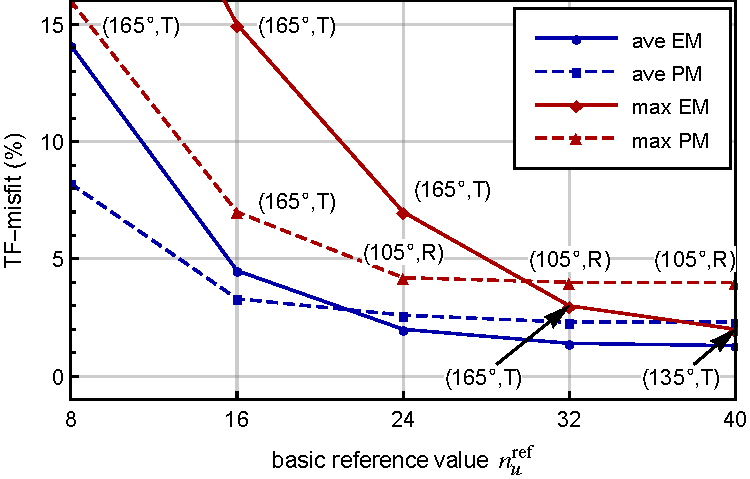
\includegraphics[width=.46\textwidth]{fig/conv_empm/nu_misfit.pdf}
  \caption{Convergence of global average and maximum TF-misfits. 
  Simulation parameters: model = s362ani, $T_0\approx17\text{s}$, 
  source = VIR (12km, 37.91\degr N, 77.93\degr W, Virginia).
  The plotted misfits are computed on the full-length window with 
  $t_\text{max}=1\text{h}$ and modified by 1-D results.
  The parentheses near a data point show the distance and 
  direction (R = radial, T = transverse, Z = vertical) 
  of the maximum misfit.} 
  \label{fig:empm}
\end{figure}

%~~~~~~~~~~~~~~~~~~~~~~~~~~~~~~~~~~~~~~~~~~~~~~~~~~~~~
\subsection{Frequency-dependence of $n_u$}
\label{sec:benfreq}
In Section~\ref{sec:strong}, we have shown that the cost of the method
scales with $n_u\omega^3$ for a specific model, compared to that of 3-D 
methods that scales with $\omega^4$.
Hence, the relation between $n_u$ and $\omega$ dominates the 
relative efficiency. 
Unfortunately, such a relation has not been theoretically established. 
Here we investigate it numerically. 
For this purpose, we fix the order parameter $n_u^\text{ref}$ at 24, but 
change the dominant period $T_0$ from 34s down to 11s, based on the same 
forward problem used in the previous subsection. 

As shown in Table~\ref{tab:freq}, the average misfits remain at the same 
level (sometimes even decrease) as $T_0$ falls off, 
suggesting that $n_u$ might be independent of
$\omega$, or, to say the least, should have a weak $\omega$-dependence. 
Such a numerical observation greatly benefits high frequency applications
owing to an implied scaling factor of $\omega^3$. 
We shall verify this observation with other Earth models 
in Section~\ref{sec:perf}. 

To visualize the goodness-of-fit, we display waveform comparisons
at $T_0\approx11\text{s}$ in Fig.~\ref{fig:freq} and Fig.~\ref{fig:freq2}. 
The former shows the vertical component on the meridional section $\phi=180\degr$
(green arc in Fig.~\ref{fig:rec}),
where a few phases of interests are magnified; 
and the latter shows the transverse component on the two 
circles of latitude at $\theta=60\degr$ and $\theta=120\degr$
(blue rings in Fig.~\ref{fig:rec}), respectively. 
Note that though we only compare waveforms on the surface,
the good fit of body wave phases, both direct and multiple, should imply 
a good fit of the interior wavefield. 

\begin{table}
\begin{minipage}{\columnwidth}
\caption{Average TF-misfits ($\%$) at different dominant periods.}
\label{tab:freq}
\setlength{\tabcolsep}{.28cm}
\begin{tabular*}{\textwidth}{cccccccc}
$T_0$ / s & $\mathtt{NEX}$ & $\mathtt{EM_B}$ & $\mathtt{PM_B}$ & 
$\mathtt{EM_S}$ & $\mathtt{PM_S}$ & $\mathtt{EM}$ & $\mathtt{PM}$\\[2pt]
\hline
34 & 128 &
1 {\scriptsize(T)}&
0 {\scriptsize(T)}&
1 {\scriptsize(T)}&
1 {\scriptsize(T)}&
1 {\scriptsize(T)}&
1 {\scriptsize(T)}\\[2pt]
23 & 192 &
1 {\scriptsize(T)}&
1 {\scriptsize(T)}&
1 {\scriptsize(T)}&
2 {\scriptsize(T)}&
2 {\scriptsize(T)}&
2 {\scriptsize(T)}\\[2pt]
17 & 256 &
2 {\scriptsize(T)}&
1 {\scriptsize(T)}&
2 {\scriptsize(R)}&
3 {\scriptsize(T)}&
2 {\scriptsize(T)}&
3 {\scriptsize(T)}\\[2pt]
14 & 320 &
2 {\scriptsize(T)}&
1 {\scriptsize(T)}&
2 {\scriptsize(R)}&
3 {\scriptsize(T)}&
2 {\scriptsize(T)}&
3 {\scriptsize(T)}\\[2pt]
11 & 384 & 
2 {\scriptsize(T)}&
1 {\scriptsize(T)}&
1 {\scriptsize(R)}&
2 {\scriptsize(T)}&
2 {\scriptsize(T)}&
2 {\scriptsize(T)}\\[2pt]
\hline
\end{tabular*}
\\\\
Simulation parameters: model = s362ani, $n_u^\text{ref}=24$, 
source = VIR (12km, 37.91\degr N, 77.93\degr W, Virginia).
The subscripts $\mathtt{B}$ and $\mathtt{S}$ specify the windows 
governed by body and surface waves, respectively.
The parentheses indicate the displacement component 
(R = radial, T = transverse, Z = vertical) of the leading misfit, 
the maximum among the three directions.
\end{minipage}
\end{table}

\begin{figure*}
  \centering
  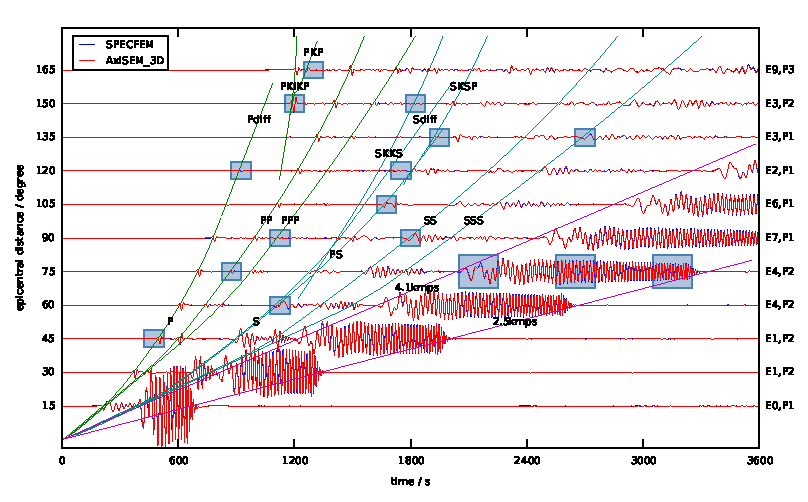
\includegraphics[width=\textwidth]{fig/section/VIR_s3_11_24.pdf}\vspace{-10pt}
  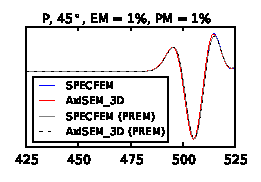
\includegraphics[width=.25\textwidth]{fig/section/1.pdf}\hspace{-5pt}
  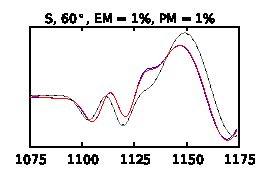
\includegraphics[width=.25\textwidth]{fig/section/2.pdf}\hspace{-5pt}
  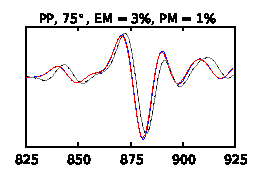
\includegraphics[width=.25\textwidth]{fig/section/3.pdf}\hspace{-5pt}
  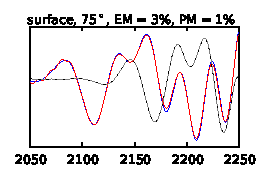
\includegraphics[width=.25\textwidth]{fig/section/4.pdf}\vspace{-5pt}
  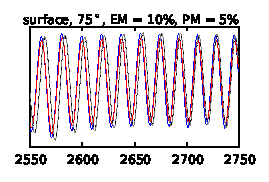
\includegraphics[width=.25\textwidth]{fig/section/5.pdf}\hspace{-5pt}
  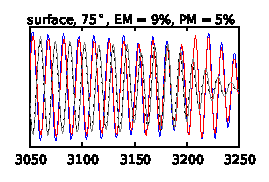
\includegraphics[width=.25\textwidth]{fig/section/6.pdf}\hspace{-5pt}
  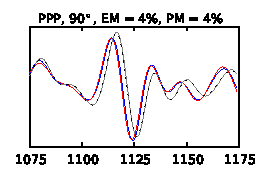
\includegraphics[width=.25\textwidth]{fig/section/7.pdf}\hspace{-5pt}
  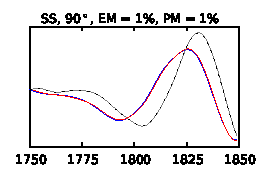
\includegraphics[width=.25\textwidth]{fig/section/8.pdf}\vspace{-5pt}
  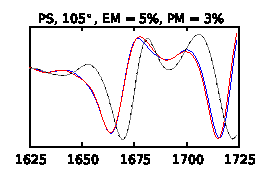
\includegraphics[width=.25\textwidth]{fig/section/9.pdf}\hspace{-5pt}
  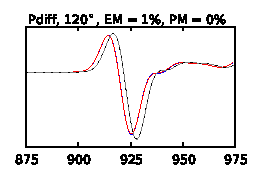
\includegraphics[width=.25\textwidth]{fig/section/10.pdf}\hspace{-5pt}
  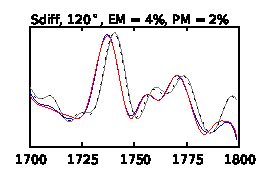
\includegraphics[width=.25\textwidth]{fig/section/11.pdf}\hspace{-5pt}
  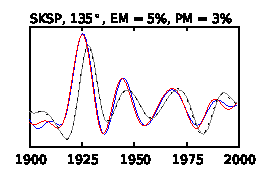
\includegraphics[width=.25\textwidth]{fig/section/12.pdf}\vspace{-5pt}
  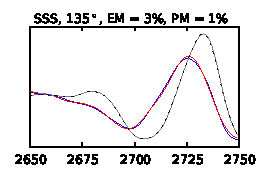
\includegraphics[width=.25\textwidth]{fig/section/13.pdf}\hspace{-5pt}
  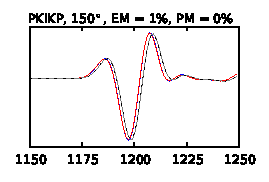
\includegraphics[width=.25\textwidth]{fig/section/14.pdf}\hspace{-5pt}
  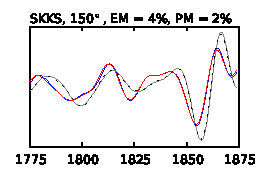
\includegraphics[width=.25\textwidth]{fig/section/15.pdf}\hspace{-5pt}
  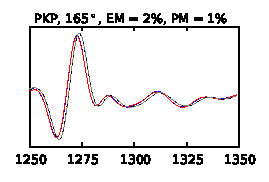
\includegraphics[width=.25\textwidth]{fig/section/16.pdf}\vspace{-5pt}
  \caption{Comparisons of synthetic seismograms (vertical component) computed 
  by SPECFEM and AxiSEM\_3D, with a few significant seismic phases magnified.
  Simulation parameters: model = s362ani, 
  $T_0\approx11\text{s}$, $n_u^\text{ref}=24$, 
  source = VIR (12km, 37.91\degr N, 77.93\degr W, Virginia). 
  The receivers are all located on the meridian $\phi=180\degr$ (
  green arc in Fig.~\ref{fig:rec}). 
  The amplitudes have been scaled with a factor of $\sqrt\theta$ 
  to identify most phases at all distances. 
  Low frequency components below 0.005Hz are filtered.
  The symbols after each waveform pair indicate the TF-misfits over the full-length 
  window, e.g., ``E5, P2'' means $\mathtt{EM}=5\%$ and $\mathtt{PM}=2\%$.
  We additionally plot the synthetics for the 1-D reference model PREM in the 
  magnified windows to emphasize the lateral scattering effects
  and, incidentally, to exhibit ``perfect'' benchmark for 1-D models. 
  The travel time curves are computed based on 1-D reference model ak135 
  \cite[]{kennett1995constraints} using OBSPY.TAUP \cite[]{krischer2015obspy}. }
  \label{fig:freq}
\end{figure*} 

\begin{figure}
  \centering
  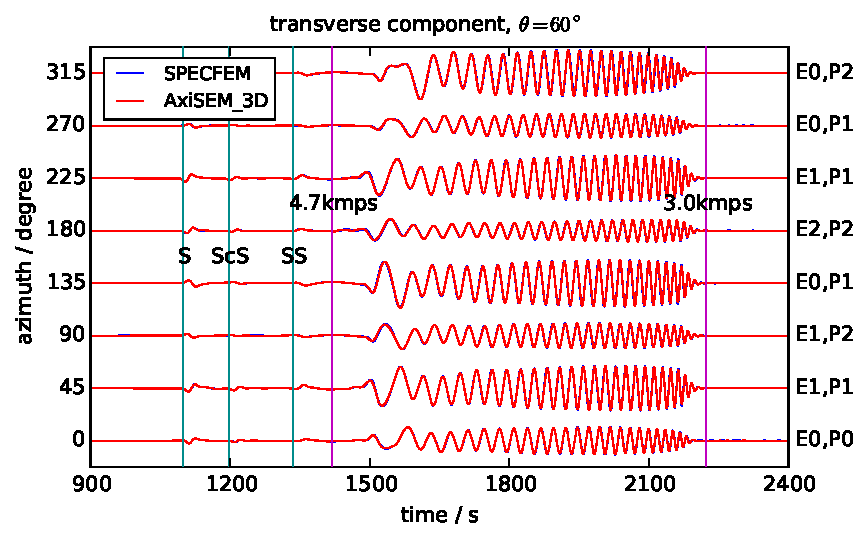
\includegraphics[width=.47\textwidth]{fig/ring/VIR_s3_11_60.pdf}\\\vspace{-5pt}
  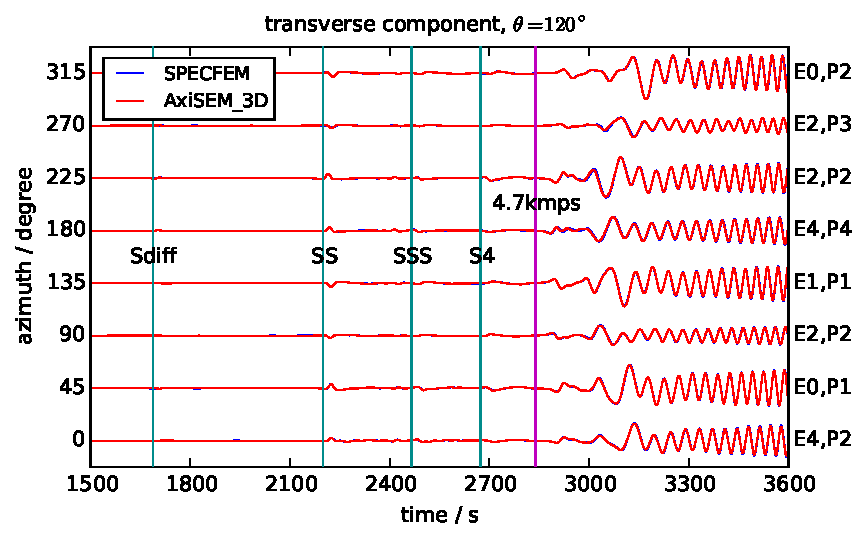
\includegraphics[width=.47\textwidth]{fig/ring/VIR_s3_11_120.pdf}\vspace{-5pt}
  \caption{Comparisons of synthetic seismograms (transverse component) computed 
  by SPECFEM and AxiSEM\_3D. The receivers are located on the two circles of latitude 
  at $\theta=60\degr$ and $\theta=120\degr$ (blue rings in Fig.~\ref{fig:rec}), 
  respectively. Other figure settings are identical to Fig.~\ref{fig:freq}.}
  \label{fig:freq2}
\end{figure}

%~~~~~~~~~~~~~~~~~~~~~~~~~~~~~~~~~~~~~~~~~~~~~~~~~~~~~
\subsection{Source influence}
\label{sec:bensrc}
Because our method necessitates a source-centered coordinate 
system, we also need to verify the source dependence of accuracy. 
We select eight earthquakes located worldwide, including four shallow, 
two intermediate and two deep earthquakes, as shown in Fig.~\ref{fig:cmt}.
The period is fixed at 17s. The results summarized in Table~\ref{tab:cmt}
indicate that source location and depth scarcely affect the goodness-of-fit,
which, in turn, suggests a robustness of the method to the locality 
of structural complexity.

\begin{figure}
  \centering
  \includegraphics[width=.48\textwidth]{fig/cmt/cmt.pdf}
  \caption{Map of earthquake sources. The shallow, intermediate 
  and deep sources are colored respectively blue, green and red,
  with beachball radii scaled by magnitude. }
  \label{fig:cmt}
\end{figure}   

\begin{table}
\begin{minipage}{\columnwidth}
\caption{Average TF-misfits ($\%$) for different earthquake sources.}
\label{tab:cmt}
\setlength{\tabcolsep}{.255cm}
\begin{tabular*}{\textwidth}{cccccccc}
Label & $d$ / km & $\mathtt{EM_B}$ & $\mathtt{PM_B}$ & 
$\mathtt{EM_S}$ & $\mathtt{PM_S}$ & $\mathtt{EM}$ & $\mathtt{PM}$\\[2pt]
\hline
VIR & \ \ 12.00 &
3 {\scriptsize(T)} &
1 {\scriptsize(T)} &
2 {\scriptsize(R)} &
3 {\scriptsize(T)} &
2 {\scriptsize(T)} &
3 {\scriptsize(T)} \\[2pt]
ITA & \ \ 15.00 &
1 {\scriptsize(T)} &
0 {\scriptsize(T)} &
2 {\scriptsize(R)} &
1 {\scriptsize(T)} &
2 {\scriptsize(T)} &
1 {\scriptsize(T)} \\[2pt]
PAK & \ \ 15.38 &
1 {\scriptsize(T)} &
0 {\scriptsize(T)} &
3 {\scriptsize(T)} &
3 {\scriptsize(T)} &
2 {\scriptsize(T)} &
3 {\scriptsize(T)} \\[2pt]
ATL & \ \ 21.81 &
1 {\scriptsize(T)} &
0 {\scriptsize(T)} &
2 {\scriptsize(R)} &
2 {\scriptsize(T)} &
1 {\scriptsize(T)} &
2 {\scriptsize(T)} \\[2pt]
ALS & 129.76 &
1 {\scriptsize(T)} &
0 {\scriptsize(Z)} &
1 {\scriptsize(R)} &
1 {\scriptsize(T)} &
1 {\scriptsize(T)} &
1 {\scriptsize(Z)} \\[2pt]
NZL & 165.12 &
1 {\scriptsize(T)} &
0 {\scriptsize(T)} &
2 {\scriptsize(T)} &
0 {\scriptsize(T)} &
2 {\scriptsize(T)} &
0 {\scriptsize(T)} \\[2pt]
BOL & 647.10 &
2 {\scriptsize(T)} &
1 {\scriptsize(Z)} &
3 {\scriptsize(T)} &
1 {\scriptsize(T)} &
2 {\scriptsize(T)} &
1 {\scriptsize(Z)} \\[2pt]
JPN & 680.70 &
1 {\scriptsize(T)} &
0 {\scriptsize(T)} &
2 {\scriptsize(R)} &
1 {\scriptsize(R)} &
1 {\scriptsize(T)} &
1 {\scriptsize(T)} \\[2pt]
\hline
\end{tabular*}
\\\\
Simulation parameters: model = s362ani, $T_0\approx17\text{s}$, 
$n_u^\text{ref}=24$. Other table settings are identical to 
Table~\ref{tab:freq}.
\end{minipage}
\end{table}

\section{Performance}
\label{sec:perf}
Let us first sum up our existing knowledge of the cost characteristics of 
the method. Section~\ref{sec:strong} first suggests a cost of 
$O\left(n_c n_u \omega^3\right)$, where $n_c$ and $n_u$ respectively reflect the 
azimuthal complexity of the model and the wavefield.
The factor $n_c n_u$ accounts for the $\phi$-dimension, 
and $\omega^3$ for the 2-D meridian domain $\left(s,z\right)$ 
plus one time dimension $t$. 
In Section~\ref{sec:benfreq}, we have numerically observed that $n_u$ tends to
be frequency independent. 
Therefore, for a specific model ($n_c=\text{const}$), 
the cost of the method should scale with $\omega^3$. 
Since the cost of a 3-D method scales with $\omega^4$
(3 spatial dimensions plus one time dimension), it can be predicted that 
our method should become increasingly faster than 
3-D methods as the frequency increases.

In this section, we compare the performance of SPECFEM and AxiSEM\_3D
using three global tomographic models, s362ani, s20rts and s40rts, 
with the dominant period ranged from 34s to 11s. We follow the same 
accuracy criteria defined in the benchmark section and consider 
all the earthquake sources in Fig.~\ref{fig:cmt}.
 
Repeating the convergence test in Section~\ref{sec:benconv},
we find that the accuracy criteria can be satisfied when 
$n_u^\text{ref}$ reaches 24 for s20rts and 32 for s40rts.
The $n_u^\text{ref}$ values obtained at $T_0\approx17\text{s}$ turn out to be 
sufficient at $T_0\approx11\text{s}$ as well, reconfirming the 
frequency-independence of $n_u$.
Recalling Fig.~\ref{fig:spectra},
the maximum values of $n_c$ for the three models are respectively 
22 (s362ani), 20 (s20rts) and 40 (s40rts), while
the least $n_u^\text{ref}$'s turn out to be 24, 24 and 32 respectively,
so we can assert that $n_u$ should increase with $n_c$. 
This is actually all too obvious
because the complexity of the wavefield should certainly
grow with that of the model.
Nevertheless, only three models are far from enough to establish 
a solid relation between $n_u$ and $n_c$.
Eventually, we may rewrite the cost of the method as 
$O\left(n_c^q \omega^3\right)$, where $q$ is a positive real constant and $q>1$. 
In other words, the cost strongly depends on the lateral complexity 
of the model, inasmuch as $n_c$ controls both the size ($n_u$) and the 
bandwidth of the dimension-reduced system \eqref{eq:band2d}. 

The actual computational costs summarized in Table~\ref{tab:perf}
well support our above speculations:
\begin{itemize}
\item AxiSEM\_3D prevails over SPECFEM for the three tomographic models 
across the considered frequency band;
\item the maximum speedup reaches 85 for s20rts at 11s;
\item the speedup steadily increases with frequency;  
\item the costs for s20rts and s362ani are similar while that for s40rts 
nearly doubles.
\end{itemize}
It is also observed that the cost of AxiSEM\_3D may be further reduced by 
approximately 30\% for deep earthquakes, 
such as BOL and JPN in Fig.~\ref{fig:cmt}, 
as we may switch off the resolution enhancement for surface waves 
by fixing $F_d=1$ in \eqref{eq:nu}.

Fig.~\ref{fig:logcost} shows an order-of-magnitude cost measurement, 
based on real simulations. 
As emphasized by the dashed vertical lines,
the advantage of AxiSEM\_3D grows with frequency. 
In light of this trend, we might achieve real-time simulations at 5s
only with a few hundred cores. We will verify such 
attractive extrapolation in the near future.
The low-frequency trend, however, predicts a critical period above which 
SPECFEM should excel (a result of the constant prefactor $n_c^q$), 
which, however, remain undiscovered due to the mesh restriction
of SPECFEM ($T_0 \le 68\text{s}$ or $\mathtt{NEX} \ge 64$).

\begin{table}
\begin{minipage}{\columnwidth}
\caption{Computational costs of SPECFEM and AxiSEM\_3D for 
1h-length synthetics.}
\label{tab:perf}
\setlength{\tabcolsep}{.3cm}
\begin{tabular*}{\textwidth}
  {lllll}
$T_0/\text{s}$ & \enspace SPEC & Axi (s20rts) & Axi (s362ani) & Axi (s40rts)\\[2pt]
\hline
 \ \ 34 & \enspace\enspace73.6   & 
 \ \enspace2.1 \ \ (34) & 
 \ \ \enspace2.3 \ \ (32) & 
 \ \enspace4.2 \ \ (17) \\[2pt]
 \ \ 23 & \enspace188.8  & 
 \ \enspace4.1 \ \ (47) & 
 \ \ \enspace4.3 \ \ (44) & 
 \ \enspace7.9 \ \ (24) \\[2pt]
 \ \ 17 & \enspace324.8  & 
 \ \enspace6.8 \ \ (48) & 
 \ \ \enspace7.2 \ \ (45) &        
  \       11.9 \ \ (27) \\[2pt]
 \ \ 14 & \enspace768.0  &        
 \ 12.6 \ \ (61) &        
 \ \ 13.3 \ \ (58) &        
 \ 22.3 \ \ (34) \\[2pt]
 \ \ 11 & 2046.7 &        
 \ 24.2 \ \ (85) &        
 \ \ 25.6 \ \ (80) &        
 \ 42.9 \ \ (48) \\[2pt]
\hline
\end{tabular*}
\\\\
The second column shows the SPECFEM CPU-hours for s362ani, those
for s20rts and s40rts being very similar.
The following three columns show the AxiSEM\_3D CPU-hours and the  
speedup rates (parenthesized) relative to SPECFEM. 
The CPU-hours are obtained on ARCHER, the latest UK national supercomputing 
service (\url{archer.ac.uk}). The system default (suggested) compiler 
options are applied for both codes, with enforced 
cache-optimized loop vectorization \cite[Chap 8,][]{deville2002high}.
For SPECFEM, all possible core numbers are tested for best performance,
while the AxiSEM\_3D results are obtained from serial simulations. 
\end{minipage}
\end{table}

\begin{figure}
  \centering
  \hspace{-10pt}\includegraphics[width=.495\textwidth]{fig/cost/cost.pdf} 
  \vspace{-20pt}
  \caption{Computational cost of global wavefield simulations in “real time” 
  (i.e., seismogram length equals wallclock simulation time) for different 
  methods. Each data point is based on actual runtime on ARCHER,
  and gives as a result the number of processors needed to achieve this, 
  assuming perfect scalability. The core numbers can also be interpreted 
  as the CPU-hours required to produce 1~h length synthetics.}
  \label{fig:logcost}
\end{figure} 


\section{Discussion}
The nature of seismic point sources and realistic Earth models 
bestows azimuthal smoothness on global seismic wavefields (e.g. Fig.~\ref{fig:snapshot}). 
To honor and exploit this property, we parameterize 3-D wavefields
in terms of Fourier series over the azimuthal dimension while
retaining a spectral-element discretization in the 2-D meridian domain,
such that the number of unknowns and thus the computational cost 
can be remarkably reduced compared to full 3-D discretization.

We reduce the 3-D equations of motion to 
an algebraic system of coupled 2-D meridian equations,
and implement a 2-D SEM, AxiSEM\_3D, to solve the dimension-reduced system.
Numerical benchmarks show excellent agreement 
between AxiSEM\_3D and SPECFEM3D\_GLOBE 
\cite[]{komatitsch2002spectralI,komatitsch2002spectralII},
an independent full 3-D SEM, 
for state-of-the-art global tomographic models
across a frequency range typically employed in global waveform modeling 
and tomography, considering material anisotropy, attenuation and the fluid outer core. 
To the best of our knowledge, this is the first benchmark
between two independent methods for global wave propagation in 3-D Earth models. 

Upon satisfying specific full-waveform-based accuracy criteria, 
performance comparisons manifest large computational advantage of our method.
As shown in Fig.~\ref{fig:logcost}, AxiSEM\_3D is strikingly faster than SPECFEM
for the considered tomographic models across the period range [34s, 11s], 
attaining a maximum speedup of 85 for s20rts at 11s. 
Most importantly, Fig.~\ref{fig:logcost} reveals the trend that such 
computational advantage steadily grows with frequency, 
as predicted by the $O(\omega^3)$ cost
for AxiSEM\_3D, in contrast to $O(\omega^4)$ for 3-D methods such as SPECFEM.
The $\omega^3$ scalability will greatly benefit high-frequency applications,
e.g., $\sim$5s in the near future. 
The large performance boost of wavefield simulations will inevitably 
encourage both data utilization and methodological advances in tomography.  

\subsection{Model-adaptive cost}
\label{sec:adapt}
The model-dependent cost characteristic distinguishes our method from 
full 3-D methods. As shown in Fig.~\ref{fig:logcost}, our method 
bridges the gap between fast axisymmetric methods (AxiSEM) and 
slower but comprehensive 3-D methods (SPECFEM), based on a sort of 
``intelligent recognition'' of model complexity. Such model adaptivity
is particularly favorable for global seismology where 
the Earth models, both for forward modeling and tomographic purposes,  
tend to be smooth with respect to seismic wavelengths. 
We defer an in-depth analysis of the method's performance with respect to 
the ratio of heterogeneity and wavelength and other relevant 
parameters to a future study.

The convergence of the method enables a controllable 
trade-off between accuracy and performance by prescribing the lateral
resolution of solution ($n_u$), e.g., 
the empirical equation \eqref{eq:nu} aimed at a uniform
accuracy throughout space (see e.g. Fig.~\ref{fig:freq} and Fig.~\ref{fig:freq2}), 
in conjunction with the choice of $n_u^\text{ref}$  
that controls the global accuracy.
This can be even more attractive in a local sense 
(as $n_u$ can be assigned pointwise), i.e., enhancing local complexities   
(e.g. surface waves in the crust) will not drastically affect overall 
performance.

For tomographic purposes, such flexibility extends one step further from solution 
space (by prescribing $n_u$) to model space (by prescribing $n_c$), allowing 
for the construction of ``hypothetical'' but 
most relevant and efficient 3-D background models.
Should one wish to focus on resolving 
a given target region on account of specific seismic phases, 
one may for instance reduce the cost by assuming spherical symmetry of 
the less relevant regions, thereby enjoying a bulk cost closer to the 1-D 
AxiSEM method without depreciating the results.
For instance, \cite{hosseini2015multifrequency} use diffracted body waves 
in the deep mantle; in this case, we may start from a 3-D background model 
that permits well-accepted, long-wavelength 3-D structures in the lower 
mantle, such that the excluded shallower features do not distort the 
used phases to a notable extend.

\subsection{Aspherical geometry}
\label{sec:geo}
Currently, our method requires the Earth model to be an exact 
spheroid to preserve axisymmetric geometry after source polarization. 
Such a restriction should be imposed not only on the outer surface, 
but also on all internal solid-solid and solid-fluid boundaries, 
preventing the introduction of Earth's ellipticity as well as topography 
on the surface and the internal discontinuities such as Moho and 
the core-mantle boundary.
The absent topography on the surface and Moho limits our method such that 
crustal models can be incorporated only via 3-D volumetric perturbations. 

A newly suggested remedy based on ``particle relabeling'' 
\cite[]{attar2016particle} emerges as a solution to this limitation.
In the theory of \cite{attar2016particle}, geometric perturbations can be mapped exactly into 
volumetric heterogeneity while preserving the form of the equations of motion. 
For ellipticity, the geometric perturbation is small and smooth, 
so the induced volumetric perturbations on physical properties will be
limited to a very few lower orders (very small $n_c$), and thus has less
performance influence. For 3-D crusts, however, the localized
lateral gradients on the surface and Moho may introduce higher complexity
to the physical space, increasing the computational cost to some extent. 
Nevertheless, we expect our method to maintain its advantage based on two reasons. 
First, recent global crustal models do not require very large $n_c$ to describe 
the lateral variations of material properties,
e.g., $n_c\le90$ for Crust2.0 \cite[]{bassin2000current} and
$n_c\le180$ for Crust1.0 \cite[]{laske2013update}. 
Furthermore, since 3-D crustal structures mainly impact surface waves, 
we possibly only have to strengthen the surface resolution by increasing $F_d$ 
in \eqref{eq:nu}, with a small fraction of elements affected.

% 
% \textit{Ellipticity and topography}.
% Because such geometric restrictions
% may produce visible and recordable errors when comparing to observed
% data, corrections may be imperative for specific cases of seismic data analysis. 
% In addition to conventional corrections \cite[Chap
% 13,][]{nolet2008breviary}, one may consider homogenization techniques
% for internal boundary topography, or off-loading the topography to
% intra-element polynomial expansions. Furthermore,
% a recently proposed method based on particle relabeling  
% \cite[]{attar3001particle} looks promising as an ultimate solution to this restriction.
% 
% \textit{Earth rotation}.
% Unless polar sources are of interest, 
% the method in its current incarnation cannot accommodate the effect 
% of Earth rotation due to the axial symmetry of the source. However, rotational effects come into 
% play only at long periods ($\>100s$) which are not seen as the
% ultimate target parameter space of our method which performs better
% at higher frequencies.
% 
% \textit{3-D crusts and internal topography}.
% Three-dimensional crustal structures are currently not implemented,
% but this shall be added and tested in future work.
% 3-D crustal models will certainly affect the 
% computational cost to some extent, but the favorable efficiency of the method
% is expected to remain for two reasons. First, recent global crust models do not require very 
% large $n_c$, e.g., $n_c\le90$ for Crust2.0 \cite[]{bassin2000current} and
% $n_c\le180$ for Crust1.0 \cite[]{laske2013update}, which, if seen as a
% multiplicative cost factor in Fig.~\ref{fig:logcost} seems to remain
% in a rather favourable realm. Furthermore, 
% since 3-D crustal structures mainly impact surface waves, we possibly 
% only have to strengthen the surface resolution by increasing $F_d$ 
% in \eqref{eq:nu}, with a tiny fraction of elements affected. 
% Our method allows topography on solid-solid discontinuities such as Moho
% and those in s362ani. We will examine how these internal interfaces can be approximated 
% by either a locally undulated 2-D mesh or by homogenization. 

\subsection{Adjoint tomography}
Our method is incapable of handling off-axis sources, which means
in the case of multiple simultaneous point sources, such as adjoint
simulations \cite[]{tromp2008spectral, liu2008finite} or simulations upon 
finite-fault sources, a number of individual runs must be carried out for 
each source location. 
Though principally doable, such a remedy hampers the computational superiority of the method. 
For adjoint tomography, however, this can be counterbalanced by the 
ability to perform Gauss-Newton iterations using the approximate Hessian 
\cite[Chap 10,][]{nocedal2006numerical} in addition to the gradient, 
leading to accelerated convergence and enabling new approaches to study the 
resolution of the resulted model. Furthermore, 
adjoint wavefields for fixed source locations may be re-used for different events 
in case the entire spatio-temporal wavefield solution can be stored (note that
our method is much more memory-efficient than 3-D methods
because of the azimuthal smoothness of wavefields). 

\subsection{Technical aspects}
Currently, the development of AxiSEM\_3D still remains in early
stages. Below we introduce two computational features to be addressed 
in the near future.

\textit{Parallelization}.
The implementation of AxiSEM\_3D is based on the existing 
package AxiSEM, whose scaling behavior has been verified for more than 
8000 cores on many HPC infrastructures \cite[]{nissen2014axisem}. 
The existent 2-D domain decomposer achieves exact load balancing 
by distributing an equal amount of elements to each
processor, as all elements are equally costly in AxiSEM.
However, in AxiSEM\_3D, elemental costs drastically vary 
owing to different local complexities (and thus different Fourier spectral orders) 
in both the model space 
(e.g. Fig.~\ref{fig:spectra}) and the solution space (e.g. Fig.~\ref{fig:nu}).
We thus require a more general decomposer capable of load weighting.
Currently, a new decomposer relying on the mature package 
METIS \cite[]{lasalle2015efficient} is being tested. 
Complete load-balancing is theoretically achievable because 
the elemental costs are predefined.
As roughly estimated from Fig.~\ref{fig:logcost},
we expect to approach a realtime simulation 
(seismogram length equals wallclock simulation time)
at a dominant period of 5s on a few hundred cores.

\textit{Adaptive optimization of $n_u$.}
Based on a large number of trial simulations, we developed
the empirical equation \eqref{eq:nu} to determine the 
Fourier spectral order $n_u\left(s,z\right)$, taking into account some 
first-order propagation characteristics.
Though the empirical equation \eqref{eq:nu} proves robust and efficient
for typical tomographic models, an optimal $n_u\left(s,z\right)$ may be further 
constructed via adaptive pre-simulations at lower frequencies, based on 
the observed frequency-independence of $n_u\left(s,z\right)$. 
First, we may generate a relatively sparse 2-D mesh and set the upper 
limit of $n_u$ to a large number at each GLL point. Then we 
propagate waves on the sparse mesh and at each time step filter out higher
order modes with small total energy. The obtained 
$n_u\left(s,z\right)$ can then be repeatedly used in higher frequency simulations. 
In doing so, we maximize the performance by uniforming the accuracy over
the entire domain. 
% Two major bottlenecks of our method exist:
% The incapability of handling off-axis sources
% (Section~\ref{sec:offaxis}), as well as a surging cost in the
% asymptotic case of small-scale structures and corresponding wavefield
% complexities that necessitate a higher Fourier expansion order. For
% the time being, however, we showed that our method performs well for
% all considered tomographic models. We will now briefly discuss future
% refinements to the method to estimate its adaptability to hypothetical
% models with small-scale structures as well as issues arising from the
% axial source. 



\bibliographystyle{gji}
\bibliography{axi3d}

\begin{acknowledgments}
We are grateful to Karin Sigloch, Kasra Hosseini and Simon St\"ahler 
for insightful discussions and computing assistance, and to 
Maria Tsekhmistrenko and Lion Krischer for helping with data processing.
KL gratefully acknowledge the financial support
provided by the State Key Laboratory of Hydroscience and Engineering,
Tsinghua University under Grant SKLHSE-2014-C-01 and 
the National Natural Science Foundation of China under Grant 51409225.
Computations have been undertaken on the UK National Supercomputing Service 
(ARCHER) under TNM's NERC/EPSRC ARCHER leadership grant,
whose fast and accurate technical support is highly appreciated. 
\end{acknowledgments}

\appendix
\section{Fluid core}
\label{sec:fluid}
The Earth model may contain a couple of solid-fluid boundaries, 
collectively denoted $\Sigma$, as shown in Fig.~\ref{fig:crd}. 
The method requires axisymmetry of $\Sigma$ such that it can 
be generated by rotating the meridian arc $S$ about the axis $A$. 

Following \cite{chaljub2004spectral, 
nissen2007axisem}, we shall adopt a potential formulation in the fluid 
domain $\Omega_{\text{f}}$. Let $\mathbf{u} = \nabla\chi/\rho$,
such that the equations of motion \eqref{eq:eom3d} in $\Omega_{\text{f}}$
can be recast as
\begin{equation}
  \frac{\ddot{\chi}}{\kappa} = \nabla\cdot\left(
  \frac{\nabla\chi}{\rho}\right), \ \text{in} \ \Omega_{\text{f}},
\end{equation}
subject to solid-fluid boundary conditions
\begin{equation}
  \hat{\mathbf{n}}\cdot\mathbf{u}=\frac{\chi_{,r}}{\rho}
  \quad \text{and} \quad 
  \hat{\mathbf{n}}\cdot\mathbf{C}:\left(\nabla\mathbf{u}\right)= 
  \ddot{\chi}\hat{\mathbf{n}}, \quad \text{on} \ \Sigma,
\end{equation}
where $\kappa$ denotes the bulk modulus of the fluid media. 
The completeness of the above potential representation is 
guaranteed by the absence of toroidal motion within an inviscid fluid core.
Accordingly, the 3-D weak form \eqref{eq:3dweak} can be generalized as
\begin{align}
&  \langle \rho\ddot{\mathbf{u}},\mathbf{w}\rangle_{\Omega_\text{s}}\!+\!
  a_{\Omega_\text{s}}\left(\mathbf{u},\mathbf{w}\right)\!+\!
  \langle \ddot{\chi}\hat{\mathbf{n}},\mathbf{w}\rangle_{\Sigma}
  \!=\!\langle \mathbf{f},\mathbf{w}\rangle_{\Omega_\text{s}}
  ,\ \forall\mathbf{w}\ \text{in}\ \Omega_\text{s},
  \label{eq:3dweaks}\\[.5em]
&  \langle \ddot{\chi}/\kappa,w \rangle_{\Omega_\text{f}}\!+\!
  b_{\Omega_\text{f}}\left(\chi,w\right)\!-\!
  \langle \mathbf{u}, w\hat{\mathbf{n}}\rangle_{\Sigma}
  \!=\!0,\ \forall w\ \text{in}\ \Omega_\text{f},
  \label{eq:3dweakf}
\end{align}
where the bilinear form in $\Omega_\text{f}$ is defined as
\begin{equation}
  b_{\Omega_\text{f}}\left(\chi,w\right) \coloneqq
  \int_{\Omega_\text{f}} \frac{1}{\rho}
  \left(\nabla\chi\right) \cdot \left(\nabla w\right) \text{d}^{3}\mathbf{r}.
\end{equation}
Solid-fluid coupling effects are embodied by the third terms
on the left-hand side of \eqref{eq:3dweaks} and \eqref{eq:3dweakf}.

Similar to \eqref{eq:u_four}, we characterize the fluid potential $\chi$
in terms of Fourier series, i.e.,
\begin{align}
  &\chi\left(s,\phi,z;t\right) \simeq \sum_{|\alpha|\le n_u} 
  \chi^\alpha\left(s,z;t\right)\Psi^\alpha\left(\phi\right),\\[.5em]
  &w\left(s,\phi,z\right) =\sum_{|\beta|\le n_u} 
  w^\beta\left(s,z\right)\Psi^\beta\left(\phi\right).
\end{align}
Following the same steps in Appendix~\ref{sec:dweak}, we may extend 
the reduced weak form \eqref{eq:2dweak} to solid-fluid media as
\begin{equation}
  \begin{alignedat}{1}
    &\sum_{|\alpha|\le n_u} \left[ 
    \left\langle \rho^{-\left(\alpha+\beta\right)}
    \ddot{\mathbf{u}}^\alpha,\mathbf{w}^\beta \right\rangle _{D_\text{s}}
    + a_{D_\text{s}}^{-\left(\alpha+\beta\right)}
    \left(\mathbf{u}^\alpha,\mathbf{w}^\beta\right)\right] \\
    &+\left\langle \ddot{\chi}^{-\beta}\hat{\mathbf{n}},
    \mathbf{w}^\beta \right\rangle _{S}
    =\left\langle \mathbf{f}^{-\beta},\mathbf{w}^\beta \right\rangle 
    _{D_\text{s}}, 
    {\scriptsize
    \begin{array}{l}
      \forall \mathbf{w}^\beta\ \text{in}\ D_\text{s} \\[.3em]
      \forall \beta\in \{-n_u,...,n_u\}
    \end{array}
    },
  \end{alignedat}
\end{equation}
\begin{equation}
  \begin{alignedat}{1}
    & \left\langle 
    \ddot{\chi}^{-\beta}\Big/\kappa^{0}, w^\beta
    \right\rangle _{D_\text{f}}
    + b^0_{D_\text{f}}
    \left(\chi^{-\beta},w^\beta\right) 
    -\left\langle \mathbf{u}^{-\beta}, w^\beta \hat{\mathbf{n}}
    \right\rangle _{S}
    \\&=0, \quad \forall w^\beta\ \text{in}\ D_\text{f},
    \quad \forall \beta\in \{-n_u,\dots,n_u\},
  \end{alignedat}
  \label{eq:2dweakf}
\end{equation}
where the bilinear form in $D_\text{f}$ is defined as
\begin{equation}
  b^0_{D_\text{f}}\left(\chi^{\alpha},w^\beta\right) \coloneqq
  \int_{D_\text{f}} \frac{1}{\rho^0}
  \left(\chi^{\alpha}_{,i} w^{\beta}_{,i} -
  \alpha\beta \chi^{\alpha} w^{\beta}\right) s\,\text{d}s\text{d}z.
\end{equation}
The reduced weak form \eqref{eq:2dweakf} implies no mode coupling 
in the fluid domain, thanks to the spherical symmetry of 
the outer core, i.e., 
$\kappa\left(s,\phi,z\right)=\kappa^0\left(s,z\right)$ and $\rho\left(s,\phi,z\right)=\rho^0\left(s,z\right)$.

\section{Derivation of Dimension-reduced weak form}
\label{sec:dweak}
In this appendix, we derive the dimemsion-reduced weak form 
\eqref{eq:2dweak} from the 3-D weak form \eqref{eq:3dweak}.
Substituted with the Fourier characterizations \eqref{eq:f_four} and 
\eqref{eq:w_four}, the source term in \eqref{eq:3dweak} can be reduced 
in the following steps:
\begin{equation}
  \begin{alignedat}{1}
    &\langle \mathbf{f},\mathbf{w}\rangle _{\Omega} =
    \int_{\Omega}\mathbf{f}\cdot\mathbf{w}\text{d}^{3}\mathbf{r} \\&=
    \int_{\Omega} \sum_{|\alpha|\le n_f} f_i^\alpha \Psi^\alpha
    \sum_{|\beta|\le n_u}  w_i^\beta \Psi^\beta s\,\text{d}s\text{d}\phi \text{d}z \\&=
    \sum_{|\alpha|\le n_f} \sum_{|\beta|\le n_u}  
    \int_{D} f_i^\alpha w_i^\beta s\,\text{d}s\text{d}z 
    \int_{-\pi}^{\pi} \Psi^\alpha \Psi^\beta \text{d}\phi\\&=
    2\pi \sum_{|\beta|\le n_u} \int_{D} f_i^{-\beta} w_i^\beta s\,\text{d}s\text{d}z \\&=
    2\pi \sum_{|\beta|\le n_u} \left\langle \mathbf{f}^{-\beta},
    \mathbf{w}^{\beta}\right\rangle_{D},
  \end{alignedat}
  \label{eq:a1}
\end{equation}
where the third row is based on the integral equality \eqref{eq:ieq}
and the fourth row the orthogonality condition \eqref{eq:orth}.
Likewise, the mass and stiffness terms are respectively reduced as
\begin{equation}
  \begin{alignedat}{1}
    &\langle \rho \ddot{\mathbf{u}},\mathbf{w}\rangle _{\Omega} =
    \int_{\Omega} \rho \ddot{\mathbf{u}} \cdot\mathbf{w}\text{d}^{3}\mathbf{r} \\&=
    \int_{\Omega} \sum_{|\gamma|\le n_\rho} \rho^\gamma \Psi^\gamma
    \sum_{|\alpha|\le n_u} \ddot{u}_i^\alpha \Psi^\alpha
    \sum_{|\beta|\le n_u}  w_i^\beta \Psi^\beta s\,\text{d}s\text{d}\phi \text{d}z \\&=
    \sum_{|\gamma|\le n_\rho} \sum_{|\alpha|\le n_u} \sum_{|\beta|\le n_u}  
    \int_{D} \rho^\gamma u_i^\alpha w_i^\beta s\,\text{d}s\text{d}z 
    \int_{-\pi}^{\pi} \Psi^\gamma \Psi^\alpha \Psi^\beta \text{d}\phi\\&=
    2\pi \sum_{|\alpha|\le n_u} \sum_{|\beta|\le n_u} 
    \int_{D} \rho^{-\left(\alpha+\beta\right)} u_i^{\alpha} w_i^\beta s\,\text{d}s\text{d}z \\&=
    2\pi \sum_{|\alpha|\le n_u} \sum_{|\beta|\le n_u} 
    \left\langle \rho^{-\left(\alpha+\beta\right)} \ddot{\mathbf{u}}^{\alpha},
    \mathbf{w}^{\beta}\right\rangle_{D},
  \end{alignedat}
  \label{eq:a2}
\end{equation}
and
\begin{equation}
  \begin{alignedat}{1}
    & a_{\Omega}\left(\mathbf{u},\mathbf{w}\right)  =
    \int_{\Omega} \left(\nabla\mathbf{u}\right) :\mathbf{C}: \left(\nabla\mathbf{w}\right)
    \text{d}^{3}\mathbf{r} \\&=
    \int_{\Omega} \sum_{|\gamma|\le n_c} C^\gamma_{ijkl} \Psi^\gamma
    \sum_{|\alpha|\le n_u} u_{i;j}^\alpha \Psi^\alpha
    \sum_{|\beta|\le n_u}  w_{k;l}^\beta \Psi^\beta s\,\text{d}s\text{d}\phi \text{d}z \\&=
    \sum_{|\gamma|\le n_c} \sum_{|\alpha|\le n_u} \sum_{|\beta|\le n_u}  
    \int_{D} C^\gamma_{ijkl} u_{i;j}^\alpha w_{k;l}^\beta s\,\text{d}s\text{d}z 
    \int_{-\pi}^{\pi} \Psi^\gamma \Psi^\alpha \Psi^\beta \text{d}\phi\\&=
    2\pi \sum_{|\alpha|\le n_u} \sum_{|\beta|\le n_u} 
    \int_{D} C^{-\left(\alpha+\beta\right)}_{ijkl} u_{i;j}^\alpha w_{k;l}^\beta s\,\text{d}s\text{d}z \\&=
    2\pi \sum_{|\alpha|\le n_u} \sum_{|\beta|\le n_u} 
    a_{D}^{-\left(\alpha+\beta\right)}\left(\mathbf{u}^\alpha,\mathbf{w}^{\beta}\right).
  \end{alignedat}
  \label{eq:a3}
\end{equation}
Due to the arbitrariness of $\mathbf{w}$, we may drop the mode summations 
over $\beta$ in \eqref{eq:a1}-\eqref{eq:a3} and finally obtain
the dimension-reduced weak form \eqref{eq:2dweak}.



\bsp % ``This paper has been produced using the Blackwell
     %   Publishing GJI \LaTeXe\ class file.''

\label{lastpage}


\end{document}
